%styles
%Da Latex für englischsprachige Texte ausgerichtet ist,
%wird als Dokumentenklasse das "`scrbook"' von Markus Kohm verwendet.
%Dieses ist für deutschsprachige Texte ausgelegt.
%BCOR12mm: 12mm Bindekorrektur (Verbreiterung des linken Randes)
%DIV11: entspricht in etwas der geforderten Textgröße und Seitenränder
%titlepage: eine Titelseite wird verwendet
%a4paper: DIN A4
%oneside: für eine spätere einseitige Bedruckung 
\documentclass[BCOR12mm,DIV11,titlepage,a4paper,oneside,10pt]{scrbook}


% Farben definieren
\usepackage{color}
\usepackage[html]{xcolor}
\definecolor{m_green}{HTML}{00AD2F}
%\definecolor{m_pink}{HTML}{D40B6F}
\definecolor{m_pink}{HTML}{dd1166}
\definecolor{m_grey}{HTML}{555555}
\definecolor{m_lila}{HTML}{9313ce}
\definecolor{m_blau}{HTML}{4952e1}


%Paket für deutsche Silbentrennung etc.
\usepackage{ngerman}

%Paket für Zeichenkodierung, entspricht UTF-8
\usepackage[utf8x]{inputenc}

%Paket das die Ausgabefonts definiert
\usepackage[T1]{fontenc}

%Paket für das Einbinden von Grafiken über die figure-Umgebung
\usepackage{graphicx}

%Paket zum \UTF{0192}ndern der Kopf- und Fußzeile
\usepackage{fancyhdr}
%Benutzt das Paket für eigenen Seitenstil
\pagestyle{fancy} 
%Erzeugt eine Linie in der Kopfzeile (lässt sich mit 0.0pt ausblenden)
\renewcommand*{\headrulewidth}{0.1pt} 
\renewcommand{\headrule}{\hbox to\headwidth{%
  \color{m_pink}\leaders\hrule height \headrulewidth\hfill}}
\lhead{} %Kopfzeile links
%\chead{\thepage} %Kopfzeile mitte
\chead{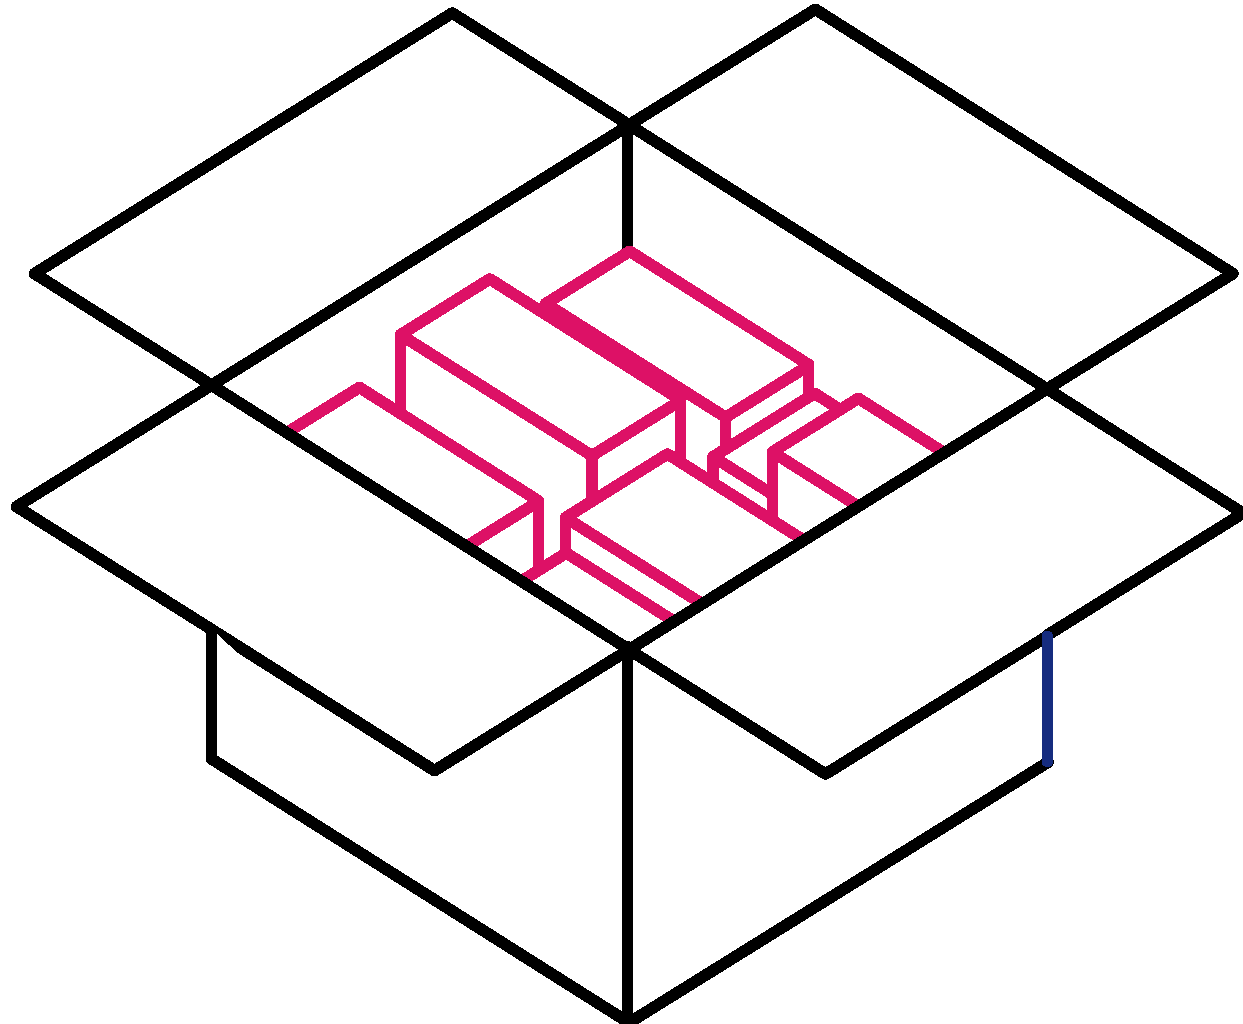
\includegraphics[height=20pt]{../assets/box.pdf}}
\rhead{} %Kopfzeile rechts
\lfoot{} %Fußzeile links
\cfoot{} %Fußzeile mitte
\rfoot{} %Fußzeile rechts
\makeatother


\newcommand{\changefont}{%
    \fontsize{9}{11}\selectfont
}

  
%\setlength\headheight{40pt}
%\setlength\footheight{20pt}
%\lfoot{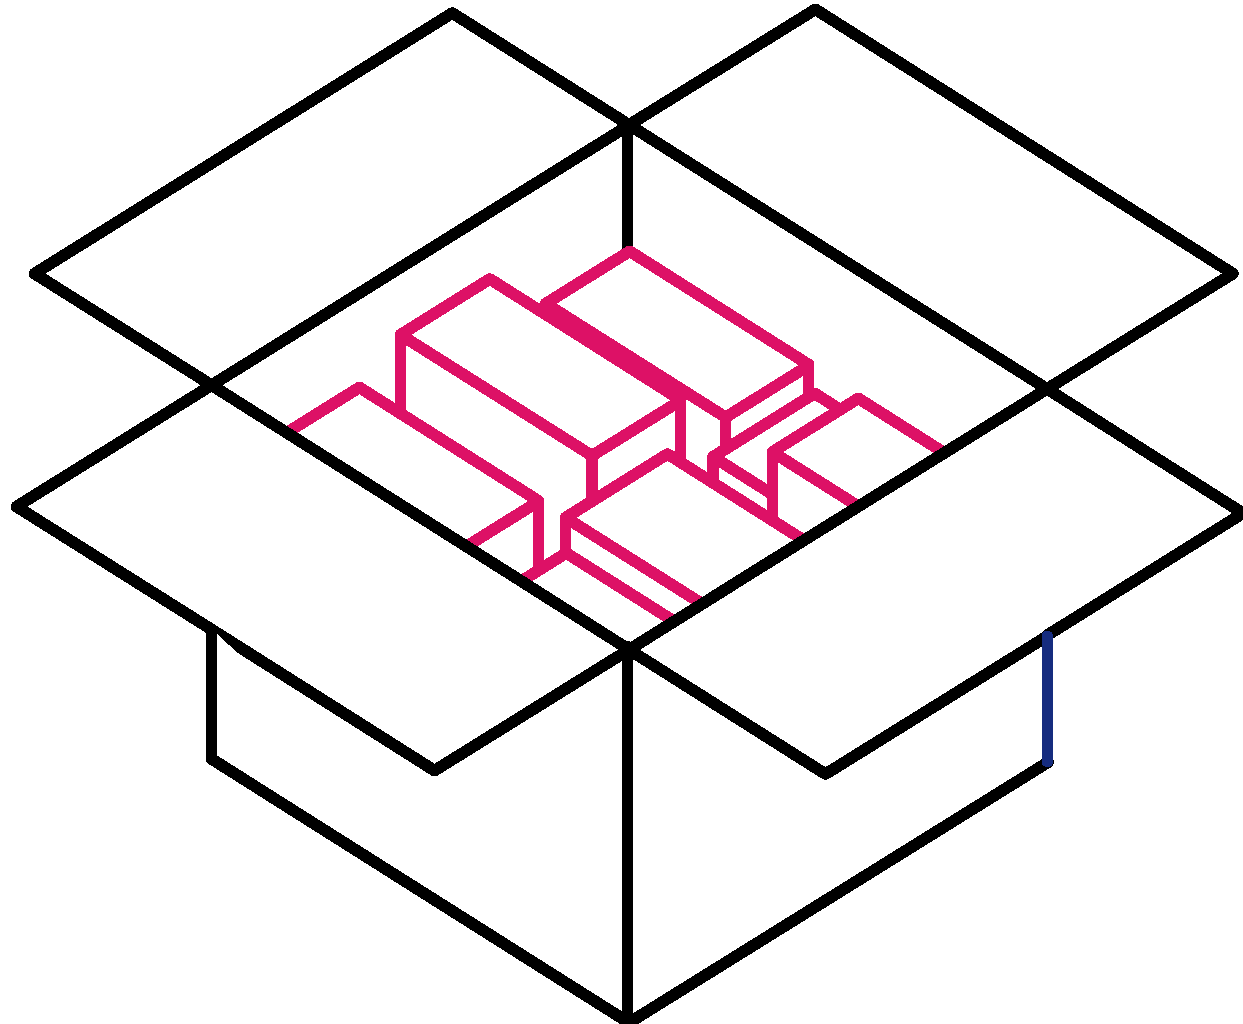
\includegraphics[height=40pt]{../assets/box.pdf}}
\rfoot{\thepage}
\lfoot{\changefont Selbstbericht Medieninformatik\\TH Köln // Institut für Informatik\\ \today}


%\UTF{0192}ndert die Seitennummerierung beim Inhaltsverzeichnis mit eigenem Stil
\renewcommand*{\indexpagestyle}{fancy}
%Verhindert die Seitennummerierung auf den Part-Seiten
\renewcommand*{\partpagestyle}{empty}
%\UTF{0192}ndert die Seitennummerierung bei Chapter mit eigenem Stil
\renewcommand*{\chapterpagestyle}{fancy}

%Abbildungsnummerierung ändern (abhängig von chapter, z.B. Abbildung 1.1)
\renewcommand*{\thefigure}{\thechapter.\arabic{figure}}
%Tabellennummerierung ändern (abhängig von chapter, z.B. Tabelle 1.1)
\renewcommand*{\thetable}{\thechapter.\arabic{table}}

%Paket, um ein Glossar/Abkürzungsverzeichnis anzulegen
\usepackage{nomencl}
\let\abbrev\nomenclature
%Der Name wird in Glossar geändert
\renewcommand{\nomname}{Glossar}
%Definiert die Aufteilung im Glossar zwischen Begriffen und Erläuterung
\setlength{\nomlabelwidth}{.25\hsize}
%Definiert die Punktelinien im Glossar
\renewcommand{\nomlabel}[1]{#1 \dotfill}
\setlength{\nomitemsep}{-\parsep}
%Veranlasst die Erstellung des Glossars
\makenomenclature

%Einrückungen nach Absätzen und Grafiken verhindern
\setlength{\parindent}{0pt}

%Verhindern, dass eine neue Seite für ein einzelnes Wort/Zeile verwendet wird
\clubpenalty = 10000 % schliesst Schusterjungen aus 
\widowpenalty = 10000 % schliesst Hurenkinder aus (keine Beleidigung, sondern wirklich ein Fachbegriff)

%Paket für ein deutsches Literaturverzeichnis
\usepackage{bibgerm}

%Paket für die Verwendung von URLs durch den Befehl \url{}
\usepackage{url}

%Paket für Zeilenabstand (onehalfspace, singlespace)
\usepackage{setspace}

%Paket zur Erzeugung von Anführungszeichen durch \enquote{Text}
\usepackage[ngerman]{babel}
\usepackage[babel, german=quotes]{csquotes}

%Paket für farbigen Text
%black,white,green,red,blue,yellow,cyan,magenta
\usepackage{color}

%Paket für farbigen Hintergrund für Verbatim-Umgebung (Quelltext-Umgebung)
\usepackage{fancyvrb}
\usepackage{verbatim,moreverb}
%Grauton für Quelltext-Umgebung definieren 80% Grau
\definecolor{sourcegray}{gray}{.80}
%Paket für Quelltext-Umgebung
\usepackage{listings}

%Paket für Positionierung der Objekte ohne Float (Verwendungsbsp.: \begin{figure}[H])
\usepackage{float}

%Paket zur Erzeugung von Hyperrefs und PDF Informationen
\usepackage[pdftex,plainpages=false,pdfpagelabels,
            pdftitle={Bachelorarbeit},
            pdfauthor={Vorname Nachname}
            ]{hyperref}

% packages
%\usepackage[super, ]{natbib}

\usepackage{pdfpages}

%\usepackage[toc]{glossaries}

\providecommand{\tightlist}{%
  \setlength{\itemsep}{0pt}\setlength{\parskip}{0pt}}

\usepackage{tabularx}
\newcolumntype{L}[1]{>{\raggedright\arraybackslash}p{#1}}
\newcolumntype{C}[1]{>{\centering\arraybackslash}p{#1}}
\newcolumntype{R}[1]{>{\raggedleft\arraybackslash}p{#1}}

% URL
\usepackage{hyperref}

% Sonderzeichen
\usepackage{textcomp}
\usepackage{eurosym}

\usepackage{setspace}
\renewcommand{\baselinestretch}{1.2}
\setlength{\parskip}{1em}

\usepackage[sfdefault,light]{roboto}  %% Option 'sfdefault' only if the base font of the document is to be sans serif


\usepackage{titlesec}
\titleformat{\chapter}[display]
  {\normalfont\sffamily\mdseries\color{m_lila}}
  {\chaptertitlename\ \thechapter}{14pt}{\huge}
\titleformat{\section}
  {\normalfont\sffamily\Large\mdseries\color{m_lila}}
  {\thesection}{1em}{}

\usepackage[T1]{fontenc}


\usepackage[font=footnotesize]{caption}

%\usepackage[toc]{glossaries}
%\makeglossaries





% Footer definieren
%\usepackage{fancyhdr}
\makeatletter
\def\footrule{{
  \vskip-\footruleskip\vskip-\footrulewidth
  \color{\footrulecolor}
  \hrule\@width\headwidth\@height
  \footrulewidth\vskip\footruleskip
}}
\makeatother
\renewcommand{\footrulewidth}{0.1pt}
\newcommand{\footrulecolor}{m_green}



\begin{document}

% seitennummerierung
%\frontmatter
%\setcounter{page}{3}
%\pagenumbering{arabic}

%Titelseite
%%!TEX root = ../PP.tex

\begin{titlepage}

\begin{center}

%Logo der Fachhochschule Köln
\begin{figure}[!ht]
		
\includegraphics[width=0.2\textwidth]{grafiken/logoheader.jpg}
\end{figure}

\vspace{1.3cm}

%Deutscher Titel
\begin{rmfamily}
\textbf{\small „Eine dramatische Entwertung\\kreativer (Audio)Werke hat stattgefunden“ \cite{K01}\\
				Klaus Warstat}\\
\vspace{1.7cm}
\textbf{\huge Digitales}\\
\vspace{0.3cm}
\textbf{\huge \textcolor{m_pink}{\textbf{KLANG}}BUCH}\\
\vspace{0.2cm}
\textbf{\small Musik als Erlebnis}\\
\vspace{0.8cm}
\LARGE Konzeption eines Leitfadens zu Interaktionen und Inhalten eines digitalen Klang-Buchs
\normalsize
\end{rmfamily}


\vspace{1cm}

%Bachelorarbeit 
\begin{LARGE}
\begin{scshape}
\textbf{\huge Bachelorarbeit}\\[0.5em]
\end{scshape}
\end{LARGE}

\vspace{0.7cm}

%im Studiengang...
\begin{large}
vorgelegt an der Technischen Hochschule Köln\\ 
\vspace{0.2cm}
Campus Gummersbach
\end{large}

\vspace{0.7cm}

%ausgearbeitet von...
\begin{large}
ausgearbeitet von\\ 
\vspace{0.2cm}
\begin{LARGE}
Sahrah El ghammaz\\
\end{LARGE}
\end{large}


\vspace{0.4cm}

%im Studiengang...
\begin{large}
im Studiengang\\ 
\vspace{0.2cm}
\textsc{Medieninformatik}
\end{large}

\vspace{0.6cm}

%Autor der Bachelorarbeit und die Prüfer
\begin{tabular}{rl}
        Erster Prüfer:  &  Prof. Dr. Köhler\\
        %Betreuer:  &  Prof. Dr. Lutz Köhler\\
       							    &  \small Technische Hochschule Köln \\[1.0em]
       Zweiter Prüfer:  &  Prof. Kornacher\\
       							    &  \small Technische Hochschule Köln
\end{tabular}

\vspace{0.6cm}

%Ort, Monat der Abgabe
\begin{large}
Marienheide, September 2015
\end{large}

\end{center}



\end{titlepage}

%\onehalfspacing

%%!TEX root = ../PP.tex

%TODO: 

% \gls{label}
% \glspl{}	PLURAL
% \GLS{}		UPPER case
% \glslink{<label>}{<alternate text>}

%Eintrag ins Glossar
\newglossaryentry{remix}{name=Remix,description={ist eine Version eines Musikstücks auf Basis des Originals}}
\newglossaryentry{clip}{name=Clip,description={s. Videoclip}}
\newglossaryentry{videoclip}{name=Videoclip,description={bezeichnet einen kurzes Video}}
\newglossaryentry{song}{name=Song,description={bezeichnet ein Musikstück}}
\newglossaryentry{responsive}{name=Responsive,description={ist ein Ausdruck aus der Webentwicklung. Responsive Webdesign bedeutet, dass sich das Layout einer Website auf unterschiedlichen Endgeräten anpasst.}}
\newglossaryentry{onepager}{name=Onepager,description={bezeichnet Webseiten, die aus einer einzigen HTML-Seite bestehen.}}
\newglossaryentry{crowdfunding}{name=Crowdfunding,description={Crowdfunding ist eine Form der Finanzierung (’funding’) durch eine Menge (’crowd’) von Internetnutzern."\cite{crowd}}}
\newglossaryentry{button}{name=Button,description={ist eine Schaltfläche, ein Bedienelement}}
\newglossaryentry{artwork}{name=Artwork,description={bezeichnet hier das beiliegende Druckwerk eines Albums, auch Booklet genannt. Im Weiteren bezeichnet es das grafische Material, das für ein Musikalbum produziert wird}}
\newglossaryentry{booklet}{name=Booklet,description={s. Artwork}}
\newglossaryentry{intro}{name=Intro,description={hier: Einführung in den Videoclip}}
\newglossaryentry{outro}{name=Outro,description={hier: Einführung in den Videoclip}}
\newglossaryentry{loop}{name=Loop,description={ist ein in Schleife laufendes Audiostück. Die Anfang und Ende des Loops können lückenlos aneinander gesetzt werden}}
\newglossaryentry{viral}{name=viral,description={bescheibt die Verbreitung von Inhalten in sozialen Kanälen}}
\newglossaryentry{stylesheet}{name=stylesheet,description={oder auch Stylesheet-Sprache oder Cascading Style Sheet, beschreibt eine Sprache, die das Erscheinungsbild einer Website beschreibt und festlegt.}}










 









%Kurzfassung
%%!TEX root = ../PP.tex

\chapter*{Kurzfassung}

Der Umgang mit und die Wertschätzung von Musik hat sich seit der Schallplatte bis zu den Streamingdiensten der heutigen Zeit stark verändert. Der Gesamtumsatz der Musik hat, seit Einführung der MP3, abgenommen, während der Konsum von Musik angestiegen ist.\cite{Musik2014} Musik ist heutzutage ein allgegenwärtiges, leicht zugängliches Konsumgut. Die abnehmende Wertschätzung ist ein Trend, der von Musikern, Künstlern und Musikfans gleichermaßen als Verlust bewertet wird.\cite{K01}\cite{Lost}\\

Eine Idee, um diesem Trend etwas entgegen zu setzen, ist das Schaffen eines neuen Mediums - das digitale Klangbuch. Das Konzept des digitalen Klangbuchs sieht ein großformatiges, physisches Buch als erweitertes, interaktives \gls{artwork} und sinnliches Gesamtpaket vor. Es soll Musik, Bilder, Grafiken und Informationen zum Musiker / Künstler und zur Musik enthalten und den Hörer / Fan interaktiv einbinden, fesseln und begeistern. Mit dem digitalen Klangbuch sollen mehrere Sinne gleichzeitig angesprochen werden: Der akustische, visuelle und der haptische Sinn.\\

Die Entwicklung des digitalen Klangbuchs ist ein Projekt, das aus vielen Teilprojekten besteht. Eines dieser Teilprojekte wurde im vorangegangen Praxisprojekt mit dem Thema „Konzeption eines erweiterten Buches als Tonträger zur Verknüpfung von Audio und Interaktion zur Aufwertung kreativer Audiowerke“ erarbeitet. Ziel des Praxisprojekt war die Beantwortung der Frage: Was sind geeignete technologische Ansätze um ein digitales Klangbuch zu entwickeln?\\

Die Bachelorarbeit setzt das vorangegangene Praxisprojekt fort.\\
Das digitale Klangbuch und dessen Möglichkeiten sind für außenstehende Personen nicht einfach zu verstehen. Ziel der Bachelorarbeit ist die Beantwortung der folgenden Frage: Wie lassen sich die Möglichkeiten und Grenzen des digitalen Klangbuchs gegenüber Musikern und Künstlern vermitteln? Zur Beantwortung dieser Frage wurden im ersten Schritt die Möglichkeiten und Grenzen des digitalen Klangbuchs erläutert. Daraufhin wurden Darstellungs- und Funktionsmöglichkeiten des Klangbuchs erarbeitet. Im Anschluss wurden Arten von Leitfäden recherchiert. Im nächsten Schritt wurde ein Leitfaden konzipiert und entwickelt: Der Aufbau des Leitfadens wurde diskutiert, Layouts gestaltet, Audiomaterial produziert und \gls{videoclip}s konzipiert, gedreht, montiert und vertont. Im Anschluss wurde ein Videokanal auf YouTube erstellt und eine Webseite entwickelt.\\

Die Arbeit wurde mit einem Fazit und einem Ausblick abgeschlossen.


%\singlespacing

%Inhaltsverzeichnis
%%!TEX root = ../PP.tex

\tableofcontents
%\onehalfspacing

%=== Hauptteil =======================================================
%Seitennummerierung des Hauptteils
\mainmatter
%Nummerierung beginnt beim Hauptteil ab Seite 4(muss angepasst werden)
%\setcounter{page}{7}

\chapter{Leitfaden // Programmakkreditierung // Siegel der Stiftung zur
Akkreditierung von Studiengängen in Deutschland (Akkreditierungsrat)}\label{Leitfaden // Programmakkreditierung // Siegel der Stiftung zur
Akkreditierung von Studiengängen in Deutschland (Akkreditierungsrat)}


\section{Vorschläge für die Bearbeitung und
Gliederung}\label{vorschluxe4ge-fuxfcr-die-bearbeitung-und-gliederung}

Die Durchführung eines Akkreditierungsverfahrens basiert auf der Vorlage
eines sogenannten Selbstberichtes seitens der antragstellenden
Hochschule.

Die Phase der Erstellung dieser Selbstbewertung bietet die Möglichkeit,
interne Qualitätssicherungs- (und Reflexions-)Prozesse zu nutzen, um
relevante Interessenträger einzubeziehen und Verbesserungspotentiale
freizusetzen. Im Idealfall wird das Akkreditierungsverfahren als Projekt
zur Qualitätsentwicklung in der Hochschule genutzt und nicht als formale
Prüfroutine durchlaufen.

Die Erstellung der Selbstbewertung setzt sich aus jeweils zwei Schritten
zusammen:

\begin{enumerate}
\def\labelenumi{\arabic{enumi}.}
\tightlist
\item
  \textbf{Selbstbewertung}: Im Selbstbericht bewertet die Hochschule in
  möglichst komprimierter Form selbst, ob und wie für den zu
  akkreditierenden Studiengang/die zu akkreditierenden Studiengänge die
  einzelnen Kriterien erfüllt sind und welche Besonderheiten ggf. zu
  berücksichtigen sind. Auch Abweichungen von den Kriterien können hier
  erläutert werden.
\end{enumerate}

Der Fokus liegt dabei vorrangig auf einer bewertenden, nicht
deskriptiven Einschätzung, die z.~B. nach Stärken, Schwächen,
Herausforderungen und Lösungen gegliedert sein kann. Die nachstehenden
„Leitfragen`` zu jedem Kriterium sollen dazu \emph{eine Hilfestellung}
bieten.

Die Selbstbewertung ist zugleich ein „Wegweiser`` durch ergänzende
Anhänge. Häufig reichen eine prägnante, kurz gefasste Einschätzung zu
dem jeweiligen Kriterium und ein Verweis auf einen Beleg im Anhang als
Dokumentationsgrundlage für das Akkreditierungsverfahren aus.

Richtet sich der Akkreditierungsantrag auf ein „Cluster`` inhaltlich
verwandter Studiengänge, sollten Informationen, die für alle
Studiengänge des Clusters gleichermaßen gelten, zusammengefasst werden.
Zugleich sollten studiengangspezifische Informationen (z. B. angestrebte
Lernergebnisse, Curriculum etc.) unterscheidbar ausgewiesen sein.

\begin{enumerate}
\def\labelenumi{\arabic{enumi}.}
\tightlist
\item
  \textbf{Evidenzen}: Es ist von zentraler Bedeutung, dass die
  vorgelegten Selbstbewertungen nachvollziehbar dokumentiert und durch
  geeignete Belege („Evidenzen``) untermauert werden. Dazu sollte ein
  Anhang mit entsprechenden Belegen („Evidenzen``) zusammengestellt
  werden. Dieser Anhang sammelt die internen Regelungen, Dokumente,
  quantitativen oder qualitativen Daten und Informationen, die bereits
  in der Hochschule vorliegen -- z. B. weil sie im Zuge der internen
  Qualitätssicherung ohnehin produziert werden und deshalb nicht eigens
  für das Akkreditierungsverfahren erstellt werden müssen. Eine
  \emph{exemplarische} Liste potentieller Nachweise, die nach Bedarf
  ergänzt oder abgeändert werden kann, findet sich als Hilfestellung in
  der nachfolgenden Gliederung der Selbstbewertung.
\end{enumerate}

Es empfiehlt sich, für die Erstellung der Selbstbewertung dieses
Gliederungsschema als Vorlage zu nutzen. Das Schema ist nach den
Akkreditierungskriterien aufgebaut und unterscheidet jeweils zwischen
Leitfragen für die Analyse und Hinweisen zu möglicherweise geeigneten
Evidenzen. Beide sind nicht verbindlich, sondern lediglich als
Hilfestellung gedacht.

Selbstbewertung und Evidenzen können je nach Digitalisierungsgrad des
hochschuleigenen Dokumenten- und Datenmanagements grundsätzlich
elektronisch aufbereitet sein, z.~B. auch Zugänge zu spezifischen
Webseiten, Datenbanken o. ä. enthalten. Je nach Bedarf einzelner
Gutachtergruppen bitten wir im konkreten Fall zusätzlich um die
Papierfassung der Antragsunterlagen, wobei mittelfristig der Übergang
zur ausschließlich elektronischen Dokumentation angestrebt wird.

%

\chapter{Qualifikationsziele des Studiengangskonzeptes}\label{Qualifikationsziele des Studiengangskonzeptes}


Das Studiengangskonzept orientiert sich an Qualifikationszielen. Diese
umfassen fachli-che und überfachliche Aspekte und beziehen sich
insbesondere auf die Bereiche

\begin{itemize}
\item
  wissenschaftliche oder künstlerische Befähigung,
\item
  Befähigung, eine qualifizierte Erwerbstätigkeit aufzunehmen,
\item
  Befähigung zum gesellschaftlichen Engagement
\item
  Persönlichkeitsentwicklung
\end{itemize}

\section{Leitfragen}\label{leitfragen}

\begin{itemize}
\item
  An welcher Stelle sind die jeweils im Kriterium genannten
  Kompetenz-Bereiche im Studiengang nach dem Verständnis der Hochschule
  abgebildet?
\item
  Wie wurde das angestrebte Kompetenzprofil des Studiengangs
  (weiter-)entwickelt (Auslöser, Vorgehen, Beteiligungen)?
\item
  Finden die definierten Kompetenzziele für Absolventen des
  Studienprogramms die Zustimmung von Lehrenden und Studierenden?
\item
  Wurde die Stimmigkeit der Lernziele des Studiengangs in den letzten
  Jahren überprüft? Aus welchen Gründen wurden ggf. Anpassungen
  vorgenommen?
\item
  Gibt es Auffälligkeiten bei den qualitativen oder quantitativen
  Daten/Informationen der Hochschule hinsichtlich der Akzeptanz des
  Kompetenzprofils auf dem Arbeitsmarkt?
\end{itemize}

\section{Mögliche Evidenzen}\label{muxf6gliche-evidenzen}

\begin{itemize}
\item
  Dokumente/Stellen, wo die Ziele und Lernergebnisse verankert u.
  veröffentlicht sind, z.B. Ordnungen, Homepage, Diploma Supplement,
  Studienführer
\item
  Interne Unterlagen, aus denen die Einbeziehung der verschiedenen
  Interessenträger hervorgeht, z.B. Vorgaben, Prozessbeschreibungen,
  Befragungsergebnisse, Protokolle
\item
  Ziele-Module-Matrix
\item
  Modulbeschreibungen, wie sie den Lehrenden und Studierenden zur
  Verfügung stehen
\end{itemize}

%

\chapter{Konzeptionelle Einordnung des Studiengangs in das Studiensystem}\label{Konzeptionelle Einordnung des Studiengangs in das Studiensystem}


Der Studiengang entspricht

(1) den Anforderungen des Qualifikationsrahmens für deutsche
Hochschulabschlüsse vom 21.04.2005 in der jeweils gültigen Fassung,

(2) den Anforderungen der Ländergemeinsamen Strukturvorgaben für die
Akkreditierung von Bachelor- und Masterstudiengängen vom 10.10.2003 in
der jeweils gültigen Fassung,

(3) landesspezifischen Strukturvorgaben für die Akkreditierung von
Bachelor- und Masterstudiengängen,

(4) der verbindlichen Auslegung und Zusammenfassung von (1) bis (3)
durch den Akkreditierungsrat.

\section{Leitfragen}\label{leitfragen}

\begin{itemize}
\item
  Inwieweit sehen die für den Studiengang Verantwortlichen die im
  Kriterium genannten Anforderungen (insbesondere ländergemeinsame und
  ggf. landesspezifische Strukturvorgaben) eingehalten? Wo sieht die
  Hochschule Abweichungen und wie sind diese begründet?
\item
  Auf welcher Berechnungsgrundlage fußt die Zuordnung von Kreditpunkten
  zu einzelnen Modulen?
\item
  Sind alle verbindlich vorgeschriebenen Studienbestandteile
  (einschließlich praktischer Studienphasen) kreditiert? Wenn nein,
  warum nicht?
\item
  Sind bei der Vergabe von Abschlusszeugnis und Diploma Supplement an
  die Studierenden Probleme bekannt geworden? Wenn ja, wie wurde darauf
  reagiert?
\end{itemize}

\section{Mögliche Evidenzen}\label{muxf6gliche-evidenzen}

\begin{itemize}
\item
  Studien-/Prüfungsordnung bzw. Zugangssatzung
\item
  Falls nicht in Ordnungen enthalten, ergänzende Dokumente, die
  Studienstruktur und -dauer, ggf. Studiengangsprofile, ggf. Einordnung
  in konsekutive oder weiterbildende Masterstudiengänge, Abschlüsse und
  Abschlussbezeichnungen belegen
\item
  Modulbeschreibungen, wie sie den Lehrenden und Studierenden zur
  Verfügung stehen
\item
  Dokumente, in denen Studienverläufe und deren Organisation geregelt
  sind (z.~B. Studienverlaufspläne)
\item
  Dokumente, die die Kreditpunktezuordnung hochschulweit /
  studiengangbezogen regeln
\item
  exemplarisches Zeugnis je Studiengang
\item
  exemplarisches Diploma Supplement je Studiengang
\item
  exemplarisches Transcript of Records je Studiengang
\end{itemize}

%

\chapter{Studiengangskonzept}\label{Studiengangskonzept}


Das Studiengangskonzept umfasst die Vermittlung von Fachwissen und
fachübergreifendem Wissen sowie von fachlichen, methodischen und
generischen Kompetenzen.

Es ist in der Kombination der einzelnen Module stimmig im Hinblick auf
formulierte Qualifikationsziele aufgebaut und sieht adäquate Lehr- und
Lernformen vor. Gegebenenfalls vorgesehene Praxisanteile werden so
ausgestaltet, dass Leistungspunkte (ECTS) erworben werden können.

Es legt die Zugangsvoraussetzungen und gegebenenfalls ein adäquates
Auswahlverfahren fest sowie Anerkennungsregeln für an anderen
Hochschulen erbrachte Leistungen gemäß der Lissabon Konvention und
außerhochschulisch erbrachte Leistungen. Dabei werden Regelungen zum
Nachteilsausgleich für Studierende mit Behinderung getroffen.
Gegebenenfalls vorgesehene Mobilitätsfenster werden curricular
eingebunden.

Die Studienorganisation gewährleistet die Umsetzung des
Studiengangskonzeptes.

\section{Leitfragen}\label{leitfragen}

\begin{itemize}
\item
  Welchen Beitrag leistet das Curriculum/leisten die einzelnen Module
  aus Sicht der für den Studiengang Verantwortlichen und Beteiligten zum
  Erreichen des angestrebten Kompetenzprofils?
\item
  Hat sich im Zuge eines Abgleichs von angestrebtem Kompetenzprofil und
  Curriculum in den letzten Jahren Anpassungsbedarf ergeben? Welche
  Gründe gab es dafür? Wie wurde reagiert?
\item
  Wie wird erreicht, dass die Module in sich stimmig sind, zueinander
  passen und wo nötig aufeinander aufbauen? Wie reagieren die für einen
  Studiengang Verantwortlichen, wenn einzelne Module sich nicht (mehr)
  in das Gesamtkonzept des Studiengangs einfügen?
\item
  Woran erkennen die für den Studiengang Verantwortlichen, dass die
  Module eines Studiengangs \emph{in ihrer Gesamtheit} das angestrebte
  akademische Niveau tragen?
\item
  Inwieweit tragen die angebotenen Wahlmöglichkeiten im Studiengang zum
  Erreichen des angestrebten Kompetenzprofils bei?
\item
  Woran erkennen die Lehrenden und die für den Studiengang
  Verantwortlichen, dass die gewählten didaktischen Instrumente und
  Methoden das Erreichen der Lernergebnisse des Studiengangs
  unterstützen?
\item
  Können alle Lehrenden die ihrer Meinung nach idealen didaktischen
  Instrumente und Methoden einsetzen? Wenn nein, warum nicht?
\item
  Welche Elemente unterstützen das eigenständige wissenschaftliche
  Arbeiten von Studierenden?
\item
  Erfüllen die ggf. in einem Studiengang vorgesehenen Praxisphasen die
  Erwartungen im Hinblick auf die angestrebten Lernergebnisse?
\item
  Welchen Prinzipien folgt die Hochschule im Umgang mit extern
  erworbenen Leistungen von Studierenden?
\end{itemize}

\section{Mögliche Evidenzen}\label{muxf6gliche-evidenzen}

\begin{itemize}
\item
  Curriculare Übersicht/Studienverlaufsplan, aus der/dem Semesterlage,
  Umfang und studentische Arbeitslast der Module pro Semester
  hervorgehen (ggf. mit Veröffentlichungsort wie z.~B. Homepage,
  Studienführer, Studien- bzw. Prüfungsordnungen) bzw. Dokumente, in
  denen Studienverläufe und deren Organisation geregelt sind
\item
  Dokumente, aus denen die geltenden Regelungen zur
  (Auslands-)Mobilität, Praxisphasen und Anerkennung von an anderen
  Hochschulen / außerhalb der Hochschule erbrachte Leistungen erkennbar
  sind
\item
  Ziele-Module-Matrix
\item
  Modulbeschreibungen, wie sie den Lehrenden und Studierenden zur
  Verfügung stehen
\item
  Dokumente aus dem täglichen Gebrauch an der Hochschule, aus denen das
  vorhandene Didaktik-Konzept hervorgeht
\item
  Einschlägige Ergebnisse interner Befragungen und Evaluationen
\item
  Ggf. Daten zur (Auslands-)Mobilität von Studierenden und zu
  Praxiseinsätzen von Studierenden
\item
  Informationen über die Profile der Bewerber und der zugelassenen
  Studierenden
\end{itemize}

%

\chapter{Studierbarkeit}\label{Studierbarkeit}


Die Studierbarkeit des Studiengangs wird gewährleistet durch:

\begin{itemize}
\item
  die Berücksichtigung der erwarteten Eingangsqualifikationen,
\item
  eine geeignete Studienplangestaltung
\item
  die auf Plausibilität hin überprüfte (bzw. im Falle der
  Erstakkreditierung nach Er-fahrungswerten geschätzte) Angabe der
  studentischen Arbeitsbelastung,
\item
  eine adäquate und belastungsangemessene Prüfungsdichte und
  -organisation,
\item
  entsprechende Betreuungsangebote sowie
\item
  eine fachliche und überfachliche Studienberatung.
\end{itemize}

Die Belange von Studierenden mit Behinderung werden berücksichtigt.

\section{Leitfragen}\label{leitfragen}

\begin{itemize}
\item
  Woran erkennen die Verantwortlichen, dass die (formalen und
  fachlich-inhaltlichen) Zugangskriterien das Erreichen des angestrebten
  Kompetenzprofils unterstützen?
\item
  Ggf.: Wie wurde reagiert, wenn die Zugangsregelungen diesen Zweck aus
  Sicht der für den Studiengang Verantwortlichen nicht erfüllt haben?
\item
  Wie schätzen die für den Studiengang Verantwortlichen und daran
  Beteiligten~-- einschließlich der Studierenden -- die studentische
  Arbeitsbelastung ein? Welche Probleme treten auf? Was wird zu deren
  Lösung unternommen?
\item
  Sind hinsichtlich des Studienabschlusses in der vorgesehenen Zeit in
  den vergangenen Jahren Probleme aufgetreten? Wenn ja, welche? Wie
  wurden sie behandelt?
\item
  Inwieweit sind individuelle Mobilitätsfenster für Studierende im
  Studienverlauf realisierbar? Welche Probleme gibt es? Wie wurde darauf
  reagiert?
\item
  Welche Auswirkungen auf die Studierbarkeit haben die vorhandenen
  (prüfungsrelevanten) Regelungen zu Wiederholungsmöglichkeiten,
  Nachteilsausgleich bei Behinderung, Nichterscheinen im Krankheitsfall
  etc.?
\item
  Gab es Fälle, in denen sich die konkrete Prüfungsorganisation (z.~B.
  Terminierung der Prüfungen, Korrekturzeiten) nachteilig auf den
  Studienverlauf ausgewirkt haben? Wenn ja, welche Konsequenzen wurden
  gezogen?
\item
  Welche der vorhandenen Betreuungs- und Beratungsangebote für
  Studierende halten die für den Studiengang Verantwortlichen und
  Beteiligten -- einschließlich der Studierenden -- für besonders
  effektiv im Hinblick auf den Studienerfolg?
\item
  Welche Betreuungs- und Beratungsangebote für Studierende vermissen die
  für den Studiengang Verantwortlichen und Beteiligten -- einschließlich
  der Studierenden? Warum werden sie nicht realisiert?
\item
  Inwieweit werden Belange von Studierenden mit Behinderung
  berücksichtigt?
\end{itemize}

\section{Mögliche Evidenzen}\label{muxf6gliche-evidenzen}

\begin{itemize}
\item
  Ggf. Zugangssatzung sowie Informationen über die
  Studiengangsvoraussetzungen auf Webseiten, in Studienführern etc.
\item
  Einschlägige Ergebnisse interner Erhebungen und Evaluationen -- ggf.
  Daten zur studentischen Arbeitslast
\item
  Studienverlaufsplan, aus der/dem Semesterlage, Umfang und studentische
  Arbeitslast der Module pro Semester hervorgehen (ggf. mit
  Veröffentlichungsort wie z.~B. Homepage, Studienführer, Studien- bzw.
  Prüfungsordnungen) bzw. Dokumente, in denen Studienverläufe und deren
  Organisation geregelt sind
\item
  Dokumente, aus denen die geltenden Regelungen zur
  (Auslands-)Mobilität, Praxisphasen und Anerkennung von an anderen
  Hochschulen / außerhalb der Hochschule erbrachten Leistungen erkennbar
  sind
\item
  Dokumente aus dem täglichen Gebrauch an der Hochschule, aus denen das
  vorhandene Beratungs- und Betreuungskonzept hervorgeht
\item
  (statistische) Daten zu Studienverläufen
\item
  Ggf. Daten zur (Auslands-)Mobilität von Studierenden und zu
  Praxiseinsätzen von Studierenden
\item
  Ggf. weitere einschlägige Ergebnisse interner Befragungen und
  Evaluationen (auch Auffälligkeiten hinsichtlich der Wirkung von ggf.
  vorhandenen Maßnahmen zur Vermeidung von Ungleichbehandlungen in der
  Hochschule)
\end{itemize}

%

\chapter{Studiengangsbezogene Kooperationen}\label{Studiengangsbezogene Kooperationen}


Beteiligt oder beauftragt die Hochschule andere Organisationen mit der
Durchführung von Teilen des Studiengangs, gewährleistet sie die
Umsetzung und die Qualität des Studiengangskonzeptes. Umfang und Art
bestehender Kooperationen mit anderen Hochschulen, Unternehmen und
sonstigen Einrichtungen sind beschrieben und die der Kooperation zu
Grunde liegenden Vereinbarungen dokumentiert.

\section{Leitfragen}\label{leitfragen}

\begin{itemize}
\tightlist
\item
  Funktionieren die hochschulinternen und hochschulexternen
  Kooperationen aus Sicht der für den Studiengang Verantwortlichen?
\end{itemize}

\section{Mögliche Evidenzen}\label{muxf6gliche-evidenzen}

\begin{itemize}
\tightlist
\item
  Kooperationsverträge, Regeln für interne/externe Kooperationen
\end{itemize}

%



\chapter{Ausstattung}\label{Ausstattung}


Die adäquate Durchführung des Studiengangs ist hinsichtlich der
qualitativen und quantitativen personellen, sächlichen und räumlichen
Ausstattung gesichert. Dabei werden Verflechtungen mit anderen
Studiengängen berücksichtigt. Maßnahmen zur Personalentwicklung und
-qualifizierung sind vorhanden.

\section{Leitfragen}\label{leitfragen}

\begin{itemize}
\item
  Auf welche Weise stellen die für den Studiengang Verantwortlichen
  fest, dass Umfang und fachliche Qualifikation des Lehrpersonals für
  Lehre und Betreuung ausreichen?
\item
  Wie zufrieden sind die am Studiengang Beteiligten mit den Ressourcen
  für Lehre, Betreuung und Administration?
\item
  Wie reagieren die für den Studiengang Verantwortlichen auf auftretende
  Probleme und Engpässe?
\item
  Woran wird die Qualität von ggf. eingesetzten Lehrbeauftragten fest
  gemacht?
\item
  Inwieweit sind Forschungs- und Entwicklungstätigkeiten der Lehrenden
  der Studiengangsentwicklung förderlich?
\item
  Wer ist für die fachliche und didaktische Weiterentwicklung der
  Lehrenden verantwortlich?
\item
  Woran erkennen die Verantwortlichen, dass Weiterbildungsmaßnahmen
  erwünscht oder erforderlich sind?
\item
  Wie zufrieden sind die am Studiengang Beteiligten mit der sächlichen
  Ausstattung?
\item
  Wie reagieren die für den Studiengang Verantwortlichen auf Engpässe in
  der Ausstattung?
\end{itemize}

\section{Mögliche Evidenzen}\label{muxf6gliche-evidenzen}

\begin{itemize}
\item
  Beschreibung des Personals
\item
  Dokument aus dem täglichen Gebrauch der Hochschule, aus dem die
  ausreichende Lehrkapazität hervorgeht
\item
  Anzahl der Studierenden
\item
  Darstellung des didaktischen Weiterbildungsangebotes (ggf. Verweis auf
  Webseite) und von Maßnahmen zur Unterstützung der Lehrenden bei dessen
  Inanspruchnahme
\item
  Daten zu wahrgenommenen Weiterbildungsaktivitäten, z.~B.
  Forschungssemester, Gastprofessuren, Seminare, Tagungen, Workshops
\item
  (Kurz-)Darstellung der studiengangsbezogenen Forschungsaktivitäten
\item
  Dokumente aus dem täglichen Gebrauch der Hochschule, in denen die
  Ausstattung dargestellt wird, z.B. Laborhandbücher, Inventarlisten,
  Finanzpläne
\end{itemize}

%

\chapter{Transparenz und Dokumentation}\label{Transparenz und Dokumentation}


Studiengang, Studienverlauf, Prüfungsanforderungen und
Zugangsvoraussetzungen ein-schließlich der Nachteilsausgleichsregelungen
für Studierende mit Behinderung sind dokumentiert und veröffentlicht.

\section{Leitfragen}\label{leitfragen}

\begin{itemize}
\item
  Wie wird sichergestellt, dass inländische und ausländische Studierende
  ihre Rechte und Pflichten kennen?
\item
  Wer hat die Entscheidungsbefugnis über welche Dokumente?
\end{itemize}

\section{Mögliche Evidenzen}\label{muxf6gliche-evidenzen}

\begin{itemize}
\item
  Vorlage aller relevanten Regelungen zu Studienverlauf, Zugang,
  Studienabschluss, Prüfungen, Qualitätssicherung etc., mit Angabe zum
  Status der Verbindlichkeit
\item
  Verweis auf die Stelle, an der diese veröffentlicht sind, z.B.
  Webseiten
\end{itemize}

%

\chapter{Qualitätssicherung und Weiterentwicklung}\label{Qualitätssicherung und Weiterentwicklung}


Ergebnisse des hochschulinternen Qualitätsmanagements werden bei den
Weiterentwicklungen des Studienganges berücksichtigt. Dabei
berücksichtigt die Hochschule Evaluationsergebnisse, Untersuchungen der
studentischen Arbeitsbelastung, des Studienerfolgs und des
Absolventenverbleibs.

\section{Leitfragen}\label{leitfragen}

\begin{itemize}
\item
  Welche Maßnahmen zur Qualitätsverbesserung in und von Studiengängen
  sind in den zurückliegenden Jahren ergriffen worden?
\item
  Welche Elemente der internen Qualitätskontrolle erweisen sich als
  besonders nützlich für kontinuierliche Verbesserungen in einem
  Studiengang?
\item
  Inwieweit findet der Aspekt „Lernergebnisorientierung`` bei der
  Konzeption und in der Praxis der Qualitätssicherungsinstrumente für
  einen Studiengang Berücksichtigung?
\item
  Wie bewerten Studierende die interne Qualitätskontrolle
  und~-entwicklung ihrer Studiengänge hinsichtlich

  \begin{itemize}
  \item
    ihrer Beteiligung?
  \item
    der Auswirkungen auf ihr Studium?
  \end{itemize}
\item
  Wie bewerten Lehrende und die Leitungsebenen die interne
  Qualitätskontrolle und -entwicklung ihrer Studiengänge hinsichtlich

  \begin{itemize}
  \item
    ihrer Beteiligung?
  \item
    der Unterstützung bei der Lösung von Problemen und Verbesserungen in
    der Lehre?
  \end{itemize}
\end{itemize}

\section{Mögliche Evidenzen}\label{muxf6gliche-evidenzen}

\begin{itemize}
\item
  Interne Regelwerke zum Qualitätsmanagement (Evaluationsordnungen u.ä.)
\item
  Exemplarisches Informationsmaterial über das Qualitätsmanagement und
  seine Ergebnisse, das die Hochschule regelmäßig für die Kommunikation
  nach innen und außen nutzt (z.~B. Link zu spezifischen Webseiten,
  Berichte, Flyer)
\item
  Quantitative und qualitative Daten aus Befragungen, Statistiken zum
  Studienverlauf, Absolventenzahlen und -verbleib u.ä.
\end{itemize}

%



\chapter{Geschlechtergerechtigkeit und Chancengleichheit}\label{Geschlechtergerechtigkeit und Chancengleichheit}


Auf der Ebene des Studiengangs werden die Konzepte der Hochschule zur
Geschlechtergerechtigkeit und zur Förderung der Chancengleichheit von
Studierenden in besonderen Lebenslagen wie beispielsweise Studierende
mit gesundheitlichen Beeinträchtigungen, Studierende mit Kindern,
ausländische Studierende, Studierende mit Migrationshintergrund und/oder
aus sogenannten bildungsfernen Schichten umgesetzt.

\section{Leitfragen}\label{leitfragen}

\begin{itemize}
\tightlist
\item
  Liegen Konzepte der Hochschule zur Geschlechtergerechtigkeit und zur
  Förderung der Chancengleichheit von Studierenden in besonderen
  Lebenslagen vor? Wenn ja welche?
\end{itemize}

\section{Mögliche Evidenzen}\label{muxf6gliche-evidenzen}

\begin{itemize}
\tightlist
\item
  Einschlägige Dokumente aus dem alltäglichen Gebrauch der Hochschule,
  die die ggf. vorhandenen Konzepte und Maßnahmen zeigen
\end{itemize}

%



%%!TEX root = ../PP.tex

\newcommand{\fFunktionen}{040_funktionen}

\part{Der Leitfaden}

\textbf{Der Leitfaden - Beschreibung}\\
Dieser Teil erläutert die Möglichkeiten und Grenzen des digitalen Klangbuchs. Es werden Darstellungsmöglichkeiten und Funktionen erarbeitet. Arten von Leitfäden werden diskutiert und ein Leitfaden konzipiert und umgesetzt.

%!TEX root = ../PP.tex

%TODO: 

\chapter{Möglichkeiten und Grenzen des digitalen Klangbuchs}\label{moeglichkeiten}

Bevor ein Leitfaden und Funktionen für das digitale Klangbuch entwickelt werden können, müssen zuvor die Möglichkeiten und Grenzen des digitalen Klangbuchs erläutert werden. Im Folgenden wird das digitale Klangbuch mit seinen technischen Möglichkeiten und Grenzen kurz skizziert.


%%%%%%%%%%%%
%%%%%%%%%%%%

\section{Technik im digitalen Klangbuch}

Im Praxisprojekt wurden unterschiedliche Realisierungsansätze vorgestellt. Die Ansätze präsentierten dabei verschiedene Technologien und Möglichkeiten zum Aufbau des Buches. Um den Rahmen der Bachelorarbeit nicht zu sprengen, beschränkt sie sich auf folgende Technologien und Hilfsmittel, die bei der Funktionsentwicklung und der Entwicklung des Leitfadens im digitalen Klangbuch eingesetzt werden:


\begin{itemize}
\item{Leitende Tinte}
\item{Leitender Kleber}
\item{Gedruckte Elektronik}
\item{SMD-LEDs}
\end{itemize}

\textbf{Leitende Tinte} ist eine Flüssigkeit, mit der sich funktionierende Stromkreise auf Papier zeichnen und drucken lassen. Aufgrund des körpereigenen Widerstands ist die Tinte berührungsempfindlich. Dadurch lassen sich Bedienelemente direkt auf das Papier drucken.\\

Unter \textbf{gedruckte Elektronik} versteht man elektronische Bauteile, die über ein spezielles Verfahren auf ein Trägermaterial aufgedruckt werden können. Ein zentraler Ansatz im digitalen Klangbuch ist die Erkennung der Seite, auf der sich der Hörer gerade befindet. Dadurch lassen sich Funktionen, die nur auf einer bestimmten Seite möglich sind, steuern. Z. B. das automatische Starten eines Songs, sobald eine spezielle Seite umgeblättert wird. Ein gedruckter Sensor ist für die Seitenerkennung notwendig. Der Sensor ist nicht sichtbar zwischen zwei Seiten eingebettet und taucht deshalb nicht in den Skizzen der Funktionsbeschreibungen auf.\\


\textbf{Leitender Kleber} ist ein Klebstoff, der Strom leitet. Damit lassen sich Elemente, die an einen Stromkreis angeschlossen werden müssen, über den Klebstoff integrieren, z. B. SMD-LEDs. Der Kleber wiederum wird mit leitender Tinte verbunden.\\


\textbf{SMD-LEDs} sind winzig kleine LEDs, die ohne Drähte auskommen. Sie können mit dem leitenden Kleber direkt auf das Papier des Klangbuchs aufgeklebt werden. Die kleinste Bauform misst eine Größe von 1,0 x 0,5 x 0,45 mm.\\


%%%%%%%%%%%%


\section{Aufbau Digitales Klangbuch}
In Abbildung \ref{fig:aufbauBuch} ist der Aufbau des digitalen Klangbuchs skizziert: Im hinteren Buchdeckel ist die Technik zur Steuerung eingebettet (1). Der Buchrücken (3) ist mit den Komponenten im Buchdeckel verbunden. Auf den einzelnen Seiten des Buches können mit leitender Tinte berührungsempfindliche Elemente (2.1) gedruckt und mit leitendem Kleber SMD-LEDs (2.2) integriert werden. Jede SMD-LED und jedes berührungsempfindliche Element muss mit leitender Tinte mit dem Buchrücken verbunden werden.


\begin{figure}[H]
\centering
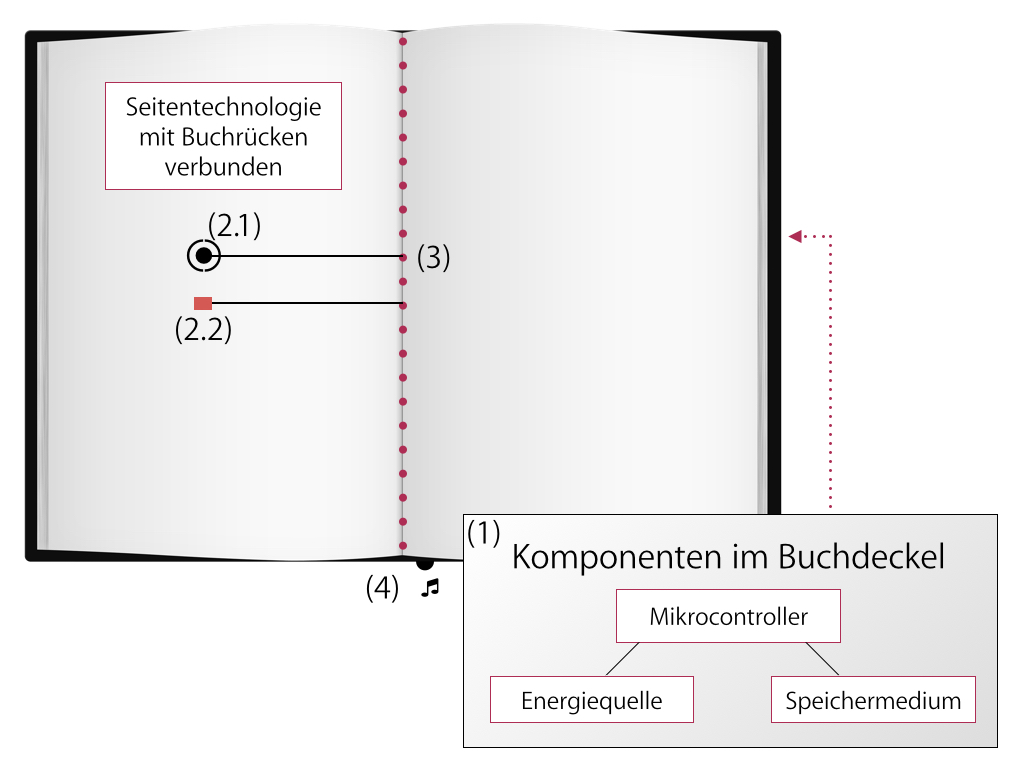
\includegraphics[width=1.0\textwidth]{grafiken/aufbau-klangbuch.jpg}
\caption{Aufbau des digitalen Klangbuchs: (1) Technik im Buchdeckel, (2.1) berührungsempfindliches Element, (2.2) SMD-LED, (3) Buchrücken, (4) Audioausgang }
\label{fig:aufbauBuch}
\end{figure}


\section{Möglichkeiten \& Grenzen}

\subsection{Möglichkeiten}
Durch den Einsatz der zuvor beschriebenen Technik, ist es möglich Audiodaten abzuspielen, SMD-LEDs anzusteuern und Interaktionen auszuwerten (Berührung eines berührungsempfindlichen Elements). Die Auswertung der Interaktion kann für den Hörer in zwei Formen sichtbar gemacht werden:\\
1. Eine Interaktion bewirkt eine eine akustische Veränderung: ein Klang ertönt oder verstummt (z. B. wird ein Song beim Berühren eines bestimmten Elements gestartet).\\
2. Eine Interaktion bewirkt eine visuelle Veränderung: eine oder mehrere SMD-LEDs beginnen zu leuchten, verdunkeln, blinken oder ändern ihren Farbwert.

\subsection{Grenzen}
Berührungsempfindliche Elemente werden mit spezielle, leitende Tinte auf die Seiten des Buches gedruckt. Diese Elemente und jede integrierte SMD-LED werden durch Linien aus gedruckter leitender Tinte mit dem Buchrücken verbunden. Bei der Erstellung der Layouts müssen diese Elemente und Linien berücksichtigt werden. Dabei ist auch zu beachten, dass die Linien ebenfalls auf Berührung reagieren und sie sich auch gegenseitig nicht berühren dürfen.



%%%%%%%%%%%%%%%%%%%%%%%%%%%%%%%%%%%%%%%%%%%%%%%%%%%%%%%%%%%%%%%%%%%%%%%%%%%%%%%%%%%%%%%%%%%%%%%%
%%%%%%%%%%%%%%%%%%%%%%%%%%%%%%%%%%%%%%%%%%%%%%%%%%%%%%%%%%%%%%%%%%%%%%%%%%%%%%%%%%%%%%%%%%%%%%%%
%%%%%%%%%%%%%%%%%%%%%%%%%%%%%%%%%%%%%%%%%%%%%%%%%%%%%%%%%%%%%%%%%%%%%%%%%%%%%%%%%%%%%%%%%%%%%%%%
%%%%%%%%%%%%%%%%%%%%%%%%%%%%%%%%%%%%%%%%%%%%%%%%%%%%%%%%%%%%%%%%%%%%%%%%%%%%%%%%%%%%%%%%%%%%%%%%
%%%%%%%%%%%%%%%%%%%%%%%%%%%%%%%%%%%%%%%%%%%%%%%%%%%%%%%%%%%%%%%%%%%%%%%%%%%%%%%%%%%%%%%%%%%%%%%%


\chapter{Darstellungs- und Funktionsmöglichkeiten}\label{funktionen}

Das digitale Klangbuch spricht den haptischen, visuellen und akustischen Sinn an. Im Folgenden werden Ideen und Funktionen entwickelt. Diese werden in folgende Bereiche unterteilt: Interaktion (haptische Wahrnehmung), Darstellungsmöglichkeiten (visuelle Wahrnehmung) und Akustik (auditive Wahrnehmung).

%%%%%%%%%%%%
%%%%%%%%%%%%
%%%%%%%%%%%%

\section{Interaktion}
Das digitale Klangbuch ermöglicht es dem Hörer interaktiv mit dem Buch und dessen Inhalte zu agieren.

\subsection{Berührungsempfindliche Elemente}
Elemente, die mit leitender Tinte gedruckt und mit dem Buchrücken verbunden wurden, sind berührungsempfindlich. Bei Berührung können sie eine Funktion auslösen, z. B. das Starten eines Songs. Durch logische Verknüpfungen ist es auch möglich berührungsempfindliche Elemente miteinander zu verketten. Ein Beispiel: Berührung von Element A löst Funktion a aus. Berührung Element B, löst Funktion b aus. Berührung von Element A und B zu gleicher Zeit, löst Funktion c aus.

\subsection{Umblättern einer Seite}
Die Seiten des digitalen Klangbuchs sind mit Sensoren ausgestattet. Wird eine Seite umgeblättert, registriert der Sensor auf welcher Seite sich der Hörer befindet. Es kann dann eine Funktion ausgelöst werden, z. B. das Starten eines Songs.


%%%%%%%%%%%%
%%%%%%%%%%%%
%%%%%%%%%%%%

\section{Darstellungsmöglichkeiten}

Im digitalen Klangbuch ist an Inhalten alles möglich, was ein herkömmliches Buch bietet: Raum für Geschichten, Bilder, Illustrationen, Texte, etc. Kombiniert mit der Technik, den Interaktionsmöglichkeiten und der Musik bzw. Audioinhalten, lassen sich unzählige, neuartige Inhalte generieren. Denkbar wären z. B.:

\begin{itemize}
\item Entstehungsgeschichte des Musikers / der Band, begleitet von Musik, Audiokommentaren, etc.
\item Informationen und Geschichten über den Musiker / der Band
\item Bedeutung, die hinter einem ausgewählten Songs steht
\item Entstehungsprozess eines ausgewählten Songs
\item bisherige Veröffentlichungen, \gls{remix}e, etc.
\item Lyriktexte der Songs
\item Fotos des Musikers / der Band
\item Zeichnungen, Bilder, Illustrationen
\end{itemize}

Die Seiten des digitalen Klangbuchs bestehen aus gängigem Fotopapier. Sie können nach Wünschen des Künstlers farbig bedruckt werden. So können Fotos, Grafiken, künstlerische Werke, Texte, etc. auf die Seiten gedruckt werden. Es ist ebenfalls möglich spezielle Techniken aus der Buchkunst zu integrieren, z. B. Pop Up´s\footnote{Pop Up Kunst bezeichnet Elemente, die durch eine besondere Falttechnik räumlich herausspringen (pop up).} (s. Abbildung \ref{fig:Popup}) und diese ebenfalls mit leitender Tinte und SMD-LEDs zu kombinieren (s. Abbildung \ref{fig:PopupLED}.\\


\begin{figure}[H]
\centering
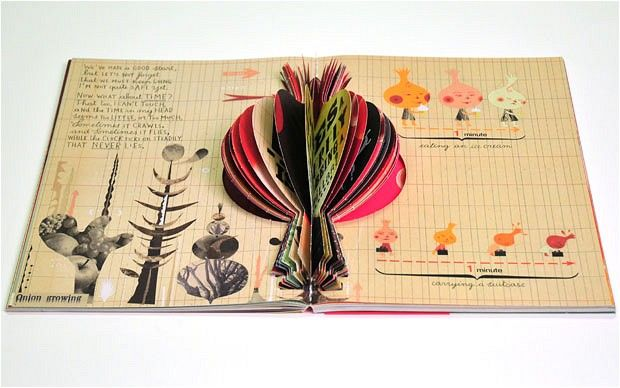
\includegraphics[width=0.8\textwidth]{grafiken/popup.jpg}
\caption{Pop Up Kunst in einem Buch.\\Foto: The Onion’s Great Escape by Sara Fanelli, Portia Webb, \url{http://www.telegraph.co.uk/culture/books/children_sbookreviews/9682987/Books-for-Christmas-childrens-books.html} }
\label{fig:Popup}
\end{figure}


\subsection{Leuchtende Elemente}
Durch eingesetzte SMD-LEDs ist es möglich Veränderungen visuell anzuzeigen und so Informationen zu transportieren. Eine SMD-LED kann blinken, leuchten und die Farbe wechseln. So können z. B. SMD-LEDs auf einer Zeitleiste angeordnet werden, welche dem Hörer durch Blinken anzeigt, an welcher Stelle sich der Song gerade befindet.


\begin{figure}[H]
\centering
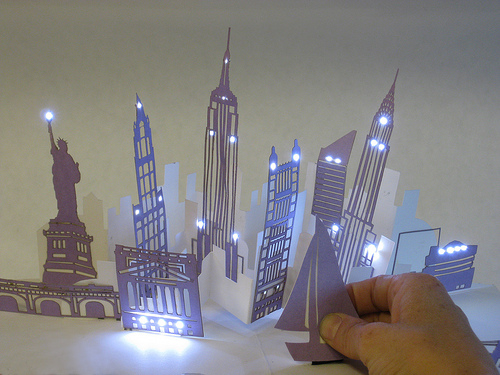
\includegraphics[width=0.5\textwidth]{grafiken/popupled.jpg}
\caption{Pop Up Kunst mit LEDs.\\Foto: Electronic Popables, high-low tech, \url{http://highlowtech.org/?p=5} }
\label{fig:PopupLED}
\end{figure}


\subsection{Grenzen im Layout}
Berührungsempfindliche Elemente werden mit spezieller, leitender, schwarzer Tinte auf die Seiten des Buches gedruckt. Diese Elemente und jede integrierte SMD-LED werden durch Linien aus gedruckter leitender Tinte mit dem Buchrücken verbunden. Bei der Erstellung der Layouts müssen diese Elemente und Linien berücksichtigt werden. Dabei ist auch zu beachten, dass die Linien ebenfalls auf Berührung reagieren und sie sich auch gegenseitig nicht berühren dürfen.

\begin{figure}[H]
\centering

\includegraphics[width=0.8\textwidth]{grafiken/bspklangbuch.png}
\caption{Beispiel Layout eines digitalen Klangbuchs: Berührungsempfindliche Elemente werden mit Linien aus leitender Tinte mit dem Buchrücken verbunden. Die Linien dürfen sich nicht kreuzen.}
\end{figure}




%%%%%%%%%%%%
%%%%%%%%%%%%
%%%%%%%%%%%%

\section{Akustik}
Ein herkömmliches CD-/DVD-/Blueray-Album bietet dem Fan in manchen Fällen auch Bonusmaterial. Das Bonusmaterial ist vor allem auf der CD begrenzt und besteht oft nur aus einem zusätzlichen Song, z. B. ein \gls{remix}. Mit dem digitalen Klangbuch soll das herkömmliches Album um Funktionen und Inhalte erweitert werden. In diesem Kapitel werden Funktionen und Ideen vorgestellt, die vor allem den akustischen Sinn des Fans ansprechen sollen. 


\subsection{Audio abspielen}
Die grundlegendste Funktion ist die Möglichkeit ein Audiostück zu starten, zu stoppen, zu pausieren und die Lautstärke zu regeln.\\


\textbf{Unterschied zum herkömmlichen Album}\\
Der Hörer berührt im digitalen Klangbuch Elemente, die auf eine Papierseite aufgedruckt sind. Dadurch wird der haptische und der auditive Sinn angesprochen.\\

\textbf{Erweiterte Funktionsmöglichkeit}\\
Die Veränderungen können durch SMD-LEDs angezeigt werden, wodurch auch eine visuelle Änderung wahrgenommen werden kann.


%%%%%%%%%%%%


\subsection{Sprachwahl}
Die Gesangsspur eines Songs kann über eine Auswahl in einer anderen Sprache abgespielt werden.\\


\textbf{Unterschied zum herkömmlichen Album}\\
Ein Song, der Gesang oder Sprache enthält, wird für gewöhnlich in einer ausgewählten Sprache gesungen / gesprochen. Selten hat der Hörer die Möglichkeit den Song auch in einer anderen Sprache zu hören. Der KlangKünstler kann dem Hörer eine Auswahl an Spuren in unterschiedlicher Sprache anbieten.\\


\textbf{Weiteres Nutzungsszenario}\\
Dem Hörer kann es möglich sein die Gesangsspur durch eine eigene zu ersetzen.



%%%%%%%%%%%%


\subsection{Interview}
Statt eines Songs, können auch Interviews des KlangKünstler hinterlegt werden.\\


\textbf{Unterschied zum herkömmlichen Album}\\
Im Gegensatz zu einem kleinformatigem \gls{booklet}, können die Interviews im großformatigen digitalen Klangbuch ausführlich grafisch begleitet werden. So kann der Fan zu vielen Details im Interview visuell bedient werden.\\


\textbf{Weiteres Nutzungsszenario}\\
Anhand von SMD-LEDs können visuelle Inhalte des Buches (Bilder, Texte, etc.) passend zu den Stellen des Interviews deutlich gemacht werden.



%%%%%%%%%%%%


\subsection{Equalizer - Presets}
Eine weitere Grundfunktion, die in gängigen Geräten zum Abspielen von Audio enthalten ist, ist ein Equalizer. Er dient dazu um den Klang an die eigenen Wünsche anzupassen: Höhen, Tiefen, etc. Das digitale Klangbuch kann hierzu sogenannte Presets, parametrische Voreinstellungen des Equalizers, anbieten.\\

\textbf{Unterschied zum herkömmlichen Album}\\
Der Hörer berührt im digitalen Klangbuch Elemente, die auf einer Papierseite aufgedruckt sind. Dadurch wird der haptische und der auditive Sinn angesprochen.\\

\textbf{Erweiterte Funktionsmöglichkeit}\\
Die Veränderungen können durch SMD-LEDs angezeigt werden, wodurch auch eine visuelle Änderung wahrgenommen werden kann.


%%%%%%%%%%%%

\subsection{\gls{remix}e}
Der Hörer kann sich zu einem Song verschiedene \gls{remix}e anhören.\\

\textbf{Unterschied zum herkömmlichen Album}\\
Im Gegensatz zu einem kleinformatigem \gls{booklet}, können die \gls{remix}e im großformatigen digitalen Klangbuch ausführlich grafisch begleitet werden.


%%%%%%%%%%%%
%%%%%%%%%%%%
%%%%%%%%%%%%


\subsection{Multitrack}
Multitrack bedeutet zu deutsch "Mehrspur". Es bietet die Möglichkeit einen Song in mehreren, separaten Spuren abzuspielen und diese bei Bedarf einzeln stummzuschalten, auszutauschen oder zu bearbeiten.\\

\textbf{Unterschied zum herkömmlichen Album}\\
Der Hörer hat hier die Möglichkeit einzelne Spuren stumm zu schalten und die Lautstärke der Spuren einzeln zu verändern.\\

\textbf{Erweiterte Funktionsmöglichkeit}\\
Dem Hörer kann es möglich sein eine der Spuren, z. B. die Gesangsspur, durch eine eigene zu ersetzen.


%%%%%%%%%%%%


\subsection{SongKit}
Als SongKit ist in diesem Kontext ein Bausatz zu verstehen, der verschiedene \gls{loop}s einer Klangspur zur Verfügung stellt. Die Idee dahinter ist, ein Musikstück des Albums in seine Spuren zu teilen - beispielsweise in Bass, Drums, Melodie, Gesang - und diese in einer Dauerschleife abspielen zu lassen. Zu jeder Spur gibt es Alternativen, die ausgewählt werden können. So kann der ursprüngliche Song verändert werden.\\


\textbf{Unterschied zum herkömmlichen Album}\\
In der Produktionsphase eines Songs verändert sich der Song von der Idee bis zum fertigen Song. Andere Versionen des Songs, z. B. mit einer anderen Basspur, bekommt der Musikfan nahezu nie zu hören. Durch das SongKit im Klangbuch können diese Versionen integriert werden. Dabei kann der Hörer selbst bestimmen, welche Spuren er zusammen mischt.\\


\textbf{Weiteres Nutzungsszenario}\\
Das SongKit kann unabhängig vom Album eine Auswahl an \gls{loop}s bereit stellen. Das heißt, die \gls{loop}s müssen nicht zwingend einen Bezug zu dem Album oder einem Song haben. Die KlangKünstler können einen Baukasten mit passenden \gls{loop}s zusammen stellen, die der Hörer dann nach seinen Wünschen zu einem Song-\gls{loop} zusammen stellt.



%%%%%%%%%%%%


\subsection{Audiokommentare}
Zu einem Song können Audiokommentare hinterlegt werden, die sich der Hörer bei Bedarf anhören kann. Die Audiokommentare können in einer Timeline, passend zum Song, hinterlegt werden. Aktiviert der Hörer die Audiokommentare, reduziert sich die Lautstärke des bereits laufenden Songs, sodass die entsprechenden Audiokommentare an den passenden Stellen erklingen können. \\


\textbf{Unterschied zum herkömmlichen Album}\\
Audiokommentare sind selten in einem gewöhnlichen Musikalbum zu finden.\\


\textbf{Weiteres Nutzungsszenario}
\begin{itemize}
\item Variation 1: Audiokommentare können über einzelne \gls{button}s individuell gestartet werden.
\item Variation 2: Die Kommentare können als Texte im Buch hinterlegt werden. Erreicht der laufende Song einen Audiokommentar, leuchtet eine dazu platzierte SMD-LED auf. Ein ähnliches Konzept findet sich auf Soundcloud\footnote{Soundcloud ist ein Online-Musikdienst für Musiker zum Anbieten von Audiodateien. Fans können auf der Zeitleiste eines Songs zu jeder Sekunde einen Kommentar hinterlassen.}.
\end{itemize}


%%%%%%%%%%%%


\subsection{Interaktiver Song}
In interaktiven Videos\footnote{Interaktives Videobeispiel: Ink von Colplay\cite{CO}} ist es möglich den Handlungsstrang zu beeinflussen. Der Verlauf eines Songs kann über das digitale Klangbuch ebenfalls durch den Hörer bestimmt werden. Ein Beispiel dazu wird in der Skizze - Abbildung \ref{fig:abb1} veranschaulicht.\\
Beim Öffnen der Seite wird der Song automatisch gestartet. Die Zeitleiste (a) symbolisiert die Länge des Songs. Der Hörer hat nun die Möglichkeit den Verlauf des Songs, während dieser bereits spielt, zu ändern. Dazu wurde der Song in drei Bereiche geteilt (Minute 0:30, 1:30 und 2:30). Diese Bereiche werden im Folgenden "Kapitel" genannt.\\ 

Der Hörer hat die Möglichkeit in jedem Kapitel den Verlauf des Songs zu verändern:
\begin{itemize}
\item Kapitel 1: Der Song kann eine dramatische, eine ruhige oder eine rätselhafte Richtung einschlagen.
\item Kapitel 2: Die Gesangsstimme kann männlich, weiblich oder die eines Kindes sein.
\item Kapitel 3: Das Ende des Songs kann mitbestimmt werden - ein fröhliches, ein zerstörtes oder überhaupt kein Ende, sodass der Song von neuem beginnt.
\end{itemize} 

SMD-LEDs (b) zeigen dem Hörer an, wie lang es ihm möglich ist den Verlauf für dieses Kapitel zu ändern. Solange die SMD-LED in einem der Kapitel leuchtet, kann der Hörer den Verlauf bestimmen.


\begin{figure}[H]
\centering
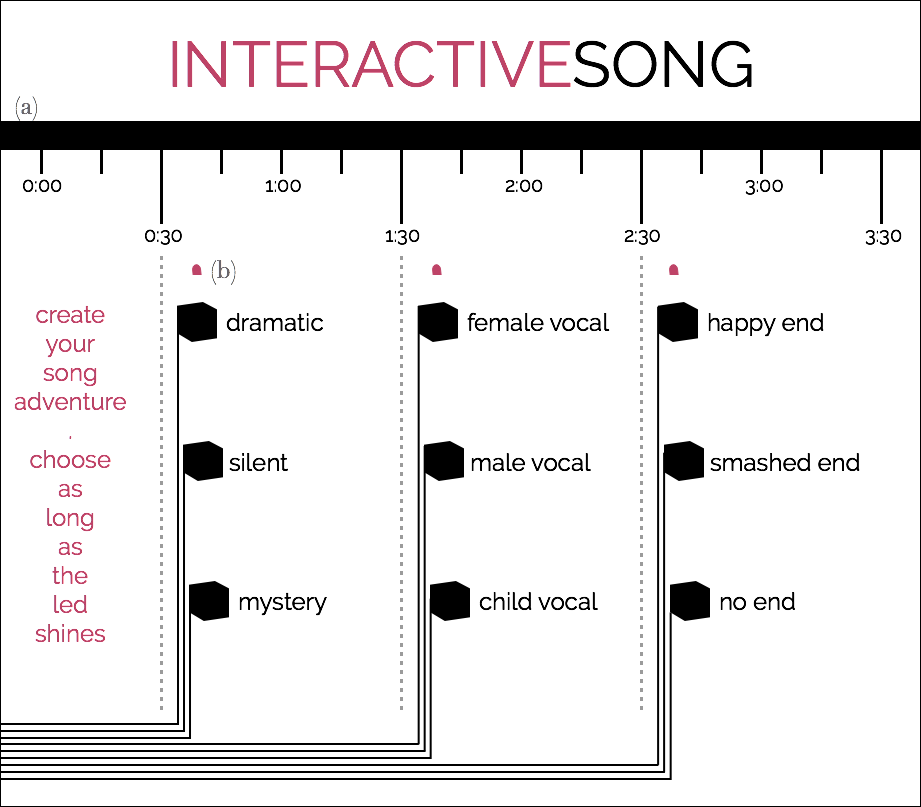
\includegraphics[width=1.0\textwidth]{grafiken/function_interactivesong.png}
\caption{Beispiel-Skizze Interaktiver Song im digitalen Klangbuch}
\label{fig:abb1}
\end{figure}


\textbf{Unterschied zum herkömmlichen Album}\\
Interaktive Songs sind nicht neu. Auf einem Album kann diese Idee jedoch nicht verwirklicht werden. Im Internet gibt es Beispiele zu interaktiven Songs z. B. auf dem Videoportal YouTube\footnote{Interaktiver Song auf YouTube: \url{https://www.youtube.com/watch?v=OtcpO4vipNU}} und dem Storytelling Tool interlude\footnote{interlude:\url{http://blog.interlude.fm/}}.\\


\textbf{Weiteres Nutzungsszenario}
\begin{itemize}
\item Ideenbeispiel 1: Der Interaktive Song kann auf mehrere Seiten im Buch ausgeweitet werden. So kann der Inhalt der Seiten auf jeden "Handlungsstrang" angepasst werden.
\item Ideenbeispiel 2: Der Song kann eine Geschichte erzählen, sowohl grafisch, als auch über den Songtext. Je nach gewählten Handlungsstrang, kann die Geschichte eine andere Wendung nehmen, der Songtext ändert sich. Die verschiedenen Songtexte können im Klangbuch abgebildet und vom Hörer mitgelesen werden.
\end{itemize}



%%%%%%%%%%%%


\subsection{Entstehungsgeschichte Song - "Versions"}
Die Entstehungsgeschichte eines Songs, im Folgenden auch "Versions" genannt, kann im digitalen Klangbuch nicht nur durch Texte und passende Bilder erzählt werden. Der Hörer kann auch in die verschiedenen Versionen, die ein Song von der Idee hin zu einer Live-Version durchläuft, hinein hören. Beispielstationen bei der Entwicklung eines Songs sind folgende:

\begin{itemize}
\item Skizze: Die erste Idee, die auf einem Klavier oder einer Gitarre entsteht
\item Proberaumversion: Die weiter verarbeitete Idee, die mit der Band im Proberaum verfeinert wird
\item Studioversion: Der Song wird professionell in einem Studio aufgenommen
\item Live-Version: Eine Aufnahme, die auf einem Live-Konzert mitgeschnitten wurde
\end{itemize}  


\textbf{Unterschied zum herkömmlichen Album}\\
Der Hörer kennt oftmals nur die Studio- oder Live-Version eines Songs. Der Entstehungsprozess bleibt dabei meist außen vor.\\


%%%%%%%%%%%%%%%%%%%%%%%%%%%%%%%%%%%%%%%%%%%%%%%%%%%%%%%%%%%%%%%%%%%%%%%%%%%%%%%%%%%%%%%%%%%%%%%%
%%%%%%%%%%%%%%%%%%%%%%%%%%%%%%%%%%%%%%%%%%%%%%%%%%%%%%%%%%%%%%%%%%%%%%%%%%%%%%%%%%%%%%%%%%%%%%%%
%%%%%%%%%%%%%%%%%%%%%%%%%%%%%%%%%%%%%%%%%%%%%%%%%%%%%%%%%%%%%%%%%%%%%%%%%%%%%%%%%%%%%%%%%%%%%%%%
%%%%%%%%%%%%%%%%%%%%%%%%%%%%%%%%%%%%%%%%%%%%%%%%%%%%%%%%%%%%%%%%%%%%%%%%%%%%%%%%%%%%%%%%%%%%%%%%
%%%%%%%%%%%%%%%%%%%%%%%%%%%%%%%%%%%%%%%%%%%%%%%%%%%%%%%%%%%%%%%%%%%%%%%%%%%%%%%%%%%%%%%%%%%%%%%%


\chapter{Leitfäden: Arten und Auswahl eines Leitfadens}

Ziel ist es einen Leitfaden zu entwickeln, der die Funktionen und Möglichkeiten des digitalen Klangbuchs erläutert und veranschaulicht. Dem KlangKünstler sollen die Möglichkeiten und der multisensuale Charakter des digitalen Klangbuchs verdeutlicht und Nahe gebracht werden.\\

Im Folgenden werden mögliche Arten von Leitfäden vorgestellt. In einer Bewertungstabelle werden diese anhand von Kriterien gegenüber gestellt und ausgewertet. Anschließend wird ein Leitfaden erstellt.

%%%%%%%%%%%%
%%%%%%%%%%%%
\section{Arten von Leitfäden}



%%%%%%%%%%%%

\subsection{Leitfaden als gedrucktes Handbuch}
Ein gedrucktes Handbuch enthält die Funktionen eines Produkts und beschreibt diese ausführlich. Es dient als Dokumentation, Nachschlagewerk und Anleitung, in dem Bilder und Texte platziert werden können.\\

\textbf{Vorteile}\\
Das Handbuch ist ein gängiges Format zur detaillierten Beschreibung von Funktionen. Der Leitfaden in Form eines gedruckten Handbuchs ließe sich in der Bachelorarbeit realisieren.\\

\textbf{Nachteile}\\
Der Nachteil eines Handbuches ist, dass der KlangKünstler die Funktionsmöglichkeiten nicht aktiv erleben kann: es fehlen Klangbeispiele und Interaktionen, die das Klangbuch ausmachen. Ein gedrucktes Handbuch bietet keine interaktive Suche an. Es ermöglicht nur eine eine Suche über einen abgedruckten Wortindex. Ein gedrucktes Handbuch verliert sehr schnell an seiner Aktualität, sobald eine neue Funktion für das digitale Klangbuch entwickelt wird. Die Distribution für ein gedrucktes Handbuch gestaltet sich schwierig und kostenintensiv.

%%%%%%%%%%%%

\subsection{Leitfaden als digitales Handbuch}
Ein digitalisiertes Handbuch enthält die Funktionen eines Produkts und beschreibt diese ausführlich. Es dient als Dokumentation, Nachschlagewerk und Anleitung, in dem Bilder und Texte platziert werden können. Es kann im gängigen Datei-Format PDF erstellt und bereit gestellt werden.\\


\textbf{Vorteile}\\
Das Handbuch ist ein gängiges Format zur detaillierten Beschreibung von Funktionen. In digitalisierter Form kann es als PDF-Datei zum Download angeboten oder per E-Mail versandt werden. Dokumente im PDF-Format bieten von Haus aus eine Suchfunktion an, mit der sich das Handbuch nach jedem beliebigen Begriff durchsuchen lässt. Es kann es ohne großen Aufwand um weitere Kapitel / Funktionen ergänzt und Fehler korrigiert werden. Die Änderungen werden an einer Datei vorgenommen, die dann, aktualisiert, zum Download angeboten werden kann. Somit kann der Leitfaden immer auf dem neuesten Stand angeboten werden. Im Gegensatz zu einem gedruckten Handbuch, lassen sich klickbare Links in einem PDF integrieren. Der Kostenaufwand für ein digitales Handbuch ist sehr gering: Es treten keine Kosten für die Herstellung des Produkts an sich auf (z. B. Druck). Das Handbuch kann als Begleitmaterial, zum Beispiel zu einer DVD, dienen. \\Der Leitfaden in Form eines digitalen Handbuch ließe sich in der Bachelorarbeit realisieren.\\

\textbf{Nachteile}\\
Der Nachteil eines Handbuches ist, dass der KlangKünstler die Funktionsmöglichkeiten nicht aktiv erleben kann: Es fehlen Klangbeispiele und Interaktionen, die das Klangbuch ausmachen. 


%%%%%%%%%%%%


\subsection{Leitfaden als Digitales Klangbuch}
Der Leitfaden kann als ein funktionierendes digitales Klangbuch entwickelt werden. Jede mögliche Funktion wird in einem Kapitel dargestellt.\\

\textbf{Vorteile}\\
Der KlangKünstler hält mit dem Leitfaden in Form eines digitalen Klangbuchs bereits das funktionierende, multisensuale Produkt in den Händen. Er kann jede Funktion sofort ausprobieren und aktiv erleben. Der Leitfaden kann als exklusives Anschauungsmaterial dienen (z. B. auf Messen, Ausstellungen, Shops, Plattenläden). Die Funktionen können detailliert beschrieben werden.\\

\textbf{Nachteile}\\
Den Leitfaden in Form eines digitalen Klangbuchs zu entwickeln ist kostenintensiv und aufwändig. Es ist nicht für jeden KlangKünstler sofort verfügbar, da es nicht jedem gesendet werden kann, noch lässt es sich (wie z. B. ein PDF) über einen digitalen Verteiler bereitstellen. Der Leitfaden als fertiges, funktionales digitales Klangbuch lässt sich nicht problemlos aktuell halten.\\Der Leitfaden in Form eines funktionierenden digitalen Klangbuchs ließe sich aufgrund der Komplexität des Klangbuchs, der Kosten und des eingeschränkten Zeitrahmens der Bachelorarbeit nicht realisieren.


%%%%%%%%%%%%


\subsection{Leitfaden als Film}\label{LeitfadenAlsFilm}
Der Leitfaden kann als Informationsfilm umgesetzt werden. Die Funktionen können in Teilfilme unterteilt und darin ausführlich dargestellt und beschrieben werden.\\


\textbf{Vorteile}\\
In einem Film ließen sich die Funktionen des Klangbuchs vorführen. Anders als in einem Handbuch handelt es sich hier nicht um eine statische Darstellung durch Texte und Bilder. Der KlangKünstler kann die Interaktion des Klangbuchs miterleben, in dem er sich die Filmsequenz anschaut. Neue Funktionen lassen sich durch weitere Filmsequenzen hinzufügen. Ein Film kann auf eine Website eingebunden oder auch als Begleitmaterial auf einer DVD gespeichert werden. Ebenso wäre es möglich einen Online Video-Kanal zu erstellen, um die Filmsequenzen gebündelt in einem Kanal anzubieten. Der Leitfaden in Form eines Films oder mehreren Filmsequenzen ließe sich in der Bachelorarbeit realisieren.\\


\textbf{Nachteile}\\
In einem Film ist keine Interaktion durch den KlangKünstler möglich. Ein bereits gedrehter Film lässt sich bei einem Fehler / einer Änderung der Funktion nicht ändern, sondern muss neu gedreht werden.


%%%%%%%%%%%%


\subsection{Leitfaden als Video-Kanal}
Der Leitfaden kann in Form eines Video Kanals erstellt werden. Der Kanal enthält dann Filmsequenzen zu den einzelnen Funktionen.\\

\textbf{Vorteile}\\
Videoportale sind derzeit ein beliebtes Ziel für Internetnutzer. Neben dem plattformübergreifenden Bereitstellen von Videomaterial, lassen sich hierüber auch Videos bewerten und \gls{viral} verbreiten. Das Videoportal YouTube beispielsweise, hat weltweit mehr als 1 Milliarde Nutzer.\cite{YT} Um das digitale Klangbuch und seine Funktionen zu verbreiten, ist ein eigener Videokanal demzufolge hilfreich. Zusätzlich ist es auf YouTube möglich hochgeladene Filme mit klickbaren Links auszustatten. Ein Videoportal bietet ebenfalls die Möglichkeit folgende Daten auszuwerten:
\begin{itemize}
\item Wie oft wurde ein \gls{videoclip} angeschaut?
\item Wie viele positive / negative Bewertungen hat der \gls{videoclip} erhalten?
\item Kommentare von Nutzern
\end{itemize}
Der Leitfaden in Form eines Video-Kanals mit dazugehörenden Filmsequenzen ließe sich in der Bachelorarbeit realisieren.\\

\textbf{Nachteile}\\
Die Nachteile, die unter "Leitfaden als Film"\ref{LeitfadenAlsFilm} definiert sind, gelten auch für einen Video-Kanal.

%%%%%%%%%%%%


\subsection{Leitfaden als Website}
Auf einer Website lassen sich die Funktionen des digitalen Klangbuchs anschaulich darstellen und detailliert beschreiben.\\

\textbf{Vorteile}\label{VorteileWebsite}\\
Der Leitfaden als Website bietet die Möglichkeit Inhalte in Form von Texten, Bildern, Videos, Ton und Animationen darzustellen. Die Website bietet genügend Raum um die Funktionen detailliert und anschaulich darzustellen. Die Seite kann von jedem KlangKünstler über das Internet aufgerufen werden. Neue Funktionen und Änderungen lassen sich einfach und zu jeder Zeit einpflegen. Durch den Einsatz von bestimmten Techniken ließen sich die Funktionen des digitalen Klangbuchs über die Website simulieren. So könnte der Besucher der Website die Funktionen online ausprobieren. Eine Website bietet ebenfalls die Möglichkeit statistische Daten auszuwerten, z. B. wie oft eine Seite besucht oder ein Link angeklickt wurde.\\Der Leitfaden in Form einer Website ließe sich in der Bachelorarbeit realisieren.\\ 

\textbf{Nachteile}\\
Der KlangKünstler hält bei einer Website nichts in den Händen. Die Haptik, die das digitale Klangbuch ausmachen, ist nicht vorhanden.

%%%%%%%%%%%%

\section{Bewertungstabelle Leitfaden}

Die vorgestellten Leitfäden werden anhand der folgenden Tabelle gegenüber gestellt und bewertet. Je höher die Punktzahl, desto geeigneter ist der Leitfaden für das digitale Klangbuch. Die Bewertungsskala pro Kriterium liegt im Bereich von 0 bis 5 Punkten.


\begin{figure}[!ht]
		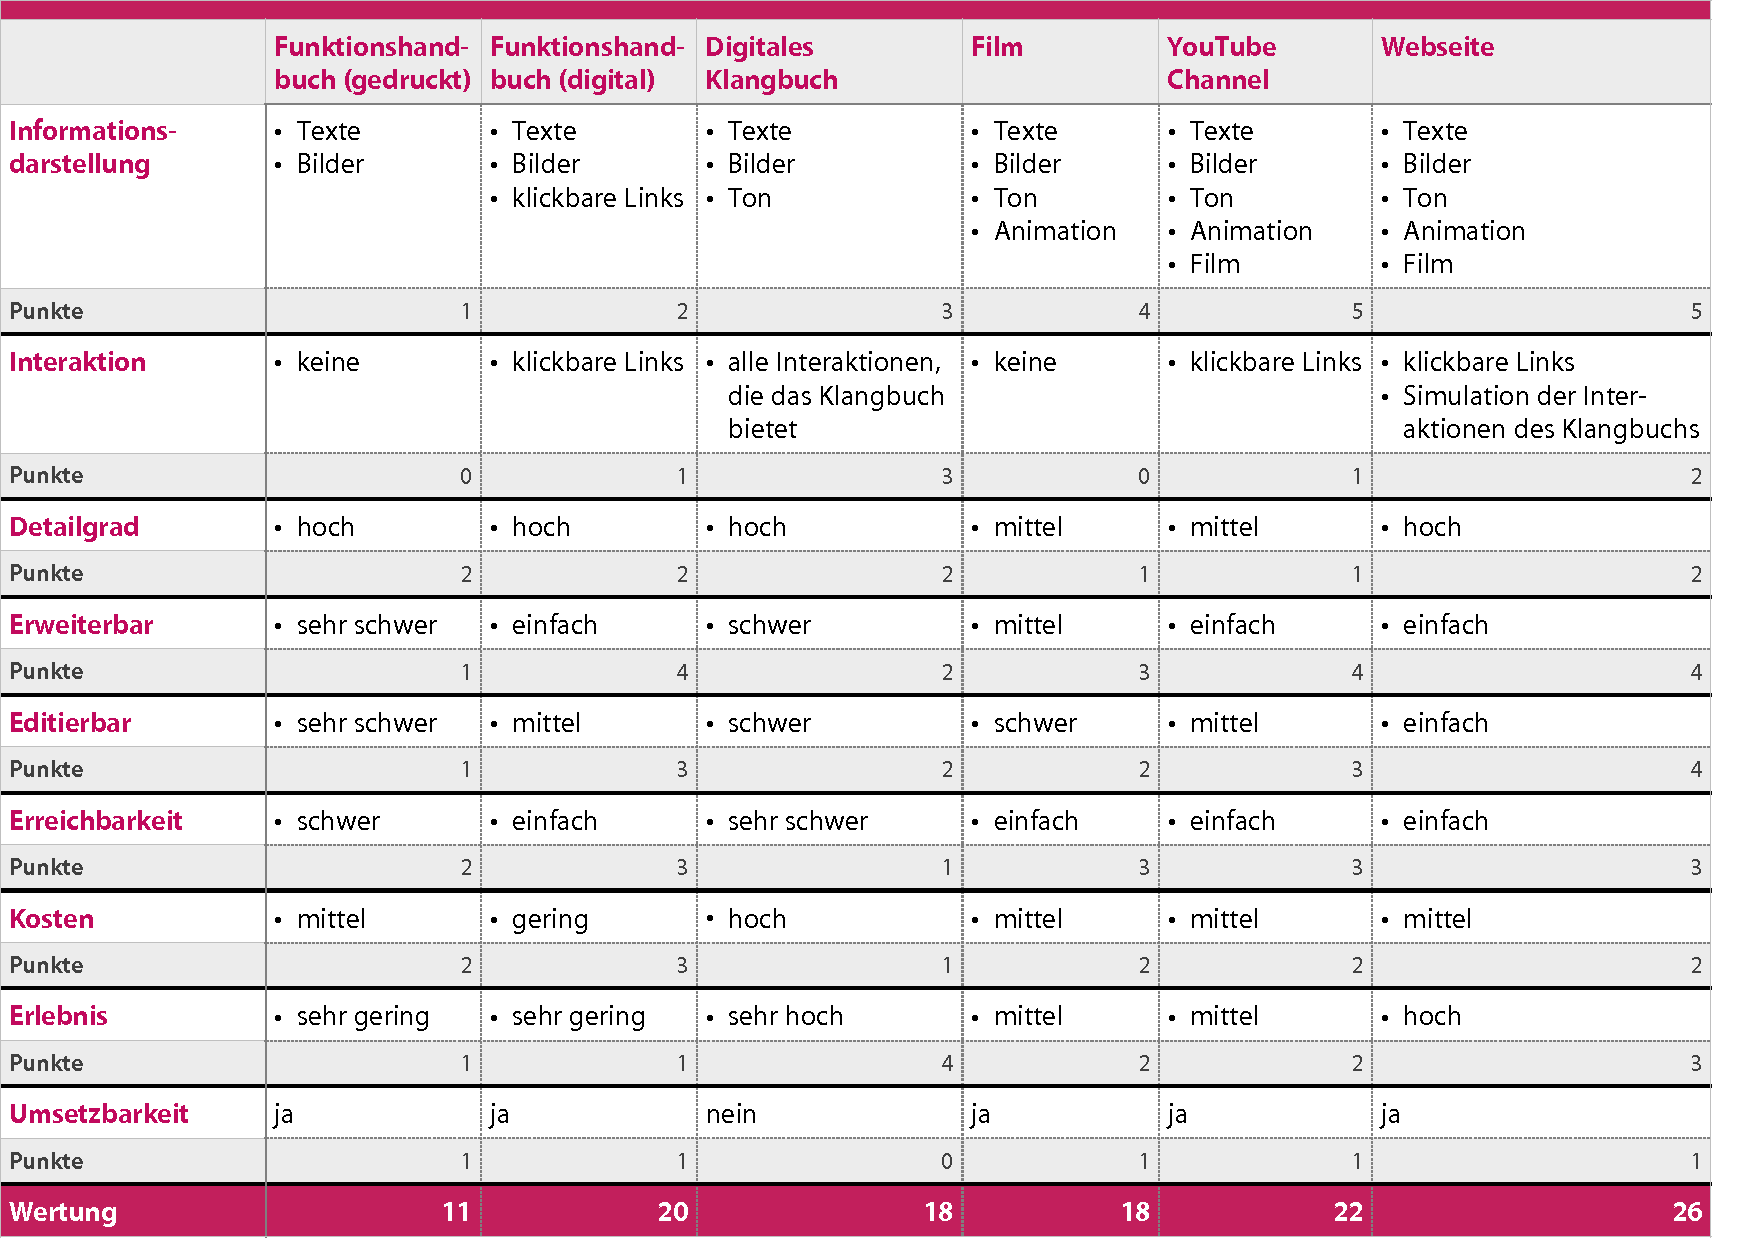
\includegraphics[natwidth=920pt, natheight=95pt, width=1.0\textwidth]{grafiken/leitfaden-bewertung.pdf}
\caption{Bewertungstabelle der möglichen Leitfäden}
\end{figure}


\textbf{Informationsdarstellung}\\
In welcher Form können Informationen zu den Funktionen dargestellt werden?\\
Ein Video-Kanal und eine Website bieten hier alle Möglichkeiten zur Darstellung von Informationen.\\

\textbf{Interaktion}\\
Bietet der Leitfaden dem KlangKünstler eine realistische Interaktion?\\
Der Leitfaden als digitales Klangbuch ist die realste Möglichkeit die Funktionen des digitalen Klangbuchs darzustellen. Dem KlangKünstler werden alle Interaktionen geboten.\\

\textbf{Detailierungsgrad}\\
Wie detailliert lassen sich die Funktionen und Informationen zum digitalen Klangbuch darstellen?\\
Informationen, die zu einer Filmsequenz auf einem Video-Kanal hinterlegt werden können, sind begrenzt.\\


\textbf{Erweiterbarkeit}\\
Lässt sich der Leitfaden problemlos erweitern?\\
Ein digitales Funktionshandbuch, eine Video-Kanal und eine Website lassen sich problemlos erweitern. Ein fertiger Film und ein gedruckter Leitfaden dagegen nicht.\\


\textbf{Editierbarkeit}\\
Lassen sich Informationen im Leitfaden problemlos ändern?\\
Ein digitales Funktionshandbuch, eine Website und die Informationen in einem Video-Kanal lassen sich problemlos ändern. Ein fertiger Film und ein gedruckter Leitfaden dagegen nicht.\\


\textbf{Erreichbarkeit}\\
Ist der Leitfaden für jeden KlangKünstler frei verfügbar / erreichbar?\\
Eine Website und ein Video-Kanal ist für jeden KlangKünstler frei verfügbar. Ein gedruckter Leitfaden muss erst seinen physischen Weg zum KlangKünstler finden.\\


\textbf{Aktualität}\\
Die Aktualität ist nicht in der Tabelle enthalten. Sie bildet sich aus den Kriterien Erweiterbarkeit, Editierbarkeit und Erreichbarkeit. Der Leitfaden ist nur dann so aktuell, wie er auch verändert, ergänzt und erreicht / verteilt werden kann.\\Ein Leitfaden als eigenes Objekt, wie z. B. ein digitales Handbuch (PDF-Datei) oder eine Filmsequenz verlieren ihre Aktualität sobald eine neue Version davon erstellt wurde. Die Anlaufstelle für den KlangKünstler dagegen - in diesem Fall eine Website oder ein Video-Kanal - kann immer den aktuellsten Leitfaden zur Verfügung stellen.\\
Zählt man die vergebenen Punkte der einzelnen Leitfäden für die Kriterien Erweiterbarkeit, Editierbarkeit und Erreichbarkeit zusammen ergibt sich daraus die Bewertung der Aktualität.\\

\textbf{Kosten}\\
Wie hoch sind die Kosten zur Umsetzung des Leitfadens?\\
Die Funktionen müssen für jeden Leitfaden erstellt und beschrieben werden. Ein Handbuch muss jedoch für jeden KlangKünstler gedruckt und versendet werden. Ein digitales Klangbuch als Leitfaden enthält neben Papier auch Technik und die Produktionskosten, die für die Herstellung eines digitalen Klangbuchs notwendig sind. Die Kosten für das Hosting einer Website und das Drehen von Filmsequenzen sind dagegen deutlich geringer.\\

\textbf{Erlebnis}\\
Vermittelt der Leitfaden dem KlangKünstler das besondere Erlebnis des digitalen Klangbuchs?
Nur das Klangbuch selbst kann dem KlangKünstler einen realen Einblick und ein reales Erleben ermöglichen. Durch Webtechnologien ist es möglich die Funktionen des digitalen Klangbuchs auch auf einer Website zu simulieren. In Filmsequenzen lassen sich die Funktionen des digitalen Klangbuchs durch ein Abfilmen des Klangbuchs vermitteln.\\

\textbf{Umsetzbarkeit}\\
Lässt sich der vorgestellte Leitfaden im Rahmen der Bachelorarbeit umsetzen?\\
Das digitale Klangbuch als Leitfaden ist aufgrund der eingesetzten Technik und den damit verbunden Kosten im Rahmen der Bachelorarbeit zu komplex um es zu realisieren. Alle anderen vorgestellten Leitfäden sind umsetzbar.\\


%%%%%%%%%%%%

\subsection{Auswahl Leitfaden}
Die höchste Punktzahl hat der Leitfaden als Website erhalten. Die Vorteile einer Website wurden bereits in "Leitfaden als Website" in Kapitel \ref{VorteileWebsite} genannt. Eine Website bietet den Vorteil, dass sie immer aktuell gehalten und erweitert werden kann. Durch Kombination aus Film, Text und Bildern lässt sich der Leitfaden nicht nur detailliert sondern auch anschaulich darstellen. Der KlangKünstler kann durch das Schauen der Filmsequenzen eine ungefähre Idee des digitalen Klangbuchs erhalten und die Funktionen "miterleben".\\
Im weiteren Verlauf der Arbeit werden die Begriffe "Leitfaden" und "Website" synonym verwendet.\\



%%%%%%%%%%%%%%%%%%%%%%%%%%%%%%%%%%%%%%%%%%%%%%%%%%%%%%%%%%%%%%%%%%%%%%%%%%%%%%%%%%%%%%%%%%%%%%%%
%%%%%%%%%%%%%%%%%%%%%%%%%%%%%%%%%%%%%%%%%%%%%%%%%%%%%%%%%%%%%%%%%%%%%%%%%%%%%%%%%%%%%%%%%%%%%%%%
%%%%%%%%%%%%%%%%%%%%%%%%%%%%%%%%%%%%%%%%%%%%%%%%%%%%%%%%%%%%%%%%%%%%%%%%%%%%%%%%%%%%%%%%%%%%%%%%
%%%%%%%%%%%%%%%%%%%%%%%%%%%%%%%%%%%%%%%%%%%%%%%%%%%%%%%%%%%%%%%%%%%%%%%%%%%%%%%%%%%%%%%%%%%%%%%%
%%%%%%%%%%%%%%%%%%%%%%%%%%%%%%%%%%%%%%%%%%%%%%%%%%%%%%%%%%%%%%%%%%%%%%%%%%%%%%%%%%%%%%%%%%%%%%%%







\chapter{Konzeption Leitfaden}

Im ersten Schritt dieses Kapitels werden die Ziele des Leitfadens definiert. Anschließend wird definiert, wie der Leitfaden idealerweise aufgebaut werden sollte. Im letzten Schritt werden die \gls{videoclip}s konzipiert und Drehbücher dazu erstellt.


%%%%%%%%%%%%
%%%%%%%%%%%%
%%%%%%%%%%%%


\section{Art des Leitfaden}
Der Leitfaden wird als Webseite konzipiert und umgesetzt. Dazu werden Videoclips erstellt und in die Webseite eingebunden. Durch die Kombination aus Videoclips, Text und Bildern lässt sich der Leitfaden nicht nur detailliert sondern auch anschaulich darstellen. 

%%%%%%%%%%%%
%%%%%%%%%%%%
%%%%%%%%%%%%


\section{Vermittlungsziele Leitfaden}
Was soll der Leitfaden vermitteln?

\begin{itemize}
\item Der KlangKünstler soll das Gesamtkonzept "Digitales Klangbuch" verstehen
\item Der KlangKünstler soll den Aufbau des digitalen Klangbuchs verstehen
\item Dem KlangKünstler sollen die Möglichkeiten und Grenzen des digitalen Klangbuchs vermittelt werden
\item Der KlangKünstler soll mögliche Funktionen des digitalen Klangbuchs kennen und verstehen lernen
\item Bei den Besuchern der Website soll Interesse und Begeisterung für das digitale Klangbuch geweckt werden
\item Der KlangKünstler soll inspiriert werden
\end{itemize}


%%%%%%%%%%%%
%%%%%%%%%%%%
%%%%%%%%%%%%

\section{Aufbau Leitfaden}


%%%%%%%%%%%%


\subsection{Einstieg}
Damit der Besucher der Website das digitale Klangbuch kennen und verstehen lernt, soll das digitale Klangbuch erklärt und folgende Fragen beantwortet werden:

\begin{itemize}
\item Was ist das digitale Klangbuch?
\item Was kann man mit dem digitalen Klangbuch machen?
\item Was ist das Besondere an dem digitalen Klangbuch?
\item An wen richtet sich das digitale Klangbuch?
\end{itemize}

Ein kurzes Einführungsvideo, in dem das digitale Klangbuch vorgestellt wird, kann all diese Fragen beantworten. Dieser \gls{videoclip} wird im Folgenden "Startclip" genannt.


%%%%%%%%%%%%


\subsection{Kategorien}
Das digitale Klangbuch bedient mehrere Sinne: den auditiven, visuellen und haptischen Sinn. Da in den Funktionen des Klangbuchs zumeist alle drei Sinne gleichzeitig angesprochen werden, ist eine Unterteilung der Funktionen in die Bereiche Audio, Visuell und Haptik nicht sinnvoll. Jedoch kann im Leitfaden zu jedem dieser Sinne ein Erklärungstext mit Beispielen integriert werden.\\


%%%%%%%%%%%%


\subsection{Auswahl der Klangbuch-Funktionen}
Aufgrund des zeitlich eingeschränkten Rahmens der Bachelorarbeit ist es nicht möglich jede Funktion in einem Video vorzustellen, denn jeder \gls{videoclip} benötigt passendes Audiomaterial, das produziert werden muss. Die Auswahl der Funktionen erfolgte nach folgenden Kriterien:\\

1. Erlebnis / Besonderheit der Funktion\footnote{Erlebnis / Besonderheit im Sinne von: Die vorzustellende Funktion soll ein besonderes Erleben beim Klangkünstler und Hörer hervor rufen und die besonderen Möglichkeiten des digitalen Klangbuchs aufweisen.}\\ 
2. Mindestens eine komplexere Funktion soll umgesetzt werden (z. B. Multitrack)\\
2. Produzierbarkeit des passendes Audiomaterials im Rahmen der Bachelorarbeit\\

Folgende Funktionen wurden ausgewählt:

\begin{itemize}
\item Audio abspielen (Standardfunktion)
\item Multitrack 
\item SongKit
\item Entstehungsgeschichte \gls{song}, im Folgenden "Versions" genannt
\end{itemize}

Weitere Funktionen werden ohne \gls{videoclip} auf der Website vorgestellt. Die haptischen und visuellen Funktionen werden im Einführungsclip vorgestellt.


%%%%%%%%%%%%%%%%%%%%%%%%%%%%%%%%%%%%%%%%%%%%%%%%
%%%%%%%%%%%%%%%%%%%%%%%%%%%%%%%%%%%%%%%%%%%%%%%%
%%%%%%%%%%%%%%%%%%%%%%%%%%%%%%%%%%%%%%%%%%%%%%%%


\section{Konzeption Videoclips}

Für jeden \gls{videoclip} muss ein \gls{song} oder Soundfragment produziert, ein Layout entwickelt und ein Drehbuch inklusive Storyboard erstellt werden. Nach Aufnahme der \gls{videoclip}s werden diese am Rechner montiert und vertont.

\subsection{Produktion Songs / Sounds}
Um die entwickelten, akustischen Funktionsmöglichkeiten in \gls{videoclip}s zu veranschaulichen, wurden passende lizenzfreie \gls{song}s und Soundfragmente benötigt. Diese wurde zum Teil selbst produziert.


\begin{figure}[H]
\centering
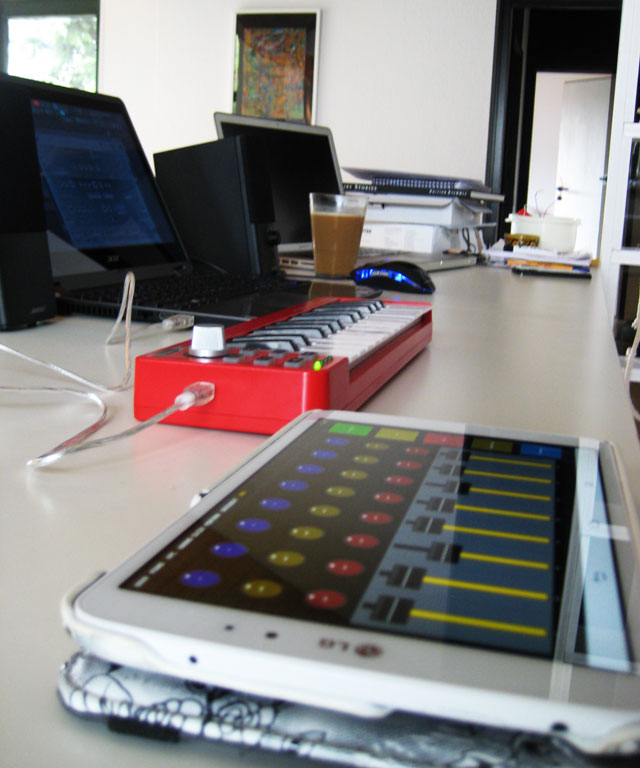
\includegraphics[width=0.5\textwidth]{grafiken/musikproduktion.jpg}
\caption{Produktion der Songs und Soundfragmente}
\end{figure}

Für den \textbf{Start-\gls{clip}} wurde ein \gls{loop} aus der Sound-Bibliothek der Musikproduktions-Software Garageband von Apple ausgewählt und Stimmaufnahmen produziert.\\

Ein \gls{song} mit sieben einzelnen Spuren wurde für den \gls{clip} \textbf{Multitrack} produziert.\\

Für den \gls{clip} \textbf{SongKit} wurden 13 zueinander passende \gls{loop}s produziert. Diese unterteilen sich in Bass, Drums, Melodie, Pad und Effekt.\\

Ein \gls{song} in fünf Versionen wurde für den \gls{clip} \textbf{Versions} produziert: Skizze-, Probe-\\raum-, Studio-, Akustik- und Live-Version. 


%%%%%%%%%%%%
%%%%%%%%%%%%


\subsection{Design \& Layouts}\label{design}
Für den Leitfaden wurde ein Design entwickelt, welches Schriften, Farben und das Logo beinhaltet. Anhand dieser Vorgaben wurden die Layouts für die ausgewählten Funktionen entwickelt. Die Grafiken in den Layouts wurden größtenteils selbst erstellt, einige stammen von der lizenzfreien Bildbörse Pixabay\footnote{Lizenzfreie Bildbörse Pixabay, die verwendeten Bilder benötigen keinen Bildnachweis: \url{https://pixabay.com}}.

\begin{figure}[H]
\centering
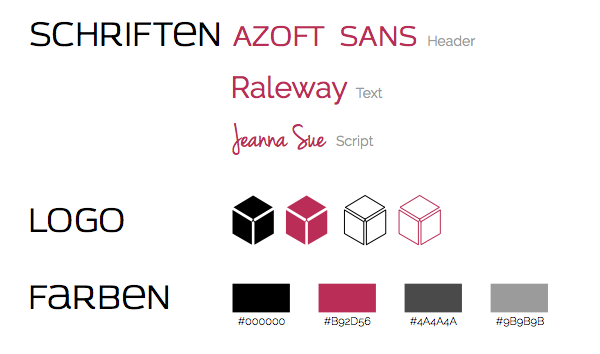
\includegraphics[width=0.7\textwidth]{grafiken/corporatedesign1.png}
\caption{Design: Schriften, Farben und Logo}
\label{fig:design}
\end{figure}

\subsubsection{Logo}
Bei der Entwicklung des Logos wurden wichtige und interessante Merkmale des digitalen Klangbuchs ermittelt:
\begin{itemize}
\item drei Sinne: Hör-, Seh-, Tastsinn
\item alle Sinne werden zugleich angesprochen
\item berührungsempfindliche Elemente
\item das Buch enthält technische Komponenten
\item Erlebnis
\end{itemize}

Anhand der Merkmale wurde ein Logo entwickelt; nicht jedes Merkmal konnte in dem Logo wieder gespiegelt werden:\\
Die drei Sinne können durch drei Teile symbolisiert werden. Da alle Sinne gleichzeitig angesprochen werden, sollten alle Teile miteinander verbunden werden. Das Logo kann so gestaltet werden, dass es an einen \gls{button} erinnert. So kann die Berührungsempfindlichkeit des Buches im Logo dargestellt werden. Klare Linien unterstreichen die technische Ausrichtung des Buches.

\begin{figure}[H]
\centering

\includegraphics[width=0.7\textwidth]{grafiken/logo.png}
\caption{Design: Schriften, Farben und Logo}
\label{fig:logo}
\end{figure}

Das entwickelte Logo kann in den Farben (s. Farbwerte in Abbildung \ref{fig:design}) Pink oder Schwarz dargestellt werden. Es kann zudem gefüllt oder nur aus Außenlinien bestehen.\\
Das Logo dient in den Layouts grundsätzlich als \gls{button} um eine Audiodatei zu starten oder zu stoppen.

%%%%%%%%%%%%
%%%%%%%%%%%%


\subsection{Digitales Klangbuch}

Die \gls{videoclip}s sollen dem KlangKünstler das digitale Klangbuch näher bringen. Dazu ist es sinnvoll das digitale Klangbuch in den Videos zu präsentieren. Dazu wurde ein nichtfunktionaler Prototyp erstellt.\\

\begin{figure}[H]
\centering

\includegraphics[width=0.8\textwidth]{grafiken/cutting.png}
\caption{Die gedruckten Layouts wurden mit einem Cutter-Messer ausgeschnitten und in ein Buch geklebt}
\end{figure}


Ein großformatiges Buch dient dazu als Basis. Für jeden \gls{videoclip} wurde ein Layout entwickelt, gedruckt und in das Buch montiert. Ein Audioeingang für den Kopfhörer wurde ebenfalls in das Buch integriert.\\


\begin{figure}[H]
\centering
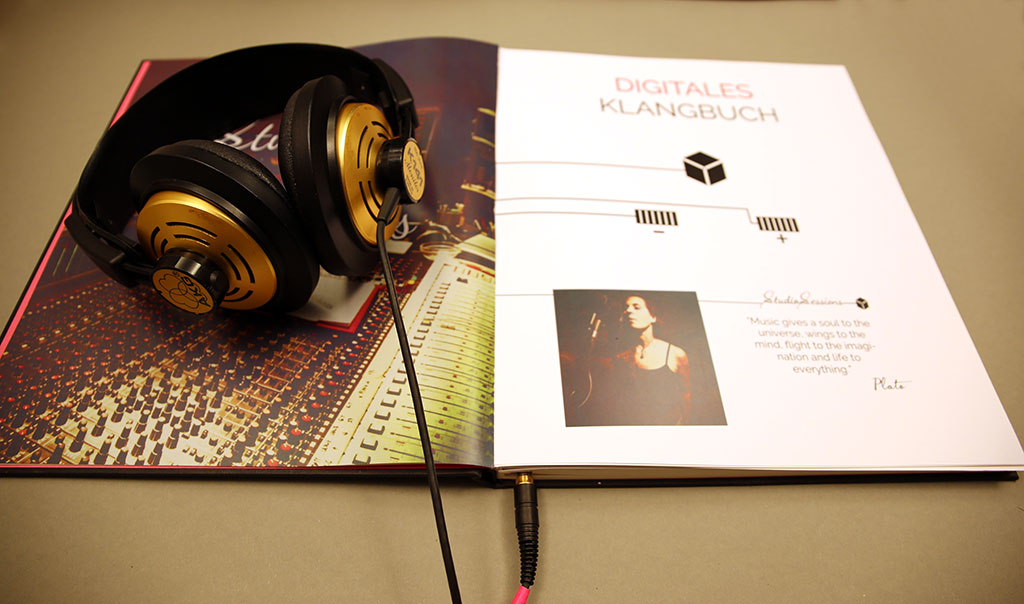
\includegraphics[width=0.9\textwidth]{grafiken/gebautes_klangbuch.jpg}
\caption{Prototyp des digitalen Klangbuchs}
\end{figure}

%%%%%%%%%%%%
%%%%%%%%%%%%




\subsection{Konzeption Intro \& Outro}
Jeder \gls{videoclip} wird ähnliche aufgebaut. Der Vorteil daran ist, dass die Videoclips so einen Wiedererkennungseffekt und ein konsistentes, professionelles Erscheinungsbild haben.\\


\textbf{\gls{intro}}\\
Der Name des Videoclips oder der Funktion, die in dem Videoclip vorgestellt wird, soll eingeblendet werden.
Darunter das Logo des Digitalen Klangbuchs. Folgendes Material wird benötigt:

\begin{itemize}
\item digitales Klangbuch
\item Kopfhöreranschluss
\item Kopfhörer
\item evtl. \gls{loop}
\end{itemize}

\vspace{0.5cm}

Folgendes \gls{intro}-Layout wurde entwickelt:

\begin{figure}[H]
\centering

\includegraphics[width=1.0\textwidth]{grafiken/layoutintro.png}
\caption{Layout des \gls{intro}s für die Funktion Multitrack}
\end{figure}


\textbf{\gls{outro}}\\
Der Schriftzug "Digitales Klangbuch" mit dem Logo, ein Hinweis auf die Website und die Urheberrechte sollen integriert werden.\\

Folgendes \gls{outro}-Layout wurde entwickelt:

\begin{figure}[H]
\centering
\frame{
\includegraphics[width=0.8\textwidth]{grafiken/layoutoutro.png}}
\caption{Layout des \gls{outro}s}
\end{figure}


%%%%%%%%%%%%
%%%%%%%%%%%%

\subsection{Konzeption "Startclip"}
Der Startclip wird als Einführungsvideo auf der Startseite der Website eingebunden. Dem Besucher der Seite soll damit das Buch im Allgemeinen erklärt werden. Dazu wird ein \gls{button} zum Starten und Stoppen des Klangs, eine Lautstärkeregelung und Bilder und Texte integriert. Da der Startclip keine einzelne Funktion vorführt, sondern das Buch an sich präsentiert, wird hier nicht das zuvor entwickelte \gls{intro}, sondern ein eigenes integriert. Dieses hat den folgenden Ablauf:

\begin{itemize}
\item Aufnahme des geschlossenen Buches mit beiliegenden Kopfhörern
\item Kopfhörer werden aufgesetzt
\item der Kopfhörer wird an das Buch angeschlossen
\item das Buch wird aufgeblättert
\end{itemize}


\textbf{Material für den Videoclip}
\begin{itemize}
\item Klangbuch
\item Kopfhörer
\item doppelseitiges Layout mit Bildern, Texten, Lautstärkeregelung, Start\gls{button}
\item Song I (ca. 20 Sekunden)
\item 2. Layout nach Umblättern (z. B. Layout von Multitrack)
\item Song II (ca. 10 Sekunden) (z. B. Song von Multitrack)
\end{itemize}

\vspace{0.5cm}



\textbf{Layout "Startclip"}\\
Das doppelseitige Layout enthält Bilder, Texte und Interaktionsschaltflächen. Die linke Seite zeigt ein Druckbeispiel für ein Foto und einen Titel. Auf der rechten Seite gibt es eine Schaltfläche zum Starten und Stoppen des \gls{song}s und \gls{button}s zur Regelung der Lautstärke. Es ist ebenfalls ein Foto und ein Text abgedruckt. Dazu gibt es einen weiteren \gls{button}, der mit einer Überschrift verbunden ist "Studio Sessions".Jedes berührungsempfindliche Element ist mit einer schwarzen Linie mit dem Buchrücken verbunden. Die Linien berühren sich nicht. Die Linien wurden bewusst so platziert, dass sie kaum versehentlich berührt werden können.


\begin{figure}[H]
\centering
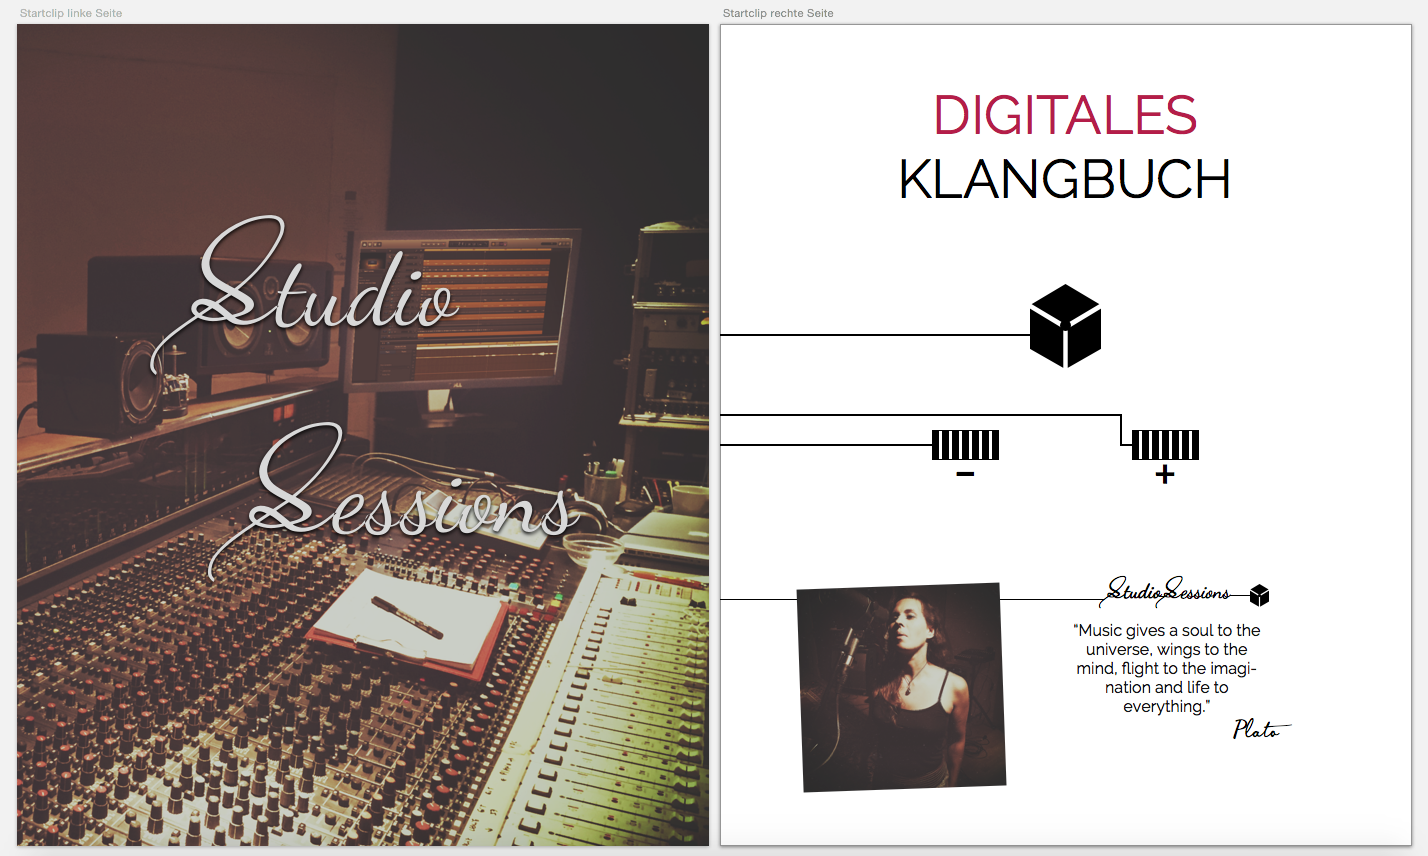
\includegraphics[width=1.0\textwidth]{grafiken/startclip.png}
\caption{Layout für den Startclip. Links: Printbeispiel, Hintergrundfoto mit Titel\\Rechts: Interaktionsmöglichkeiten: Start-/Stopp \gls{button} für den \gls{song}, Lautstärkeregelung, Start-/Stopbutton zum Text}
\label{fig:startclip}
\end{figure}


\vspace{0.5cm}





%%%%%%%%%%%%
%%%%%%%%%%%%
%%%%%%%%%%%%



\subsection{Konzeption "Multitrack"}
Für die Funktion Multitrack wurde der \gls{song} "Sunday Sessions" mit 7 einzelnen Spuren produziert. Im Video soll die Mehrspur-Funktion veranschaulicht werden, in dem einzelne Spuren stumm und wieder angeschaltet werden. Auch die Lautstärke soll sich regeln lassen.\\

Das Layout für die Funktion Multitrack soll auf das Wesentliche, die berührungsempfindlichen Elemente, reduziert sein. Hier liegt der Fokus auf die Interaktionsmöglichkeiten, die die Funktion bietet. Um die aktivierten Spuren kenntlich zu machen, bietet es sich an, diese mit SMD-LEDs zu versehen. Da das digitale Klangbuch ein nichtfunktionaler Prototyp ist, müsste das Leuchten der SMD-LEDs in der Filmmontage simuliert werden. Aus zeitlichen Gründen wurde die Idee der integrierten SMD-LEDs verworfen.\\

Ziel des Clips ist es dem KlangKünstler die Möglichkeit zur Einbindung einer interaktiven Mehrspur-Funktion zu vermitteln.\\


\textbf{Material für den Videoclip}
\begin{itemize}
\item Klangbuch
\item Kopfhörer
\item Layout mit 7 Spuren, Lautstärkeregelung, Startbutton, \gls{button} um alle Spuren aus zustellen.
\item Song mit 7 Spuren
\item Story
\end{itemize}

\vspace{0.5cm}



\textbf{Layout "Multitrack"}\\
Das Layout ist auf das Wesentliche, die berührungsempfindlichen Elemente, reduziert. Es gibt eine Schaltfläche zum Starten und Stoppen des \gls{song}s (\gls{button} neben "Sunday Sessions") und eine zum Stummschalten aller Spuren (\gls{button} neben "Off All"). Die Spuren sind breit gestaltet und beschriftet. Neben jeder Spur befinden Elemente zur Lautstärkeregelung. Jedes berührungsempfindliche Element ist mit einer schwarzen Linie mit dem Buchrücken verbunden. Die Linien berühren sich nicht. Die Linien wurden bewusst so platziert, dass sie kaum versehentlich berührt werden können.

\begin{figure}[H]
\centering
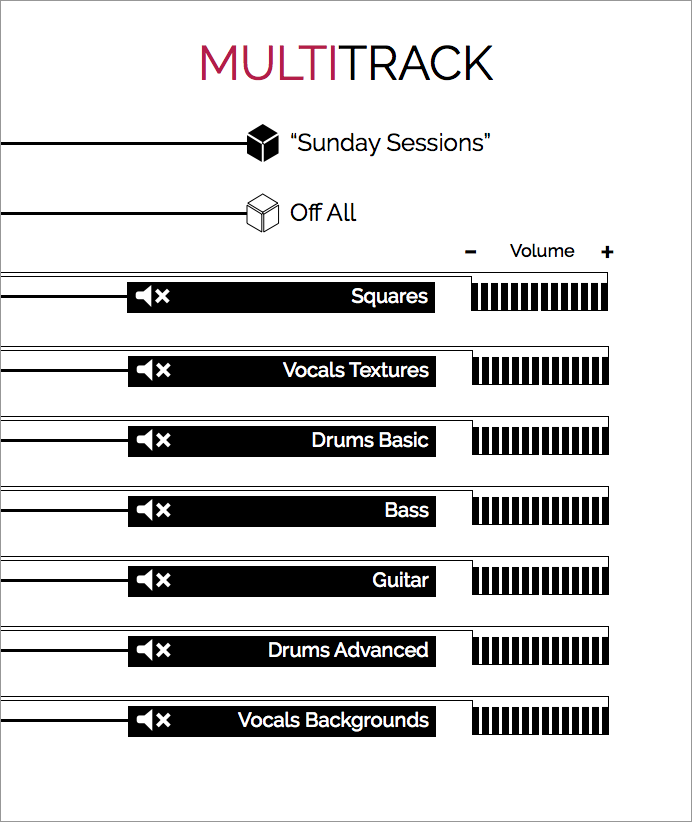
\includegraphics[width=0.6\textwidth]{grafiken/multitrack.png}
\caption{Layout für die Funktion Multitrack.}
\end{figure}

\vspace{0.5cm}




%%%%%%%%%%%%


\subsection{Konzeption "SongKit"}
Für die Funktion SongKit wurde der \gls{loop} "Monday Sessions" mit fünf Spuren und jeweils fünf Variationen erstellt. Im Video soll der Nutzer den \gls{loop} verändern, in dem er auf die verschiedenen Variationen der fünf Spuren klickt.\\

Das Layout für die Funktion SongKit soll auf das Wesentliche, die berührungsempfindlichen Elemente, reduziert sein. Hier liegt der Fokus auf die Interaktionsmöglichkeiten, die die Funktion bietet. Um die Spuren voneinander zu unterscheiden zu können, soll jede Spur mit eigenen Symbolen ausgestattet werden. Um die aktivierten \gls{loop}s kenntlich zu machen, bietet es sich an die Spuren mit SMD-LEDs zu versehen. Da das digitale Klangbuch ein nichtfunktionaler Prototyp ist, müsste das Leuchten der SMD-LEDs in der Filmmontage simuliert werden. Aus zeitlichen Gründen wurde die Idee der integrierten SMD-LEDs jedoch verworfen.\\

Ziel des Clips ist es dem KlangKünstler die Funktion SongKit zu vermitteln und ihn zu neuen Ideen zu inspirieren. Die Funktion SongKit eignet sich z. B. dafür, um unveröffentlichtes, unvollendetes Material dem Fan zur Verfügung zu stellen.\\


\textbf{Material für den Videoclip}
\begin{itemize}
\item Klangbuch
\item Kopfhörer
\item Layout mit fünf Spuren zu je fünf Variationen + Startbutton
\item \gls{loop} mit fünf Spuren zu mind. drei Variationen (es müssen nicht alle Variationen im Videoclip angesteuert werden)
\item Story
\end{itemize}

\vspace{0.5cm}



\textbf{Layout "SongKit"}\\
Das Layout ist auf das Wesentliche, die berührungsempfindlichen Elemente, reduziert. Es gibt eine Schaltfläche zum Starten und Stoppen des \gls{song}s (\gls{button} neben "Monday Sessions"). Jede Spur enthält fünf \gls{loop}s, die mit einem Symbol dargestellt werden. Jede Spur hat dabei ein eigenes Symbol. Jedes berührungsempfindliche Element ist mit einer schwarzen Linie mit dem Buchrücken verbunden. Die Linien berühren sich nicht. Die Linien wurden bewusst so platziert, dass sie kaum versehentlich berührt werden können.

\begin{figure}[H]
\centering

\includegraphics[width=0.6\textwidth]{grafiken/songkit.png}
\caption{Layout für die Funktion SongKit.}
\end{figure}

\vspace{0.5cm}


%%%%%%%%%%%%


\subsection{Konzeption "Versions"}
Für die Funktion Versions wurde der \gls{song} "We are here" in vier Versionen produziert: Als Skizze, eine Proberaumversion, eine Studioversion und eine Aufnahme von einem Live-Auftritt. Zusätzlich dazu wurde noch eine Akustik-Version erstellt. Diese vier Versionen (+ Akustik Version), die der \gls{song} durchläuft, sollen im Videoclip vorgestellt werden.\\ 

Das Layout für die Funktion Versions soll vor allem ein Beispiel zu den visuellen Darstellungsmöglichkeiten im Klangbuch sein: Darstellung von Bildern, Informationen, Songtexten, etc.\\

Ziel des Clips ist es dem KlangKünstler zum Einen die Funktion Versions zu vermitteln. Ihm sollen aber auch die Möglichkeiten zur Darstellung von grafischem und textuellen Inhalten Nahe gebracht werden. Er soll dazu inspiriert werden mehr über sich und die Musik zu erzählen. Material, was bisher auf einer Website, in einem \gls{artwork} oder \gls{booklet} platziert wurde oder unveröffentlicht blieb, hat mehr Raum im digitalen Klangbuch.\\


\textbf{Material für den Videoclip}
\begin{itemize}
\item Klangbuch
\item Kopfhörer
\item vier doppelseitige Layouts mit Startbutton + Fotos + Text
\item Song in vier Versionen + Akustik Version
\item Story
\end{itemize}

\vspace{0.5cm}



\textbf{Layout "Versions"}\\
Für die Visualisierung der Funktion Versions wurde zu jeder \gls{song}-Version ein doppelseitiges Layout erstellt. Die linke Seite ist vollflächig mit einem Bild, passend zur vorgestellten \gls{song}-Version, gefüllt. Die Seite ist jeweils mit dem Namen des \gls{song}s "We are here" und der Version des \gls{song}s betitelt, z. B. Proberaum. Die linke Seite enthält je einen \gls{button} zum Starten und Stoppen des \gls{song}s. Der Titel des \gls{song}s und der \gls{song}-Version werden ebenfalls aufgeführt. Die Seiten sind außerdem mit passenden Bildern und Blindtexten gefüllt. Jedes berührungsempfindliche Element ist mit einer schwarzen Linie mit dem Buchrücken verbunden. Die Linien berühren sich nicht. Die Linien wurden bewusst so platziert, dass sie nicht versehentlich berührt werden können.

\begin{figure}[H]
\centering
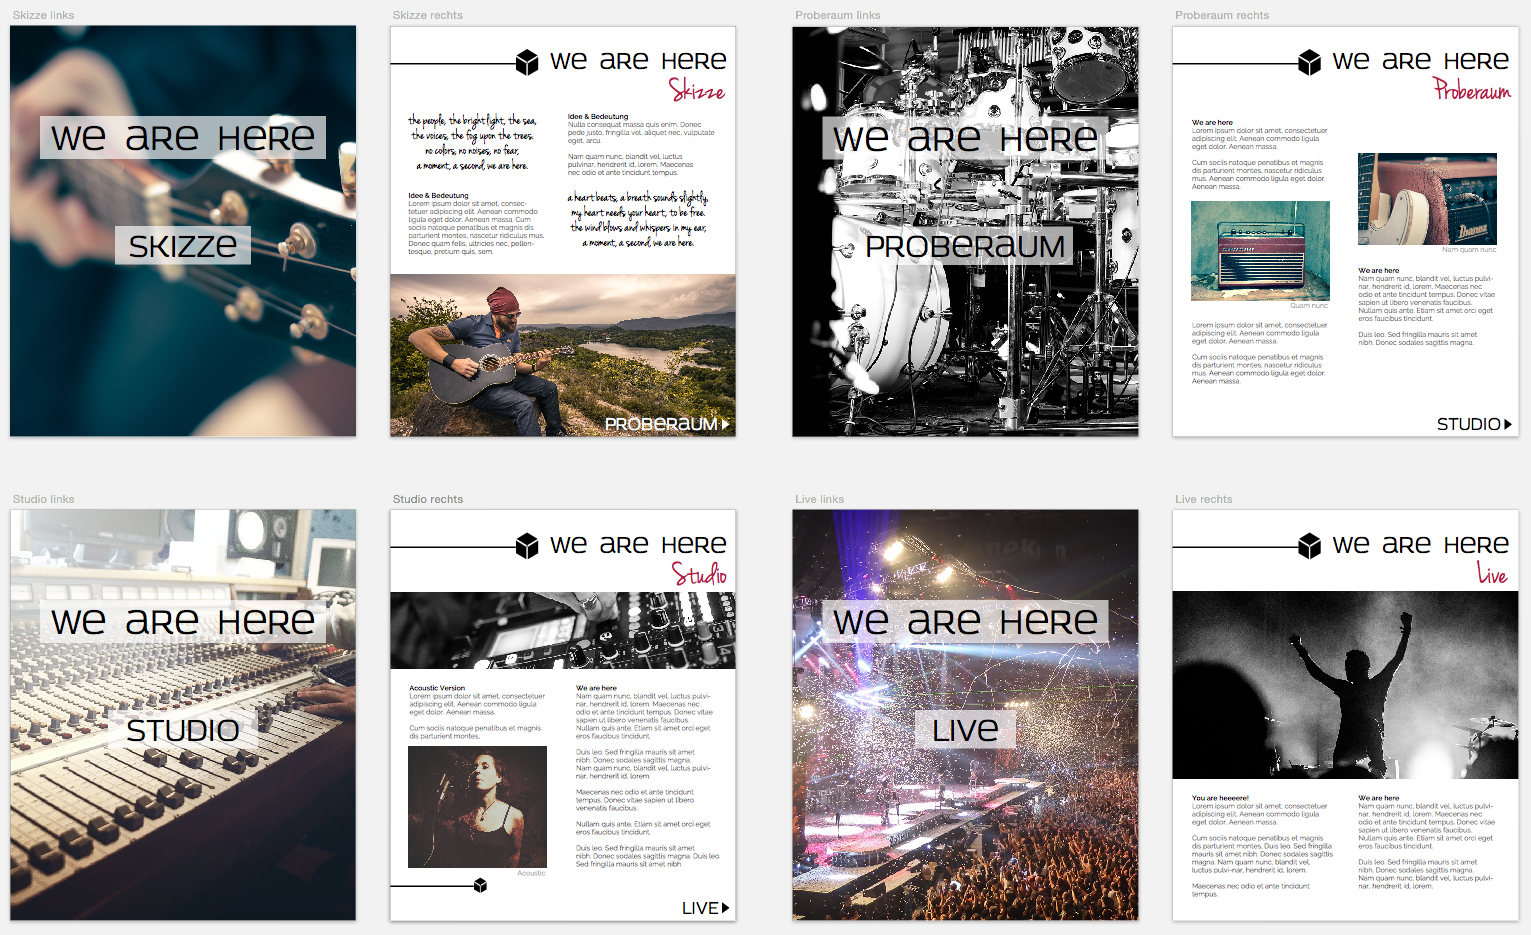
\includegraphics[width=1.0\textwidth]{grafiken/songversions.png}
\caption{}
\end{figure}

\vspace{0.5cm}


%%%%%%%%%%%%



\subsection{Story \& Storyboards}
Für jeden Videoclip wurde eine Story erstellt, die im Anhang einsehbar ist. Für die Visualisierung der Funktionen Multitrack und SongKit wurde zuvor der akustische Ablauf (Reihenfolge des Starten und Stoppens der einzelnen Spuren) in einer Musikproduktionssoftware getestet. Auf ein Storyboard wurde verzichtet, da sich die Kameraeinstellung nicht ändert. Das Buch wird einmal im geschlossenen und im geöffneten Zustand, mit dem jeweils dafür erstellten Layout, für ca. 10 Sekunden aufgenommen. Die auszuführenden Aktionen (Kopfhörer einstecken, Buch aufblättern, Schaltfläche berühren, etc.) erfolgen sequenziell. Alle Funktionen werden von einer Hand ausgeführt. Initial ruht die Hand außerhalb des sichtbaren Bereichs. Bei Ausführung der jeweiligen Funktion  wird die Hand sichtbar und geht nach Ausführung wieder in den nicht sichtbaren Bereich zurück.


\vspace{0.5cm}



%%%%%%%%%%%%%%%%%%%%%%%%%%%%%%%%%%%%
%%%%%%%%%%%%%%%%%%%%%%%%%%%%%%%%%%%%

\section{Webhosting \& Domain}
Um die Website ins verfügbar zu machen, wird ein strategisch sinnvoller Domainname benötigt. Der Domainname soll nah an dem Produkt "Digitales Klangbuch" sein und möglichst kurz, prägnant und verfügbar sein. Folgende Namen wurden auf Verfügbarkeit geprüft:

\begin{itemize}
\item klangbuch.de (belegt, unkonfiguriert)
\item klangbuch.com (belegt, bei Aufruf Fehlermeldung, nicht erreichbar)
\item klangbuch.net (frei)
\item digitales-klangbuch.de (frei)
\item digitales-klangbuch.com (frei)
\item digitales-klangbuch.net (frei)
\end{itemize}

Die Wahl fiel auf die Domain "klangbuch.net", da die verkürzte Version (klangbuch statt digitales-klangbuch) einprägsamer ist. 


%%%%%%%%%%%%%%%%%%%%%%%%%%%%%%%%%%%%
%%%%%%%%%%%%%%%%%%%%%%%%%%%%%%%%%%%%

\section{Konzeption Website}
Um die Realisierbarkeit innerhalb des zeitlichen Rahmens der Bachelorarbeit sicher zu stellen, soll die erste Version des Leitfadens als Website nur die wichtigsten Inhalte abbilden:

\begin{itemize}
\item Einbinden aller erstellten \gls{videoclip}s
\item Erklärungstext zu den erstellten \gls{videoclip}s
\item kurzer Einleitungstext zum digitalen Klangbuch
\end{itemize}

Die Website soll dem Besucher direkt einen Einstieg in das digitale Klangbuch geben. Daher ist es sinnvoll den Startclip als ersten \gls{clip} einzubinden. Das entwickelte Design (s. Kapitel \ref{design}) wird ebenfalls für die Website verwendet. Die Website soll ein reduziertes Design haben, zum digitalen Klangbuch passen und ein reaktionsfähiges\footnote{Reaktionsfähig oder Responsive ist ein Ausdruck aus der Webentwicklung. \gls{responsive} Webdesign bedeutet, dass sich das Layout einer Website auf unterschiedlichen Endgeräten anpasst.} Layout haben. Um den Aufwand der Entwicklung und des Testings möglichst gering zu halten, wurde hierbei die Nutzung eines fertigen Template-Sets in Erwägung gezogen. Für den Fall, dass kein passendes Template gefunden wird, muss eine eigene Entwicklung erfolgen.\\

\textbf{Sprache}\\
Die Website wird komplett in englischer Sprache sein. Dies hat den Vorteil, dass die Website einem internationalen Publikum präsentiert werden kann. Der Begriff "Digitales Klangbuch" bleibt dabei in deutscher Sprache, da dies der Name des Projekts ist.\\

\textbf{Ideenbuch als Titel}\\
Der Leitfaden wird auf der Website selbst als Ideenbuch betitelt. Die im Leitfaden vorgestellten Funktionen sind Ideen, die den KlangKünstler dazu inspirieren sollen, eigene Ideen zu entwickeln. Daher passt der Titel "Ideenbuch" besser, als der Titel "Leitfaden".


%%%%%%%%%%%%%%%%%%%%%%%%%%%%%%%%%%%%
%%%%%%%%%%%%%%%%%%%%%%%%%%%%%%%%%%%%
%%%%%%%%%%%%%%%%%%%%%%%%%%%%%%%%%%%%
%%%%%%%%%%%%%%%%%%%%%%%%%%%%%%%%%%%%
%%%%%%%%%%%%%%%%%%%%%%%%%%%%%%%%%%%%
%%%%%%%%%%%%%%%%%%%%%%%%%%%%%%%%%%%%







\chapter{Umsetzung Leitfaden}
Um den Leitfaden als Website umzusetzen, muss ein geeignetes Template-Set recherchiert und an das entwickelte Design angepasst werden. Wird kein passendes Template-Set gefunden, wird selbst eines entwickelt. Die \gls{videoclip}s müssen gedreht, montiert, in ein internettaugliches Format konvertiert und in die Website eingebunden werden. Es müssen Informations- und Erklärungstexte in englischer Sprache verfasst werden. Die Website muss auf verschiedenen Browsern und Endgeräten getestet werden.


%%%%%%%%%%%%%%%%%%%%%%%%%%%%%%%%%%%%
%%%%%%%%%%%%%%%%%%%%%%%%%%%%%%%%%%%%

\section{Videodreh \& Montage}

\subsection{Videodreh}

\textbf{Kameraperspektive}\\
Die Videoclips sollen das digitale Klangbuch und die Interaktion mit dem Buch zeigen. Damit der Zuschauer sich auf das Wesentliche, das digitale Klangbuch und die vorgestellte Funktion, konzentrieren kann, ist es sinnvoll das Buch aus der Vogelperspektive oder der Aufsicht zu filmen und einen neutralen Hintergrund zu wählen. Es sollen nur die Hände des Nutzers in dem Film, der die Interaktionen durchführt, über das Buch gleitet und Elemente berührt, zu sehen sein.\\

Es wurden Testaufnahmen zur Aufsicht und zur Vogelperspektive gemacht. Die Wahl fiel auf die Kameraperspektive Aufsicht, da diese dem Zuschauer das Gefühl vermittelt, aus seinen Augen auf das Buch zu schauen und es selbst zu benutzen.

\begin{figure}[H]
\centering
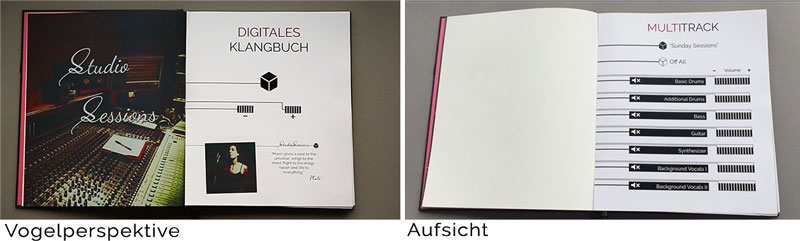
\includegraphics[width=0.8\textwidth]{grafiken/perspektive.jpg}
\caption{Kameraperspektive; Links: Vogelperspektive; Rechts: Aufsicht, vermittelt den Eindruck aus den eigenen Augen auf das Buch zu schauen}
\end{figure}



\textbf{Ausleuchtung, Kameraauswahl \& Probleme}\\
Das zu filmende Buch besteht aus glänzenden, voll- und teil-bedruckten Seiten. Um Reflexionen zu vermeiden, soll das Buch daher nicht direkt, sondern indirekt beleuchtet werden. Auch Schatten, die durch die Bewegung der Hände entstehen, sollen möglichst gering sein.\\

Im ersten Schritt wurde eine DSLR-Kamera für die Aufnahmen der \gls{clip}s verwendet. In einem dunklen Raum mit weißen Wänden und weißer Decke wurde ein Setup mit künstlichem Licht aufgebaut. Es wurden Testaufnahmen zu unterschiedlichen Beleuchtungssituationen gemacht. Trotz indirektem Licht konnten Reflexionen nicht vermieden werden. Durch den hohen Weißanteil auf den Buchseiten wurden die Kanten der Texte im Buch unscharf. Ebenfalls gab es Probleme mit der Farbdarstellung des Buchcovers. Der Druck ist leicht glänzend und schwarz mit pinker Schrift. Die Farbe Schwarz konnte, trotz manuellen Weißabgleichs, nicht ausreichend farbintensiv aufgenommen werden. Durch Einsatz eines Polarisationsfilters, der Licht einer bestimmten Polarisationsrichtung heraus filtert, hätten die Reflexionen absorbiert werden können. Dieser Filter konnte jedoch nicht zum Zeitpunkt der Arbeit beschafft werden.\\
Das Setup wurde dann in einen Raum mit großen Fenstern und natürlichem Licht aufgebaut. Durch das natürliche Licht entstanden deutlich weniger Reflexionen. Jedoch gab es weiterhin Probleme mit unscharfen Kanten und nicht korrekten Farbdarstellungen.\\
Als zweites wurde ein iPhone 6 zur Aufnahme der \gls{clip}s verwendet. Durch die Aufnahme mit dem iPhone 6 und natürlichem Licht, konnten Reflexionen, unscharfe Kanten und Probleme bei der Farbdarstellung signifikant reduziert werden.



\begin{figure}[H]
\centering
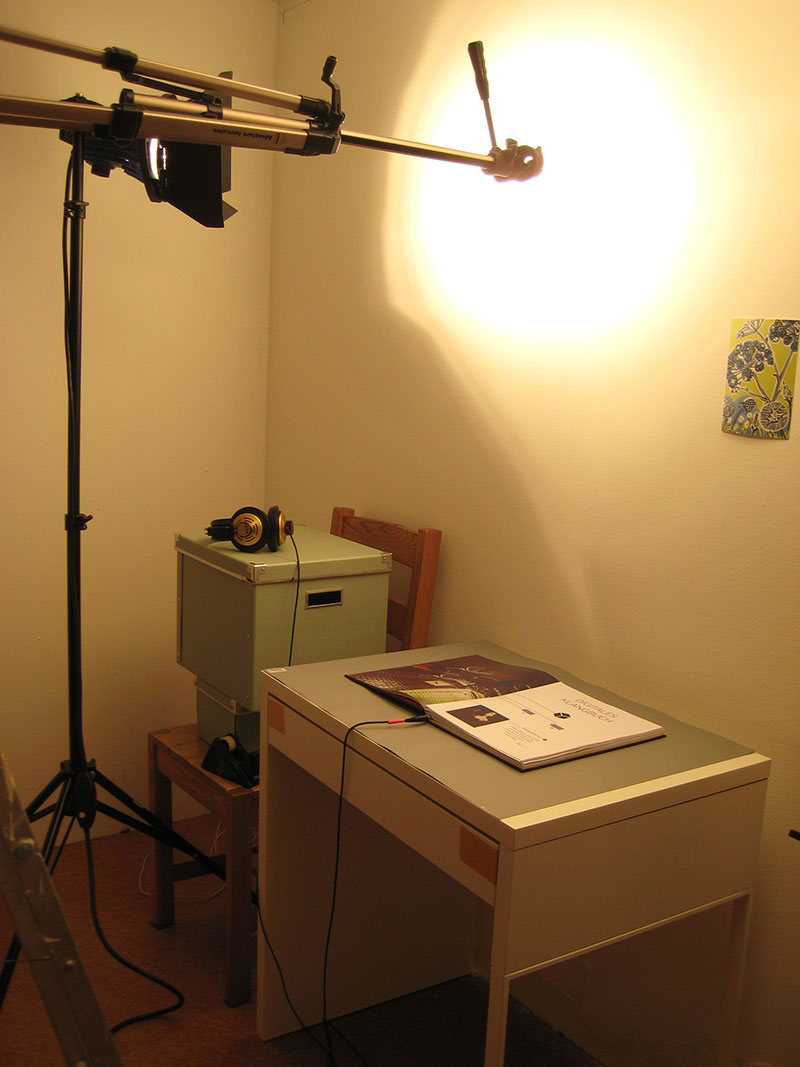
\includegraphics[width=0.3\textwidth]{grafiken/testaufnahmen.jpg}
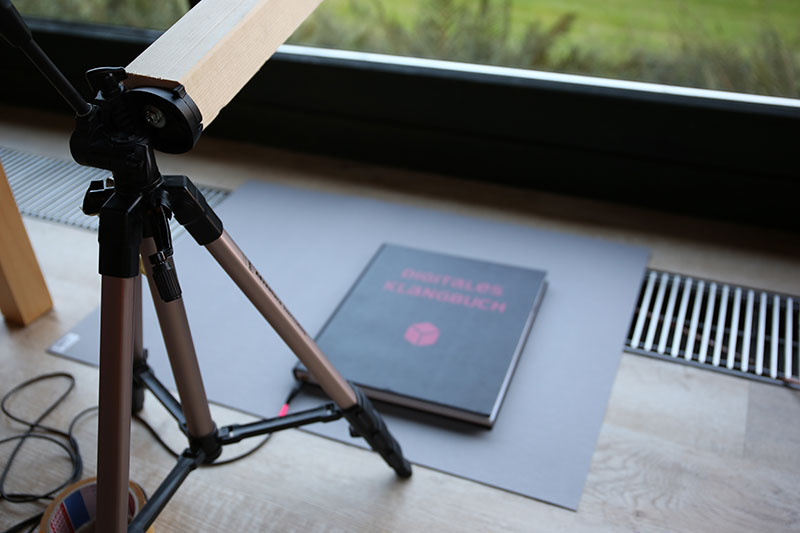
\includegraphics[width=0.4\textwidth]{grafiken/setupII.jpg}
\caption{Setup Testaufnahmen; Links: Künstliches Licht; Rechts: Natürliches Licht}
\end{figure}



\subsection{Montage der \gls{clip}s}
Im Anschluss an den Dreh wurden die einzelnen \gls{clip}s vertont und montiert. Hier bestand die Möglichkeit die Informationen zu den einzelnen \gls{clip}s im Video textuell, z. B. durch eine Bauchbinde, einzublenden oder durch die Aufnahme einer Tonspur zu integrieren. Da in den \gls{clip}s die Interaktion mit Musik dargestellt wird, würde eine weitere Tonspur (Stimme, die die Funktion in dem \gls{clip} erklärt), zu sehr davon ablenken. Der Zuschauer soll sich auf die Veränderungen der Musik konzentrieren, diese sollte nicht durch eine weitere Tonspur belegt werden. Im schlechtesten Fall würde die Tonspur in der Musik untergehen. Daher fiel die Wahl auf das Einblenden von Texten im Video. Um die Konsistenz in allen \gls{clip}s zu bewahren, wird eine Bauchbinde eingesetzt. Diese kann in jedem \gls{clip} an der gleichen Stelle mit selber Größe eingeblendet werden.\\
Als Sprache in den \gls{clip}s wurde Englisch gewählt. So sind die \gls{clip}s international verständlich und müssen, bei Bedarf, nicht erneut in einer anderen Sprache montiert werden.


\begin{figure}[H]
\centering
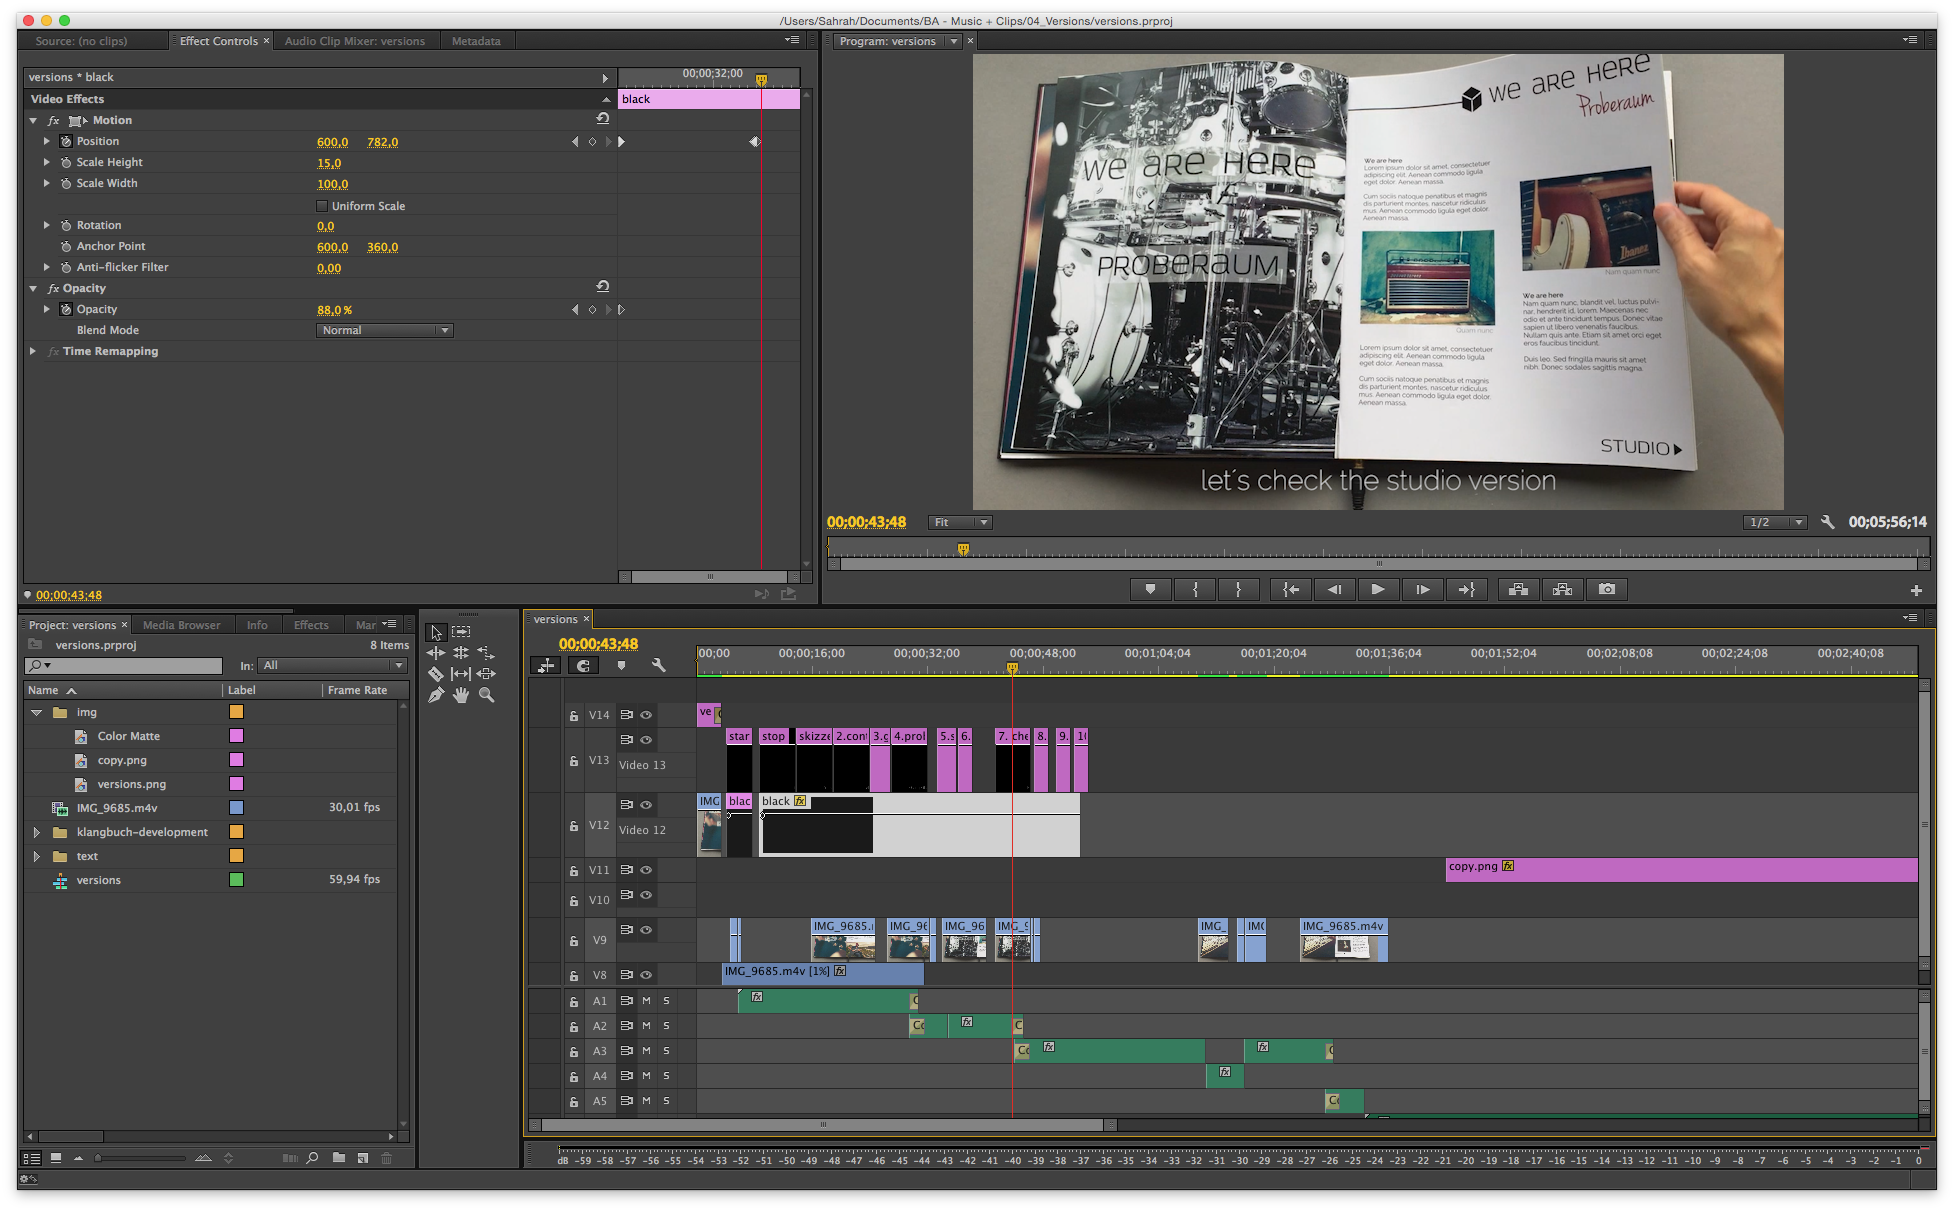
\includegraphics[width=0.8\textwidth]{grafiken/montagefilm.png}
\caption{Montage des \gls{clip}s "Versions"}
\end{figure}


\section{Video-Einbindung}
Die Videos sollten in der Website so eingebunden werden, dass sie von möglichst vielen Browsern auf möglichst vielen Endgeräten abgespielt werden können. Um dieses Ziel zu erreichen, bietet es sich an die Videos über ein Videoportal bereit zu stellen. Videoportale konvertieren die Videos beim Hochladen automatisch in ein browserübergreifendes, webtaugliches Format und betten diese in einen Videoplayer ein. Die Videos sind dann nahezu auf jedem Endgerät abspielbar. Über ein iFrame können die Videos dann in die Website eingebunden werden.\\

\subsection{Auswahl Video-Portal}
Der Video-Kanal muss für die Bachelorarbeit folgende Kriterien erfüllen:

\begin{itemize}
\item Anbieten aller benötigten Funktionen zu einem möglichst geringen Preis
\item Hochladen von mind. vier Videos
\item Möglichkeit zur Einbindung der Videos in eine Website
\item Möglichkeit die Videos nicht zu listen\footnote{Videos nicht listen: Das Hochladen von Videos in Videoportalen bedeutet, dass sie für jeden Internetnutzer sichtbar sind. Durch das Nichtlisten sind die hochgeladenen Videos nicht frei zugänglich, sondern können nur über eine bestimmte URL erreicht werden. Da das Gesamtprojekt "Digitale Klangbuch" noch in der Entwicklung ist, sollten die Videos zum aktuellen Zeitpunkt nicht für jeden frei zugänglich sein.}
\end{itemize}


Das bekannteste Videoportal ist YouTube\footnote{YouTube: \url{http://www.youtube.com}}\cite{statYT}. YouTube erfüllt alle genannten Kriterien und bietet diese Funktionen zudem kostenlos an.\\
Eine Alternative ist das Videoportal Vimeo\footnote{Vimeo: \url{http://www.vimeo.com}}. Anders als bei YouTube ist das Hochladen von Videos bei Vimeo nur gestattet, wenn diese selbst produziert sind und alle erforderlichen Rechte bei einem liegen. Damit richtet sich Vimeo eher an Künstler und Filmproduzenten, während YouTube keine spezielle Zielgruppe hat.\cite{chip} Das Nichtlisten von Videos ist bei Vimeo nur mit einer Pro-Mitgliedschaft für 159 \euro /Jahr möglich, weshalb Vimeo nicht alle Kriterien erfüllt. Da das digitale Klangbuch noch in der Entwicklung ist, sollten die Videos zum aktuellen Zeitpunkt nicht für jeden frei zugänglich sein. Der Videokanal wird auf YouTube erstellt. Für die Zukunft sollte jedoch auch ein Videokanal bei Vimeo eingerichtet werden.\\

Der Video-Kanal ist unter folgendem Link erreichbar:\\\url{https://www.youtube.com/channel/UCJ_SsBh-EhDPPo9xxOF2MVQ}\\
Die Videoclips können ebenfalls von der CD, die der gebundenen Ausgabe der Bachelorarbeit beiliegt, abgespielt werden.


\begin{figure}[H]
\centering

\includegraphics[width=0.8\textwidth]{grafiken/youtubekanal.png}
\caption{YouTube Kanal "Digitales Klangbuch"}
\end{figure}

%%%%%%%%%%%%%%%%%%%%%%%%%%%%%%%%%%%%
%%%%%%%%%%%%%%%%%%%%%%%%%%%%%%%%%%%%

\section{Website}

Für die Entwicklung der Website wurden fertige Template-Sets recherchiert. Das Template-Set soll folgenden Anforderungen entsprechen:\\

\textbf{Inhalte einbinden}\\
Das Einbinden von Texten, Grafiken und Videos soll möglich sein.\\

\textbf{Leicht verständlich \& schlicht}\\
Das Template-Set soll den Aufwand der Entwicklung und des Testings der Website möglichst gering halten. Daher soll es vom Aufbau und Einstieg in die Entwicklung leicht verständlich und schlicht sein.\\

\textbf{\gls{responsive}}\\
Das Template-Set soll responsive aufgebaut sein. Neu hinzugefügte Elemente sollen ebenfalls problemlos responsive eingebunden werden können.\\

\textbf{Editierbar- \& Erweiterbarkeit}\\
Das Template-Set soll einfach editierbar und erweiterbar sein. HTML-, PHP-, Javascript- und \Gls{stylesheet}-Dateien sollen verändert werden können. Das erstellte Design mit Farben, Schriften, Logos soll in das Template-Set integriert werden können.\\

\textbf{Lizenzfrei}\\
Um Kosten zu vermeiden, soll das Template-Set möglichst lizenzfrei sein.\\


Die Wahl fiel auf ein \gls{onepager} Template-Set von "HTML5 UP"\footnote{HTML5 UP: \url{http://www.html5p.net}}. Der Vorteil an einem \gls{onepager}  liegt darin, dass alle Informationen, Funktionen und Videos auf einer Seite ohne Navigation zu finden sind. Durch Scrolling der Seite wird der Nutzer in eine bewusst gesteuerte Reihenfolge durch die Inhalte der Seite geführt.


\subsection{Anpassung Website}
Das \Gls{stylesheet} der Webseite wurde an die Farben und Schriften des entwickelten Designs angepasst. Das Einbinden der Schrift Oxygen konnte über die Api von Google-Font erfolgen.

\begin{lstlisting}
<link href='https://fonts.googleapis.com/css?family=Oxygen:400,300,700'
rel='stylesheet' type='text/css'>
\end{lstlisting}

\vspace{0.5cm}

Die Schrift Azoft musste separat hochgeladen und über das \Gls{stylesheet} eingebunden werden.

\begin{lstlisting}
@font-face{
	font-family: 'azoft';
	src: url("../fonts/azoft-sans.ttf");
}

@font-face{
	font-family: 'azoft';
	src: url("../fonts/azoft-sans-bold.ttf");
	font-weight: bold;
}
\end{lstlisting}


Das Template-Set berücksichtigt nicht das responsive Einbinden von Videos. Dies ließ sich jedoch über einen Open-Source \Gls{stylesheet} Code realisieren:

\begin{lstlisting}
// Embeds responsive
// Credit: Nicolas Gallagher and SUIT CSS.

.embed-responsive {
  position: relative;
  display: block;
  height: 0;
  padding: 0;
  overflow: hidden;

  .embed-responsive-item,
  iframe,
  embed,
  object,
  video {
    position: absolute;
    top: 0;
    left: 0;
    bottom: 0;
    height: 100%;
    width: 100%;
    border: 0;
  }
}

// Modifier class for 16:9 aspect ratio
.embed-responsive-16by9 {
  padding-bottom: 56.25%;
}
\end{lstlisting}


\subsection{Testen der Website}
Die Website wurde auf verschiedene Browser und Endgeräte getestet und angepasst.\\
\textbf{Getestete Browser}: Google Chrome, Safari, Firefox.\\
\textbf{Getestete Endgeräte}: Apple iPad, Apple iPhone 6, Google Nexus\\


Screenshots zur Webseite können im Anhang eingesehen werden.
Die Website ist unter folgender URL zu erreichen: \url{http://www.klangbuch.net}


%TODOs:\\
%\begin{itemize}

%\item Glossar vervollständigen
%\item Was ist eigentlich ein Erlebnis?
%\item Beispiele für Gesamtkunstwerk\\Pink Floyd - Pulse 2 Album ?\\Mogwai - Rave Tapes?
%\item Überall Klangbuch Schreibweise checken
%\item Ganz am Ende die Bib + Glossar neu erstellen + alle Begriffe im Dok hinzufügen

%\end{itemize}











%%!TEX root = ../PP.tex

\newcommand{\fFunktionen}{040_funktionen}

\part{Der Leitfaden}

\textbf{Der Leitfaden - Beschreibung}\\
Dieser Teil erläutert die Möglichkeiten und Grenzen des digitalen Klangbuchs. Es werden Darstellungsmöglichkeiten und Funktionen erarbeitet. Arten von Leitfäden werden diskutiert und ein Leitfaden konzipiert und umgesetzt.

%!TEX root = ../PP.tex

%TODO: 

\chapter{Möglichkeiten und Grenzen des digitalen Klangbuchs}\label{moeglichkeiten}

Bevor ein Leitfaden und Funktionen für das digitale Klangbuch entwickelt werden können, müssen zuvor die Möglichkeiten und Grenzen des digitalen Klangbuchs erläutert werden. Im Folgenden wird das digitale Klangbuch mit seinen technischen Möglichkeiten und Grenzen kurz skizziert.


%%%%%%%%%%%%
%%%%%%%%%%%%

\section{Technik im digitalen Klangbuch}

Im Praxisprojekt wurden unterschiedliche Realisierungsansätze vorgestellt. Die Ansätze präsentierten dabei verschiedene Technologien und Möglichkeiten zum Aufbau des Buches. Um den Rahmen der Bachelorarbeit nicht zu sprengen, beschränkt sie sich auf folgende Technologien und Hilfsmittel, die bei der Funktionsentwicklung und der Entwicklung des Leitfadens im digitalen Klangbuch eingesetzt werden:


\begin{itemize}
\item{Leitende Tinte}
\item{Leitender Kleber}
\item{Gedruckte Elektronik}
\item{SMD-LEDs}
\end{itemize}

\textbf{Leitende Tinte} ist eine Flüssigkeit, mit der sich funktionierende Stromkreise auf Papier zeichnen und drucken lassen. Aufgrund des körpereigenen Widerstands ist die Tinte berührungsempfindlich. Dadurch lassen sich Bedienelemente direkt auf das Papier drucken.\\

Unter \textbf{gedruckte Elektronik} versteht man elektronische Bauteile, die über ein spezielles Verfahren auf ein Trägermaterial aufgedruckt werden können. Ein zentraler Ansatz im digitalen Klangbuch ist die Erkennung der Seite, auf der sich der Hörer gerade befindet. Dadurch lassen sich Funktionen, die nur auf einer bestimmten Seite möglich sind, steuern. Z. B. das automatische Starten eines Songs, sobald eine spezielle Seite umgeblättert wird. Ein gedruckter Sensor ist für die Seitenerkennung notwendig. Der Sensor ist nicht sichtbar zwischen zwei Seiten eingebettet und taucht deshalb nicht in den Skizzen der Funktionsbeschreibungen auf.\\


\textbf{Leitender Kleber} ist ein Klebstoff, der Strom leitet. Damit lassen sich Elemente, die an einen Stromkreis angeschlossen werden müssen, über den Klebstoff integrieren, z. B. SMD-LEDs. Der Kleber wiederum wird mit leitender Tinte verbunden.\\


\textbf{SMD-LEDs} sind winzig kleine LEDs, die ohne Drähte auskommen. Sie können mit dem leitenden Kleber direkt auf das Papier des Klangbuchs aufgeklebt werden. Die kleinste Bauform misst eine Größe von 1,0 x 0,5 x 0,45 mm.\\


%%%%%%%%%%%%


\section{Aufbau Digitales Klangbuch}
In Abbildung \ref{fig:aufbauBuch} ist der Aufbau des digitalen Klangbuchs skizziert: Im hinteren Buchdeckel ist die Technik zur Steuerung eingebettet (1). Der Buchrücken (3) ist mit den Komponenten im Buchdeckel verbunden. Auf den einzelnen Seiten des Buches können mit leitender Tinte berührungsempfindliche Elemente (2.1) gedruckt und mit leitendem Kleber SMD-LEDs (2.2) integriert werden. Jede SMD-LED und jedes berührungsempfindliche Element muss mit leitender Tinte mit dem Buchrücken verbunden werden.


\begin{figure}[H]
\centering
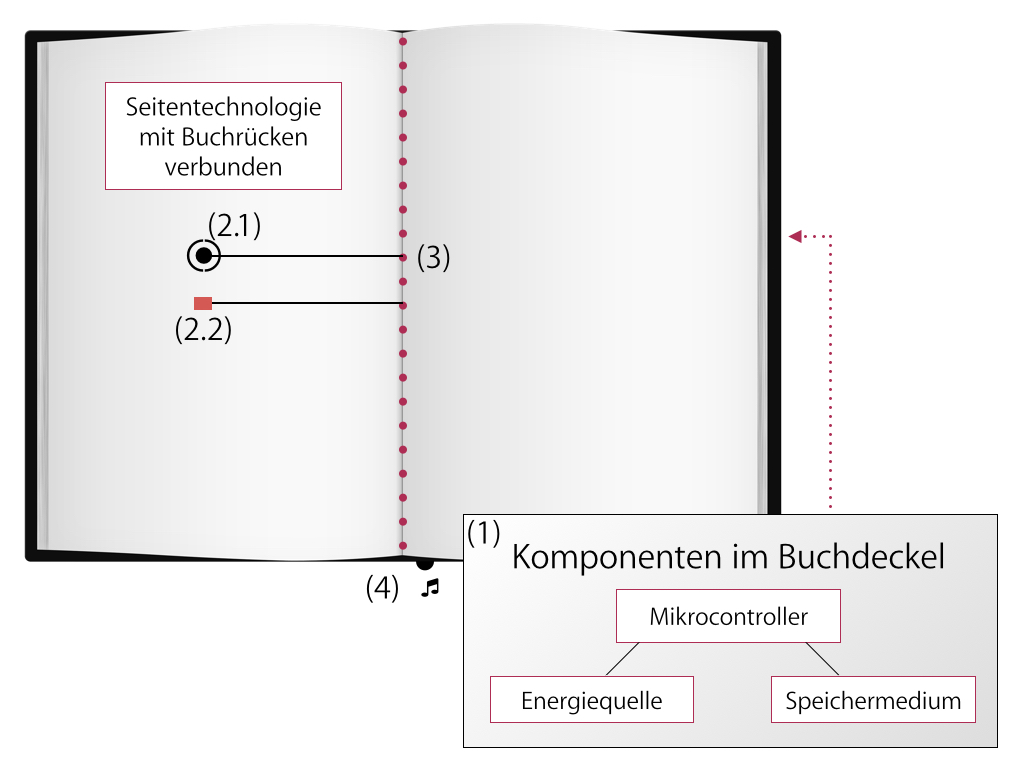
\includegraphics[width=1.0\textwidth]{grafiken/aufbau-klangbuch.jpg}
\caption{Aufbau des digitalen Klangbuchs: (1) Technik im Buchdeckel, (2.1) berührungsempfindliches Element, (2.2) SMD-LED, (3) Buchrücken, (4) Audioausgang }
\label{fig:aufbauBuch}
\end{figure}


\section{Möglichkeiten \& Grenzen}

\subsection{Möglichkeiten}
Durch den Einsatz der zuvor beschriebenen Technik, ist es möglich Audiodaten abzuspielen, SMD-LEDs anzusteuern und Interaktionen auszuwerten (Berührung eines berührungsempfindlichen Elements). Die Auswertung der Interaktion kann für den Hörer in zwei Formen sichtbar gemacht werden:\\
1. Eine Interaktion bewirkt eine eine akustische Veränderung: ein Klang ertönt oder verstummt (z. B. wird ein Song beim Berühren eines bestimmten Elements gestartet).\\
2. Eine Interaktion bewirkt eine visuelle Veränderung: eine oder mehrere SMD-LEDs beginnen zu leuchten, verdunkeln, blinken oder ändern ihren Farbwert.

\subsection{Grenzen}
Berührungsempfindliche Elemente werden mit spezielle, leitende Tinte auf die Seiten des Buches gedruckt. Diese Elemente und jede integrierte SMD-LED werden durch Linien aus gedruckter leitender Tinte mit dem Buchrücken verbunden. Bei der Erstellung der Layouts müssen diese Elemente und Linien berücksichtigt werden. Dabei ist auch zu beachten, dass die Linien ebenfalls auf Berührung reagieren und sie sich auch gegenseitig nicht berühren dürfen.



%%%%%%%%%%%%%%%%%%%%%%%%%%%%%%%%%%%%%%%%%%%%%%%%%%%%%%%%%%%%%%%%%%%%%%%%%%%%%%%%%%%%%%%%%%%%%%%%
%%%%%%%%%%%%%%%%%%%%%%%%%%%%%%%%%%%%%%%%%%%%%%%%%%%%%%%%%%%%%%%%%%%%%%%%%%%%%%%%%%%%%%%%%%%%%%%%
%%%%%%%%%%%%%%%%%%%%%%%%%%%%%%%%%%%%%%%%%%%%%%%%%%%%%%%%%%%%%%%%%%%%%%%%%%%%%%%%%%%%%%%%%%%%%%%%
%%%%%%%%%%%%%%%%%%%%%%%%%%%%%%%%%%%%%%%%%%%%%%%%%%%%%%%%%%%%%%%%%%%%%%%%%%%%%%%%%%%%%%%%%%%%%%%%
%%%%%%%%%%%%%%%%%%%%%%%%%%%%%%%%%%%%%%%%%%%%%%%%%%%%%%%%%%%%%%%%%%%%%%%%%%%%%%%%%%%%%%%%%%%%%%%%


\chapter{Darstellungs- und Funktionsmöglichkeiten}\label{funktionen}

Das digitale Klangbuch spricht den haptischen, visuellen und akustischen Sinn an. Im Folgenden werden Ideen und Funktionen entwickelt. Diese werden in folgende Bereiche unterteilt: Interaktion (haptische Wahrnehmung), Darstellungsmöglichkeiten (visuelle Wahrnehmung) und Akustik (auditive Wahrnehmung).

%%%%%%%%%%%%
%%%%%%%%%%%%
%%%%%%%%%%%%

\section{Interaktion}
Das digitale Klangbuch ermöglicht es dem Hörer interaktiv mit dem Buch und dessen Inhalte zu agieren.

\subsection{Berührungsempfindliche Elemente}
Elemente, die mit leitender Tinte gedruckt und mit dem Buchrücken verbunden wurden, sind berührungsempfindlich. Bei Berührung können sie eine Funktion auslösen, z. B. das Starten eines Songs. Durch logische Verknüpfungen ist es auch möglich berührungsempfindliche Elemente miteinander zu verketten. Ein Beispiel: Berührung von Element A löst Funktion a aus. Berührung Element B, löst Funktion b aus. Berührung von Element A und B zu gleicher Zeit, löst Funktion c aus.

\subsection{Umblättern einer Seite}
Die Seiten des digitalen Klangbuchs sind mit Sensoren ausgestattet. Wird eine Seite umgeblättert, registriert der Sensor auf welcher Seite sich der Hörer befindet. Es kann dann eine Funktion ausgelöst werden, z. B. das Starten eines Songs.


%%%%%%%%%%%%
%%%%%%%%%%%%
%%%%%%%%%%%%

\section{Darstellungsmöglichkeiten}

Im digitalen Klangbuch ist an Inhalten alles möglich, was ein herkömmliches Buch bietet: Raum für Geschichten, Bilder, Illustrationen, Texte, etc. Kombiniert mit der Technik, den Interaktionsmöglichkeiten und der Musik bzw. Audioinhalten, lassen sich unzählige, neuartige Inhalte generieren. Denkbar wären z. B.:

\begin{itemize}
\item Entstehungsgeschichte des Musikers / der Band, begleitet von Musik, Audiokommentaren, etc.
\item Informationen und Geschichten über den Musiker / der Band
\item Bedeutung, die hinter einem ausgewählten Songs steht
\item Entstehungsprozess eines ausgewählten Songs
\item bisherige Veröffentlichungen, \gls{remix}e, etc.
\item Lyriktexte der Songs
\item Fotos des Musikers / der Band
\item Zeichnungen, Bilder, Illustrationen
\end{itemize}

Die Seiten des digitalen Klangbuchs bestehen aus gängigem Fotopapier. Sie können nach Wünschen des Künstlers farbig bedruckt werden. So können Fotos, Grafiken, künstlerische Werke, Texte, etc. auf die Seiten gedruckt werden. Es ist ebenfalls möglich spezielle Techniken aus der Buchkunst zu integrieren, z. B. Pop Up´s\footnote{Pop Up Kunst bezeichnet Elemente, die durch eine besondere Falttechnik räumlich herausspringen (pop up).} (s. Abbildung \ref{fig:Popup}) und diese ebenfalls mit leitender Tinte und SMD-LEDs zu kombinieren (s. Abbildung \ref{fig:PopupLED}.\\


\begin{figure}[H]
\centering
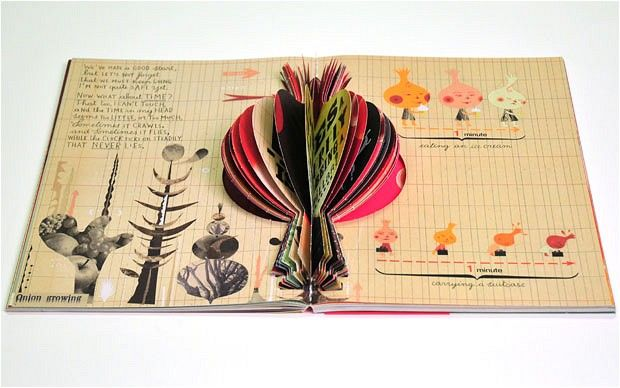
\includegraphics[width=0.8\textwidth]{grafiken/popup.jpg}
\caption{Pop Up Kunst in einem Buch.\\Foto: The Onion’s Great Escape by Sara Fanelli, Portia Webb, \url{http://www.telegraph.co.uk/culture/books/children_sbookreviews/9682987/Books-for-Christmas-childrens-books.html} }
\label{fig:Popup}
\end{figure}


\subsection{Leuchtende Elemente}
Durch eingesetzte SMD-LEDs ist es möglich Veränderungen visuell anzuzeigen und so Informationen zu transportieren. Eine SMD-LED kann blinken, leuchten und die Farbe wechseln. So können z. B. SMD-LEDs auf einer Zeitleiste angeordnet werden, welche dem Hörer durch Blinken anzeigt, an welcher Stelle sich der Song gerade befindet.


\begin{figure}[H]
\centering
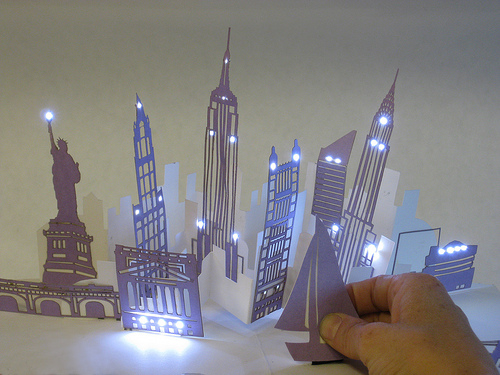
\includegraphics[width=0.5\textwidth]{grafiken/popupled.jpg}
\caption{Pop Up Kunst mit LEDs.\\Foto: Electronic Popables, high-low tech, \url{http://highlowtech.org/?p=5} }
\label{fig:PopupLED}
\end{figure}


\subsection{Grenzen im Layout}
Berührungsempfindliche Elemente werden mit spezieller, leitender, schwarzer Tinte auf die Seiten des Buches gedruckt. Diese Elemente und jede integrierte SMD-LED werden durch Linien aus gedruckter leitender Tinte mit dem Buchrücken verbunden. Bei der Erstellung der Layouts müssen diese Elemente und Linien berücksichtigt werden. Dabei ist auch zu beachten, dass die Linien ebenfalls auf Berührung reagieren und sie sich auch gegenseitig nicht berühren dürfen.

\begin{figure}[H]
\centering

\includegraphics[width=0.8\textwidth]{grafiken/bspklangbuch.png}
\caption{Beispiel Layout eines digitalen Klangbuchs: Berührungsempfindliche Elemente werden mit Linien aus leitender Tinte mit dem Buchrücken verbunden. Die Linien dürfen sich nicht kreuzen.}
\end{figure}




%%%%%%%%%%%%
%%%%%%%%%%%%
%%%%%%%%%%%%

\section{Akustik}
Ein herkömmliches CD-/DVD-/Blueray-Album bietet dem Fan in manchen Fällen auch Bonusmaterial. Das Bonusmaterial ist vor allem auf der CD begrenzt und besteht oft nur aus einem zusätzlichen Song, z. B. ein \gls{remix}. Mit dem digitalen Klangbuch soll das herkömmliches Album um Funktionen und Inhalte erweitert werden. In diesem Kapitel werden Funktionen und Ideen vorgestellt, die vor allem den akustischen Sinn des Fans ansprechen sollen. 


\subsection{Audio abspielen}
Die grundlegendste Funktion ist die Möglichkeit ein Audiostück zu starten, zu stoppen, zu pausieren und die Lautstärke zu regeln.\\


\textbf{Unterschied zum herkömmlichen Album}\\
Der Hörer berührt im digitalen Klangbuch Elemente, die auf eine Papierseite aufgedruckt sind. Dadurch wird der haptische und der auditive Sinn angesprochen.\\

\textbf{Erweiterte Funktionsmöglichkeit}\\
Die Veränderungen können durch SMD-LEDs angezeigt werden, wodurch auch eine visuelle Änderung wahrgenommen werden kann.


%%%%%%%%%%%%


\subsection{Sprachwahl}
Die Gesangsspur eines Songs kann über eine Auswahl in einer anderen Sprache abgespielt werden.\\


\textbf{Unterschied zum herkömmlichen Album}\\
Ein Song, der Gesang oder Sprache enthält, wird für gewöhnlich in einer ausgewählten Sprache gesungen / gesprochen. Selten hat der Hörer die Möglichkeit den Song auch in einer anderen Sprache zu hören. Der KlangKünstler kann dem Hörer eine Auswahl an Spuren in unterschiedlicher Sprache anbieten.\\


\textbf{Weiteres Nutzungsszenario}\\
Dem Hörer kann es möglich sein die Gesangsspur durch eine eigene zu ersetzen.



%%%%%%%%%%%%


\subsection{Interview}
Statt eines Songs, können auch Interviews des KlangKünstler hinterlegt werden.\\


\textbf{Unterschied zum herkömmlichen Album}\\
Im Gegensatz zu einem kleinformatigem \gls{booklet}, können die Interviews im großformatigen digitalen Klangbuch ausführlich grafisch begleitet werden. So kann der Fan zu vielen Details im Interview visuell bedient werden.\\


\textbf{Weiteres Nutzungsszenario}\\
Anhand von SMD-LEDs können visuelle Inhalte des Buches (Bilder, Texte, etc.) passend zu den Stellen des Interviews deutlich gemacht werden.



%%%%%%%%%%%%


\subsection{Equalizer - Presets}
Eine weitere Grundfunktion, die in gängigen Geräten zum Abspielen von Audio enthalten ist, ist ein Equalizer. Er dient dazu um den Klang an die eigenen Wünsche anzupassen: Höhen, Tiefen, etc. Das digitale Klangbuch kann hierzu sogenannte Presets, parametrische Voreinstellungen des Equalizers, anbieten.\\

\textbf{Unterschied zum herkömmlichen Album}\\
Der Hörer berührt im digitalen Klangbuch Elemente, die auf einer Papierseite aufgedruckt sind. Dadurch wird der haptische und der auditive Sinn angesprochen.\\

\textbf{Erweiterte Funktionsmöglichkeit}\\
Die Veränderungen können durch SMD-LEDs angezeigt werden, wodurch auch eine visuelle Änderung wahrgenommen werden kann.


%%%%%%%%%%%%

\subsection{\gls{remix}e}
Der Hörer kann sich zu einem Song verschiedene \gls{remix}e anhören.\\

\textbf{Unterschied zum herkömmlichen Album}\\
Im Gegensatz zu einem kleinformatigem \gls{booklet}, können die \gls{remix}e im großformatigen digitalen Klangbuch ausführlich grafisch begleitet werden.


%%%%%%%%%%%%
%%%%%%%%%%%%
%%%%%%%%%%%%


\subsection{Multitrack}
Multitrack bedeutet zu deutsch "Mehrspur". Es bietet die Möglichkeit einen Song in mehreren, separaten Spuren abzuspielen und diese bei Bedarf einzeln stummzuschalten, auszutauschen oder zu bearbeiten.\\

\textbf{Unterschied zum herkömmlichen Album}\\
Der Hörer hat hier die Möglichkeit einzelne Spuren stumm zu schalten und die Lautstärke der Spuren einzeln zu verändern.\\

\textbf{Erweiterte Funktionsmöglichkeit}\\
Dem Hörer kann es möglich sein eine der Spuren, z. B. die Gesangsspur, durch eine eigene zu ersetzen.


%%%%%%%%%%%%


\subsection{SongKit}
Als SongKit ist in diesem Kontext ein Bausatz zu verstehen, der verschiedene \gls{loop}s einer Klangspur zur Verfügung stellt. Die Idee dahinter ist, ein Musikstück des Albums in seine Spuren zu teilen - beispielsweise in Bass, Drums, Melodie, Gesang - und diese in einer Dauerschleife abspielen zu lassen. Zu jeder Spur gibt es Alternativen, die ausgewählt werden können. So kann der ursprüngliche Song verändert werden.\\


\textbf{Unterschied zum herkömmlichen Album}\\
In der Produktionsphase eines Songs verändert sich der Song von der Idee bis zum fertigen Song. Andere Versionen des Songs, z. B. mit einer anderen Basspur, bekommt der Musikfan nahezu nie zu hören. Durch das SongKit im Klangbuch können diese Versionen integriert werden. Dabei kann der Hörer selbst bestimmen, welche Spuren er zusammen mischt.\\


\textbf{Weiteres Nutzungsszenario}\\
Das SongKit kann unabhängig vom Album eine Auswahl an \gls{loop}s bereit stellen. Das heißt, die \gls{loop}s müssen nicht zwingend einen Bezug zu dem Album oder einem Song haben. Die KlangKünstler können einen Baukasten mit passenden \gls{loop}s zusammen stellen, die der Hörer dann nach seinen Wünschen zu einem Song-\gls{loop} zusammen stellt.



%%%%%%%%%%%%


\subsection{Audiokommentare}
Zu einem Song können Audiokommentare hinterlegt werden, die sich der Hörer bei Bedarf anhören kann. Die Audiokommentare können in einer Timeline, passend zum Song, hinterlegt werden. Aktiviert der Hörer die Audiokommentare, reduziert sich die Lautstärke des bereits laufenden Songs, sodass die entsprechenden Audiokommentare an den passenden Stellen erklingen können. \\


\textbf{Unterschied zum herkömmlichen Album}\\
Audiokommentare sind selten in einem gewöhnlichen Musikalbum zu finden.\\


\textbf{Weiteres Nutzungsszenario}
\begin{itemize}
\item Variation 1: Audiokommentare können über einzelne \gls{button}s individuell gestartet werden.
\item Variation 2: Die Kommentare können als Texte im Buch hinterlegt werden. Erreicht der laufende Song einen Audiokommentar, leuchtet eine dazu platzierte SMD-LED auf. Ein ähnliches Konzept findet sich auf Soundcloud\footnote{Soundcloud ist ein Online-Musikdienst für Musiker zum Anbieten von Audiodateien. Fans können auf der Zeitleiste eines Songs zu jeder Sekunde einen Kommentar hinterlassen.}.
\end{itemize}


%%%%%%%%%%%%


\subsection{Interaktiver Song}
In interaktiven Videos\footnote{Interaktives Videobeispiel: Ink von Colplay\cite{CO}} ist es möglich den Handlungsstrang zu beeinflussen. Der Verlauf eines Songs kann über das digitale Klangbuch ebenfalls durch den Hörer bestimmt werden. Ein Beispiel dazu wird in der Skizze - Abbildung \ref{fig:abb1} veranschaulicht.\\
Beim Öffnen der Seite wird der Song automatisch gestartet. Die Zeitleiste (a) symbolisiert die Länge des Songs. Der Hörer hat nun die Möglichkeit den Verlauf des Songs, während dieser bereits spielt, zu ändern. Dazu wurde der Song in drei Bereiche geteilt (Minute 0:30, 1:30 und 2:30). Diese Bereiche werden im Folgenden "Kapitel" genannt.\\ 

Der Hörer hat die Möglichkeit in jedem Kapitel den Verlauf des Songs zu verändern:
\begin{itemize}
\item Kapitel 1: Der Song kann eine dramatische, eine ruhige oder eine rätselhafte Richtung einschlagen.
\item Kapitel 2: Die Gesangsstimme kann männlich, weiblich oder die eines Kindes sein.
\item Kapitel 3: Das Ende des Songs kann mitbestimmt werden - ein fröhliches, ein zerstörtes oder überhaupt kein Ende, sodass der Song von neuem beginnt.
\end{itemize} 

SMD-LEDs (b) zeigen dem Hörer an, wie lang es ihm möglich ist den Verlauf für dieses Kapitel zu ändern. Solange die SMD-LED in einem der Kapitel leuchtet, kann der Hörer den Verlauf bestimmen.


\begin{figure}[H]
\centering
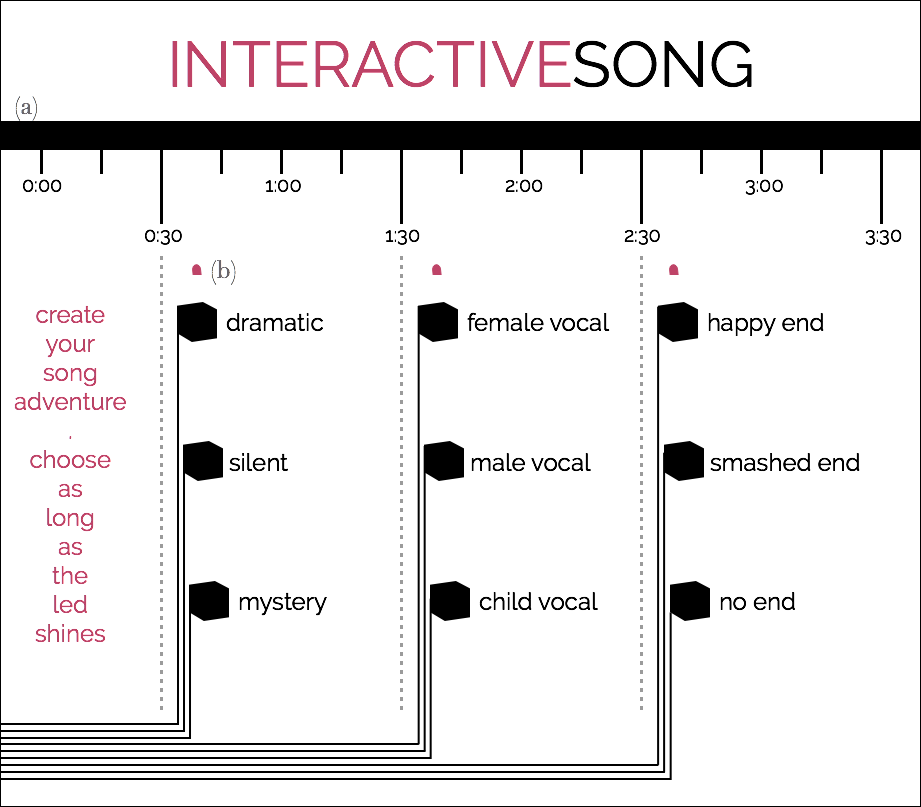
\includegraphics[width=1.0\textwidth]{grafiken/function_interactivesong.png}
\caption{Beispiel-Skizze Interaktiver Song im digitalen Klangbuch}
\label{fig:abb1}
\end{figure}


\textbf{Unterschied zum herkömmlichen Album}\\
Interaktive Songs sind nicht neu. Auf einem Album kann diese Idee jedoch nicht verwirklicht werden. Im Internet gibt es Beispiele zu interaktiven Songs z. B. auf dem Videoportal YouTube\footnote{Interaktiver Song auf YouTube: \url{https://www.youtube.com/watch?v=OtcpO4vipNU}} und dem Storytelling Tool interlude\footnote{interlude:\url{http://blog.interlude.fm/}}.\\


\textbf{Weiteres Nutzungsszenario}
\begin{itemize}
\item Ideenbeispiel 1: Der Interaktive Song kann auf mehrere Seiten im Buch ausgeweitet werden. So kann der Inhalt der Seiten auf jeden "Handlungsstrang" angepasst werden.
\item Ideenbeispiel 2: Der Song kann eine Geschichte erzählen, sowohl grafisch, als auch über den Songtext. Je nach gewählten Handlungsstrang, kann die Geschichte eine andere Wendung nehmen, der Songtext ändert sich. Die verschiedenen Songtexte können im Klangbuch abgebildet und vom Hörer mitgelesen werden.
\end{itemize}



%%%%%%%%%%%%


\subsection{Entstehungsgeschichte Song - "Versions"}
Die Entstehungsgeschichte eines Songs, im Folgenden auch "Versions" genannt, kann im digitalen Klangbuch nicht nur durch Texte und passende Bilder erzählt werden. Der Hörer kann auch in die verschiedenen Versionen, die ein Song von der Idee hin zu einer Live-Version durchläuft, hinein hören. Beispielstationen bei der Entwicklung eines Songs sind folgende:

\begin{itemize}
\item Skizze: Die erste Idee, die auf einem Klavier oder einer Gitarre entsteht
\item Proberaumversion: Die weiter verarbeitete Idee, die mit der Band im Proberaum verfeinert wird
\item Studioversion: Der Song wird professionell in einem Studio aufgenommen
\item Live-Version: Eine Aufnahme, die auf einem Live-Konzert mitgeschnitten wurde
\end{itemize}  


\textbf{Unterschied zum herkömmlichen Album}\\
Der Hörer kennt oftmals nur die Studio- oder Live-Version eines Songs. Der Entstehungsprozess bleibt dabei meist außen vor.\\


%%%%%%%%%%%%%%%%%%%%%%%%%%%%%%%%%%%%%%%%%%%%%%%%%%%%%%%%%%%%%%%%%%%%%%%%%%%%%%%%%%%%%%%%%%%%%%%%
%%%%%%%%%%%%%%%%%%%%%%%%%%%%%%%%%%%%%%%%%%%%%%%%%%%%%%%%%%%%%%%%%%%%%%%%%%%%%%%%%%%%%%%%%%%%%%%%
%%%%%%%%%%%%%%%%%%%%%%%%%%%%%%%%%%%%%%%%%%%%%%%%%%%%%%%%%%%%%%%%%%%%%%%%%%%%%%%%%%%%%%%%%%%%%%%%
%%%%%%%%%%%%%%%%%%%%%%%%%%%%%%%%%%%%%%%%%%%%%%%%%%%%%%%%%%%%%%%%%%%%%%%%%%%%%%%%%%%%%%%%%%%%%%%%
%%%%%%%%%%%%%%%%%%%%%%%%%%%%%%%%%%%%%%%%%%%%%%%%%%%%%%%%%%%%%%%%%%%%%%%%%%%%%%%%%%%%%%%%%%%%%%%%


\chapter{Leitfäden: Arten und Auswahl eines Leitfadens}

Ziel ist es einen Leitfaden zu entwickeln, der die Funktionen und Möglichkeiten des digitalen Klangbuchs erläutert und veranschaulicht. Dem KlangKünstler sollen die Möglichkeiten und der multisensuale Charakter des digitalen Klangbuchs verdeutlicht und Nahe gebracht werden.\\

Im Folgenden werden mögliche Arten von Leitfäden vorgestellt. In einer Bewertungstabelle werden diese anhand von Kriterien gegenüber gestellt und ausgewertet. Anschließend wird ein Leitfaden erstellt.

%%%%%%%%%%%%
%%%%%%%%%%%%
\section{Arten von Leitfäden}



%%%%%%%%%%%%

\subsection{Leitfaden als gedrucktes Handbuch}
Ein gedrucktes Handbuch enthält die Funktionen eines Produkts und beschreibt diese ausführlich. Es dient als Dokumentation, Nachschlagewerk und Anleitung, in dem Bilder und Texte platziert werden können.\\

\textbf{Vorteile}\\
Das Handbuch ist ein gängiges Format zur detaillierten Beschreibung von Funktionen. Der Leitfaden in Form eines gedruckten Handbuchs ließe sich in der Bachelorarbeit realisieren.\\

\textbf{Nachteile}\\
Der Nachteil eines Handbuches ist, dass der KlangKünstler die Funktionsmöglichkeiten nicht aktiv erleben kann: es fehlen Klangbeispiele und Interaktionen, die das Klangbuch ausmachen. Ein gedrucktes Handbuch bietet keine interaktive Suche an. Es ermöglicht nur eine eine Suche über einen abgedruckten Wortindex. Ein gedrucktes Handbuch verliert sehr schnell an seiner Aktualität, sobald eine neue Funktion für das digitale Klangbuch entwickelt wird. Die Distribution für ein gedrucktes Handbuch gestaltet sich schwierig und kostenintensiv.

%%%%%%%%%%%%

\subsection{Leitfaden als digitales Handbuch}
Ein digitalisiertes Handbuch enthält die Funktionen eines Produkts und beschreibt diese ausführlich. Es dient als Dokumentation, Nachschlagewerk und Anleitung, in dem Bilder und Texte platziert werden können. Es kann im gängigen Datei-Format PDF erstellt und bereit gestellt werden.\\


\textbf{Vorteile}\\
Das Handbuch ist ein gängiges Format zur detaillierten Beschreibung von Funktionen. In digitalisierter Form kann es als PDF-Datei zum Download angeboten oder per E-Mail versandt werden. Dokumente im PDF-Format bieten von Haus aus eine Suchfunktion an, mit der sich das Handbuch nach jedem beliebigen Begriff durchsuchen lässt. Es kann es ohne großen Aufwand um weitere Kapitel / Funktionen ergänzt und Fehler korrigiert werden. Die Änderungen werden an einer Datei vorgenommen, die dann, aktualisiert, zum Download angeboten werden kann. Somit kann der Leitfaden immer auf dem neuesten Stand angeboten werden. Im Gegensatz zu einem gedruckten Handbuch, lassen sich klickbare Links in einem PDF integrieren. Der Kostenaufwand für ein digitales Handbuch ist sehr gering: Es treten keine Kosten für die Herstellung des Produkts an sich auf (z. B. Druck). Das Handbuch kann als Begleitmaterial, zum Beispiel zu einer DVD, dienen. \\Der Leitfaden in Form eines digitalen Handbuch ließe sich in der Bachelorarbeit realisieren.\\

\textbf{Nachteile}\\
Der Nachteil eines Handbuches ist, dass der KlangKünstler die Funktionsmöglichkeiten nicht aktiv erleben kann: Es fehlen Klangbeispiele und Interaktionen, die das Klangbuch ausmachen. 


%%%%%%%%%%%%


\subsection{Leitfaden als Digitales Klangbuch}
Der Leitfaden kann als ein funktionierendes digitales Klangbuch entwickelt werden. Jede mögliche Funktion wird in einem Kapitel dargestellt.\\

\textbf{Vorteile}\\
Der KlangKünstler hält mit dem Leitfaden in Form eines digitalen Klangbuchs bereits das funktionierende, multisensuale Produkt in den Händen. Er kann jede Funktion sofort ausprobieren und aktiv erleben. Der Leitfaden kann als exklusives Anschauungsmaterial dienen (z. B. auf Messen, Ausstellungen, Shops, Plattenläden). Die Funktionen können detailliert beschrieben werden.\\

\textbf{Nachteile}\\
Den Leitfaden in Form eines digitalen Klangbuchs zu entwickeln ist kostenintensiv und aufwändig. Es ist nicht für jeden KlangKünstler sofort verfügbar, da es nicht jedem gesendet werden kann, noch lässt es sich (wie z. B. ein PDF) über einen digitalen Verteiler bereitstellen. Der Leitfaden als fertiges, funktionales digitales Klangbuch lässt sich nicht problemlos aktuell halten.\\Der Leitfaden in Form eines funktionierenden digitalen Klangbuchs ließe sich aufgrund der Komplexität des Klangbuchs, der Kosten und des eingeschränkten Zeitrahmens der Bachelorarbeit nicht realisieren.


%%%%%%%%%%%%


\subsection{Leitfaden als Film}\label{LeitfadenAlsFilm}
Der Leitfaden kann als Informationsfilm umgesetzt werden. Die Funktionen können in Teilfilme unterteilt und darin ausführlich dargestellt und beschrieben werden.\\


\textbf{Vorteile}\\
In einem Film ließen sich die Funktionen des Klangbuchs vorführen. Anders als in einem Handbuch handelt es sich hier nicht um eine statische Darstellung durch Texte und Bilder. Der KlangKünstler kann die Interaktion des Klangbuchs miterleben, in dem er sich die Filmsequenz anschaut. Neue Funktionen lassen sich durch weitere Filmsequenzen hinzufügen. Ein Film kann auf eine Website eingebunden oder auch als Begleitmaterial auf einer DVD gespeichert werden. Ebenso wäre es möglich einen Online Video-Kanal zu erstellen, um die Filmsequenzen gebündelt in einem Kanal anzubieten. Der Leitfaden in Form eines Films oder mehreren Filmsequenzen ließe sich in der Bachelorarbeit realisieren.\\


\textbf{Nachteile}\\
In einem Film ist keine Interaktion durch den KlangKünstler möglich. Ein bereits gedrehter Film lässt sich bei einem Fehler / einer Änderung der Funktion nicht ändern, sondern muss neu gedreht werden.


%%%%%%%%%%%%


\subsection{Leitfaden als Video-Kanal}
Der Leitfaden kann in Form eines Video Kanals erstellt werden. Der Kanal enthält dann Filmsequenzen zu den einzelnen Funktionen.\\

\textbf{Vorteile}\\
Videoportale sind derzeit ein beliebtes Ziel für Internetnutzer. Neben dem plattformübergreifenden Bereitstellen von Videomaterial, lassen sich hierüber auch Videos bewerten und \gls{viral} verbreiten. Das Videoportal YouTube beispielsweise, hat weltweit mehr als 1 Milliarde Nutzer.\cite{YT} Um das digitale Klangbuch und seine Funktionen zu verbreiten, ist ein eigener Videokanal demzufolge hilfreich. Zusätzlich ist es auf YouTube möglich hochgeladene Filme mit klickbaren Links auszustatten. Ein Videoportal bietet ebenfalls die Möglichkeit folgende Daten auszuwerten:
\begin{itemize}
\item Wie oft wurde ein \gls{videoclip} angeschaut?
\item Wie viele positive / negative Bewertungen hat der \gls{videoclip} erhalten?
\item Kommentare von Nutzern
\end{itemize}
Der Leitfaden in Form eines Video-Kanals mit dazugehörenden Filmsequenzen ließe sich in der Bachelorarbeit realisieren.\\

\textbf{Nachteile}\\
Die Nachteile, die unter "Leitfaden als Film"\ref{LeitfadenAlsFilm} definiert sind, gelten auch für einen Video-Kanal.

%%%%%%%%%%%%


\subsection{Leitfaden als Website}
Auf einer Website lassen sich die Funktionen des digitalen Klangbuchs anschaulich darstellen und detailliert beschreiben.\\

\textbf{Vorteile}\label{VorteileWebsite}\\
Der Leitfaden als Website bietet die Möglichkeit Inhalte in Form von Texten, Bildern, Videos, Ton und Animationen darzustellen. Die Website bietet genügend Raum um die Funktionen detailliert und anschaulich darzustellen. Die Seite kann von jedem KlangKünstler über das Internet aufgerufen werden. Neue Funktionen und Änderungen lassen sich einfach und zu jeder Zeit einpflegen. Durch den Einsatz von bestimmten Techniken ließen sich die Funktionen des digitalen Klangbuchs über die Website simulieren. So könnte der Besucher der Website die Funktionen online ausprobieren. Eine Website bietet ebenfalls die Möglichkeit statistische Daten auszuwerten, z. B. wie oft eine Seite besucht oder ein Link angeklickt wurde.\\Der Leitfaden in Form einer Website ließe sich in der Bachelorarbeit realisieren.\\ 

\textbf{Nachteile}\\
Der KlangKünstler hält bei einer Website nichts in den Händen. Die Haptik, die das digitale Klangbuch ausmachen, ist nicht vorhanden.

%%%%%%%%%%%%

\section{Bewertungstabelle Leitfaden}

Die vorgestellten Leitfäden werden anhand der folgenden Tabelle gegenüber gestellt und bewertet. Je höher die Punktzahl, desto geeigneter ist der Leitfaden für das digitale Klangbuch. Die Bewertungsskala pro Kriterium liegt im Bereich von 0 bis 5 Punkten.


\begin{figure}[!ht]
		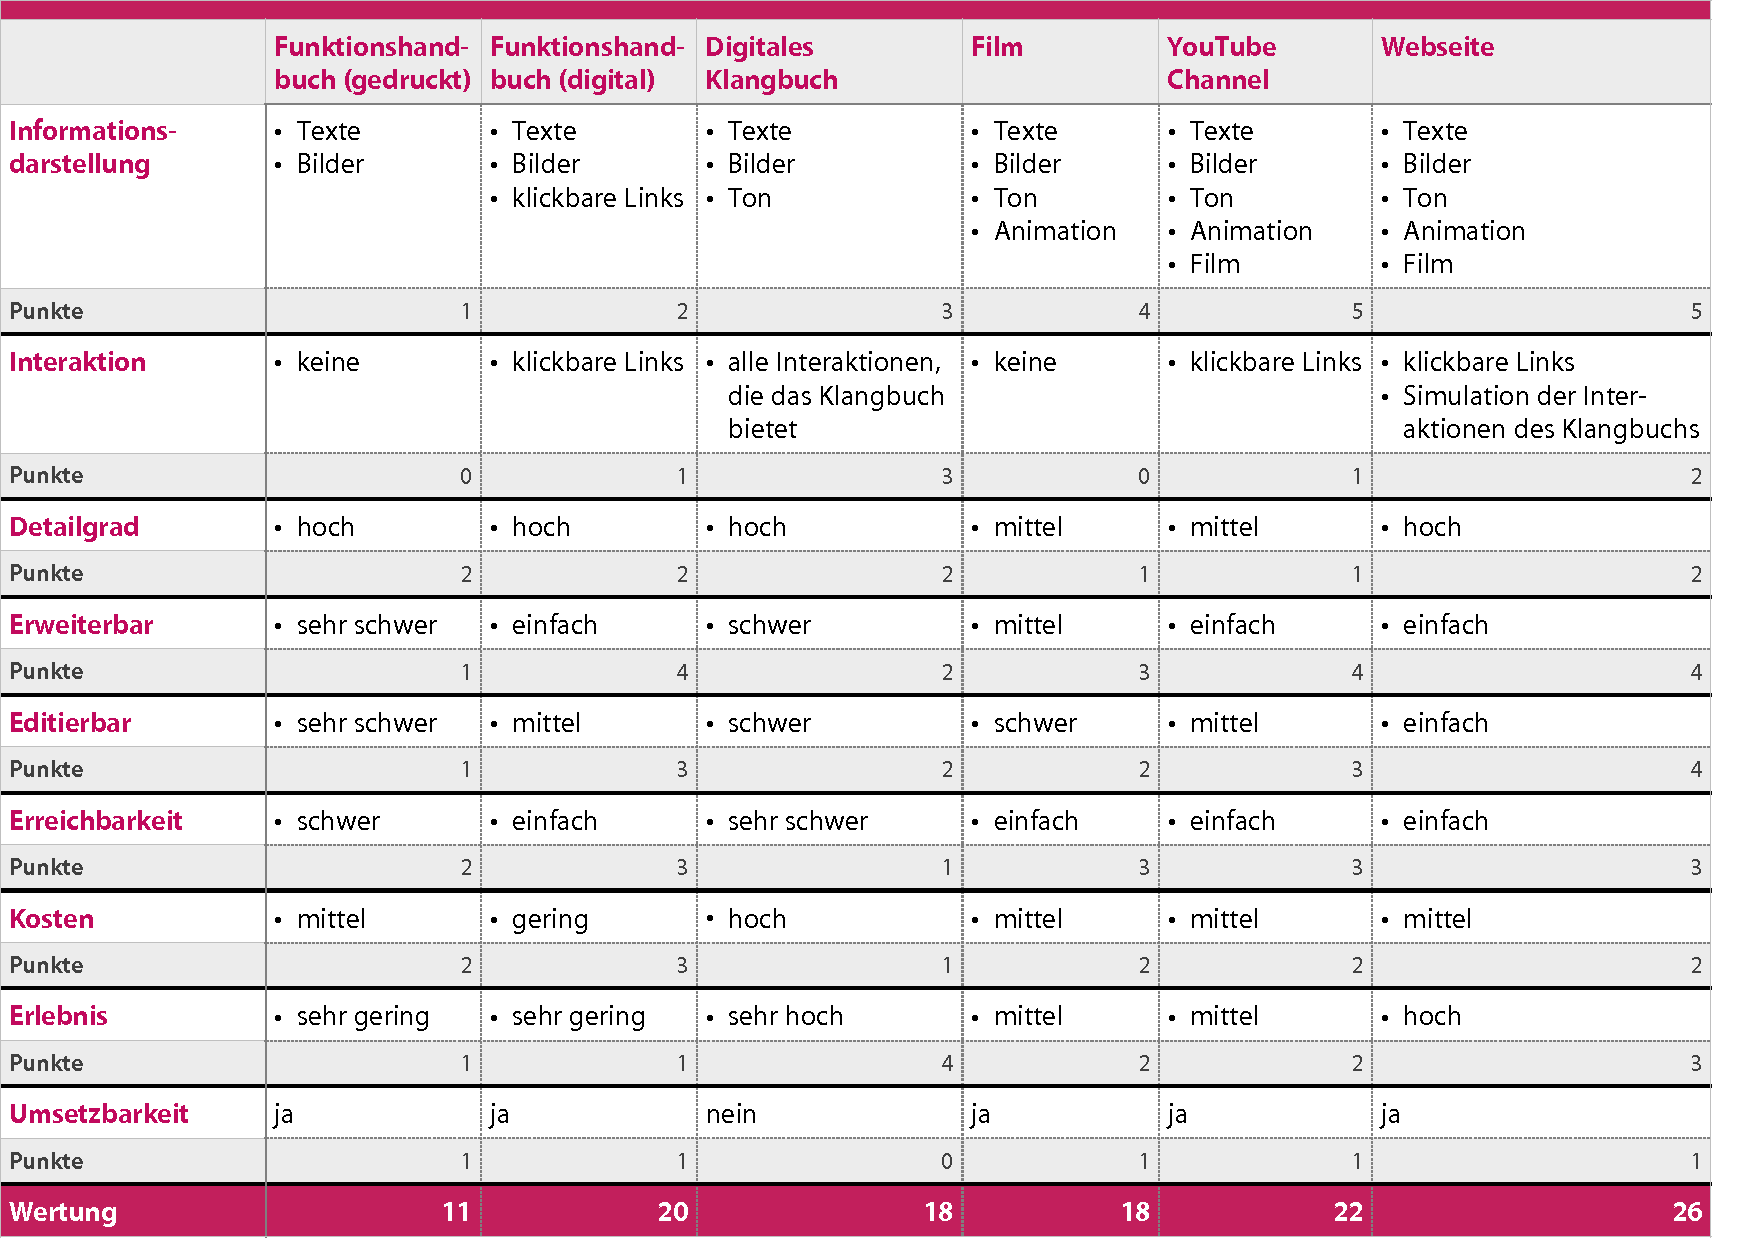
\includegraphics[natwidth=920pt, natheight=95pt, width=1.0\textwidth]{grafiken/leitfaden-bewertung.pdf}
\caption{Bewertungstabelle der möglichen Leitfäden}
\end{figure}


\textbf{Informationsdarstellung}\\
In welcher Form können Informationen zu den Funktionen dargestellt werden?\\
Ein Video-Kanal und eine Website bieten hier alle Möglichkeiten zur Darstellung von Informationen.\\

\textbf{Interaktion}\\
Bietet der Leitfaden dem KlangKünstler eine realistische Interaktion?\\
Der Leitfaden als digitales Klangbuch ist die realste Möglichkeit die Funktionen des digitalen Klangbuchs darzustellen. Dem KlangKünstler werden alle Interaktionen geboten.\\

\textbf{Detailierungsgrad}\\
Wie detailliert lassen sich die Funktionen und Informationen zum digitalen Klangbuch darstellen?\\
Informationen, die zu einer Filmsequenz auf einem Video-Kanal hinterlegt werden können, sind begrenzt.\\


\textbf{Erweiterbarkeit}\\
Lässt sich der Leitfaden problemlos erweitern?\\
Ein digitales Funktionshandbuch, eine Video-Kanal und eine Website lassen sich problemlos erweitern. Ein fertiger Film und ein gedruckter Leitfaden dagegen nicht.\\


\textbf{Editierbarkeit}\\
Lassen sich Informationen im Leitfaden problemlos ändern?\\
Ein digitales Funktionshandbuch, eine Website und die Informationen in einem Video-Kanal lassen sich problemlos ändern. Ein fertiger Film und ein gedruckter Leitfaden dagegen nicht.\\


\textbf{Erreichbarkeit}\\
Ist der Leitfaden für jeden KlangKünstler frei verfügbar / erreichbar?\\
Eine Website und ein Video-Kanal ist für jeden KlangKünstler frei verfügbar. Ein gedruckter Leitfaden muss erst seinen physischen Weg zum KlangKünstler finden.\\


\textbf{Aktualität}\\
Die Aktualität ist nicht in der Tabelle enthalten. Sie bildet sich aus den Kriterien Erweiterbarkeit, Editierbarkeit und Erreichbarkeit. Der Leitfaden ist nur dann so aktuell, wie er auch verändert, ergänzt und erreicht / verteilt werden kann.\\Ein Leitfaden als eigenes Objekt, wie z. B. ein digitales Handbuch (PDF-Datei) oder eine Filmsequenz verlieren ihre Aktualität sobald eine neue Version davon erstellt wurde. Die Anlaufstelle für den KlangKünstler dagegen - in diesem Fall eine Website oder ein Video-Kanal - kann immer den aktuellsten Leitfaden zur Verfügung stellen.\\
Zählt man die vergebenen Punkte der einzelnen Leitfäden für die Kriterien Erweiterbarkeit, Editierbarkeit und Erreichbarkeit zusammen ergibt sich daraus die Bewertung der Aktualität.\\

\textbf{Kosten}\\
Wie hoch sind die Kosten zur Umsetzung des Leitfadens?\\
Die Funktionen müssen für jeden Leitfaden erstellt und beschrieben werden. Ein Handbuch muss jedoch für jeden KlangKünstler gedruckt und versendet werden. Ein digitales Klangbuch als Leitfaden enthält neben Papier auch Technik und die Produktionskosten, die für die Herstellung eines digitalen Klangbuchs notwendig sind. Die Kosten für das Hosting einer Website und das Drehen von Filmsequenzen sind dagegen deutlich geringer.\\

\textbf{Erlebnis}\\
Vermittelt der Leitfaden dem KlangKünstler das besondere Erlebnis des digitalen Klangbuchs?
Nur das Klangbuch selbst kann dem KlangKünstler einen realen Einblick und ein reales Erleben ermöglichen. Durch Webtechnologien ist es möglich die Funktionen des digitalen Klangbuchs auch auf einer Website zu simulieren. In Filmsequenzen lassen sich die Funktionen des digitalen Klangbuchs durch ein Abfilmen des Klangbuchs vermitteln.\\

\textbf{Umsetzbarkeit}\\
Lässt sich der vorgestellte Leitfaden im Rahmen der Bachelorarbeit umsetzen?\\
Das digitale Klangbuch als Leitfaden ist aufgrund der eingesetzten Technik und den damit verbunden Kosten im Rahmen der Bachelorarbeit zu komplex um es zu realisieren. Alle anderen vorgestellten Leitfäden sind umsetzbar.\\


%%%%%%%%%%%%

\subsection{Auswahl Leitfaden}
Die höchste Punktzahl hat der Leitfaden als Website erhalten. Die Vorteile einer Website wurden bereits in "Leitfaden als Website" in Kapitel \ref{VorteileWebsite} genannt. Eine Website bietet den Vorteil, dass sie immer aktuell gehalten und erweitert werden kann. Durch Kombination aus Film, Text und Bildern lässt sich der Leitfaden nicht nur detailliert sondern auch anschaulich darstellen. Der KlangKünstler kann durch das Schauen der Filmsequenzen eine ungefähre Idee des digitalen Klangbuchs erhalten und die Funktionen "miterleben".\\
Im weiteren Verlauf der Arbeit werden die Begriffe "Leitfaden" und "Website" synonym verwendet.\\



%%%%%%%%%%%%%%%%%%%%%%%%%%%%%%%%%%%%%%%%%%%%%%%%%%%%%%%%%%%%%%%%%%%%%%%%%%%%%%%%%%%%%%%%%%%%%%%%
%%%%%%%%%%%%%%%%%%%%%%%%%%%%%%%%%%%%%%%%%%%%%%%%%%%%%%%%%%%%%%%%%%%%%%%%%%%%%%%%%%%%%%%%%%%%%%%%
%%%%%%%%%%%%%%%%%%%%%%%%%%%%%%%%%%%%%%%%%%%%%%%%%%%%%%%%%%%%%%%%%%%%%%%%%%%%%%%%%%%%%%%%%%%%%%%%
%%%%%%%%%%%%%%%%%%%%%%%%%%%%%%%%%%%%%%%%%%%%%%%%%%%%%%%%%%%%%%%%%%%%%%%%%%%%%%%%%%%%%%%%%%%%%%%%
%%%%%%%%%%%%%%%%%%%%%%%%%%%%%%%%%%%%%%%%%%%%%%%%%%%%%%%%%%%%%%%%%%%%%%%%%%%%%%%%%%%%%%%%%%%%%%%%







\chapter{Konzeption Leitfaden}

Im ersten Schritt dieses Kapitels werden die Ziele des Leitfadens definiert. Anschließend wird definiert, wie der Leitfaden idealerweise aufgebaut werden sollte. Im letzten Schritt werden die \gls{videoclip}s konzipiert und Drehbücher dazu erstellt.


%%%%%%%%%%%%
%%%%%%%%%%%%
%%%%%%%%%%%%


\section{Art des Leitfaden}
Der Leitfaden wird als Webseite konzipiert und umgesetzt. Dazu werden Videoclips erstellt und in die Webseite eingebunden. Durch die Kombination aus Videoclips, Text und Bildern lässt sich der Leitfaden nicht nur detailliert sondern auch anschaulich darstellen. 

%%%%%%%%%%%%
%%%%%%%%%%%%
%%%%%%%%%%%%


\section{Vermittlungsziele Leitfaden}
Was soll der Leitfaden vermitteln?

\begin{itemize}
\item Der KlangKünstler soll das Gesamtkonzept "Digitales Klangbuch" verstehen
\item Der KlangKünstler soll den Aufbau des digitalen Klangbuchs verstehen
\item Dem KlangKünstler sollen die Möglichkeiten und Grenzen des digitalen Klangbuchs vermittelt werden
\item Der KlangKünstler soll mögliche Funktionen des digitalen Klangbuchs kennen und verstehen lernen
\item Bei den Besuchern der Website soll Interesse und Begeisterung für das digitale Klangbuch geweckt werden
\item Der KlangKünstler soll inspiriert werden
\end{itemize}


%%%%%%%%%%%%
%%%%%%%%%%%%
%%%%%%%%%%%%

\section{Aufbau Leitfaden}


%%%%%%%%%%%%


\subsection{Einstieg}
Damit der Besucher der Website das digitale Klangbuch kennen und verstehen lernt, soll das digitale Klangbuch erklärt und folgende Fragen beantwortet werden:

\begin{itemize}
\item Was ist das digitale Klangbuch?
\item Was kann man mit dem digitalen Klangbuch machen?
\item Was ist das Besondere an dem digitalen Klangbuch?
\item An wen richtet sich das digitale Klangbuch?
\end{itemize}

Ein kurzes Einführungsvideo, in dem das digitale Klangbuch vorgestellt wird, kann all diese Fragen beantworten. Dieser \gls{videoclip} wird im Folgenden "Startclip" genannt.


%%%%%%%%%%%%


\subsection{Kategorien}
Das digitale Klangbuch bedient mehrere Sinne: den auditiven, visuellen und haptischen Sinn. Da in den Funktionen des Klangbuchs zumeist alle drei Sinne gleichzeitig angesprochen werden, ist eine Unterteilung der Funktionen in die Bereiche Audio, Visuell und Haptik nicht sinnvoll. Jedoch kann im Leitfaden zu jedem dieser Sinne ein Erklärungstext mit Beispielen integriert werden.\\


%%%%%%%%%%%%


\subsection{Auswahl der Klangbuch-Funktionen}
Aufgrund des zeitlich eingeschränkten Rahmens der Bachelorarbeit ist es nicht möglich jede Funktion in einem Video vorzustellen, denn jeder \gls{videoclip} benötigt passendes Audiomaterial, das produziert werden muss. Die Auswahl der Funktionen erfolgte nach folgenden Kriterien:\\

1. Erlebnis / Besonderheit der Funktion\footnote{Erlebnis / Besonderheit im Sinne von: Die vorzustellende Funktion soll ein besonderes Erleben beim Klangkünstler und Hörer hervor rufen und die besonderen Möglichkeiten des digitalen Klangbuchs aufweisen.}\\ 
2. Mindestens eine komplexere Funktion soll umgesetzt werden (z. B. Multitrack)\\
2. Produzierbarkeit des passendes Audiomaterials im Rahmen der Bachelorarbeit\\

Folgende Funktionen wurden ausgewählt:

\begin{itemize}
\item Audio abspielen (Standardfunktion)
\item Multitrack 
\item SongKit
\item Entstehungsgeschichte \gls{song}, im Folgenden "Versions" genannt
\end{itemize}

Weitere Funktionen werden ohne \gls{videoclip} auf der Website vorgestellt. Die haptischen und visuellen Funktionen werden im Einführungsclip vorgestellt.


%%%%%%%%%%%%%%%%%%%%%%%%%%%%%%%%%%%%%%%%%%%%%%%%
%%%%%%%%%%%%%%%%%%%%%%%%%%%%%%%%%%%%%%%%%%%%%%%%
%%%%%%%%%%%%%%%%%%%%%%%%%%%%%%%%%%%%%%%%%%%%%%%%


\section{Konzeption Videoclips}

Für jeden \gls{videoclip} muss ein \gls{song} oder Soundfragment produziert, ein Layout entwickelt und ein Drehbuch inklusive Storyboard erstellt werden. Nach Aufnahme der \gls{videoclip}s werden diese am Rechner montiert und vertont.

\subsection{Produktion Songs / Sounds}
Um die entwickelten, akustischen Funktionsmöglichkeiten in \gls{videoclip}s zu veranschaulichen, wurden passende lizenzfreie \gls{song}s und Soundfragmente benötigt. Diese wurde zum Teil selbst produziert.


\begin{figure}[H]
\centering
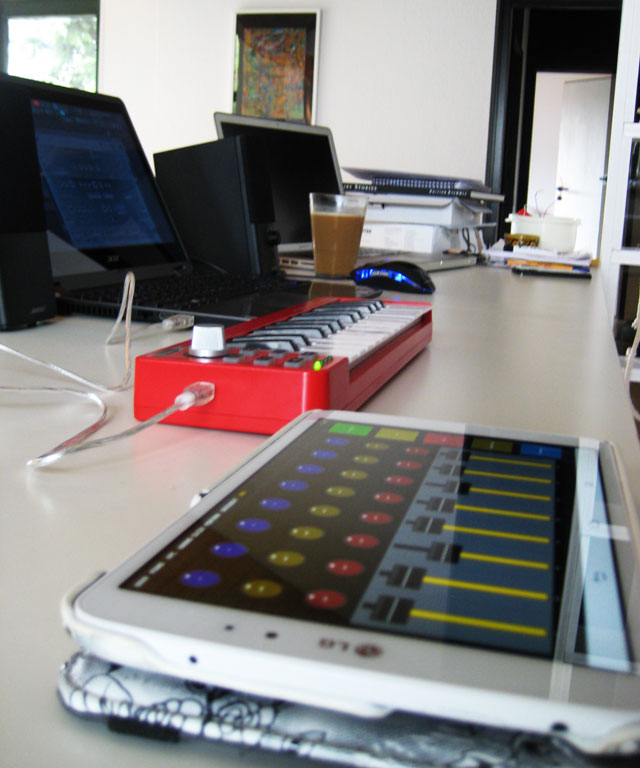
\includegraphics[width=0.5\textwidth]{grafiken/musikproduktion.jpg}
\caption{Produktion der Songs und Soundfragmente}
\end{figure}

Für den \textbf{Start-\gls{clip}} wurde ein \gls{loop} aus der Sound-Bibliothek der Musikproduktions-Software Garageband von Apple ausgewählt und Stimmaufnahmen produziert.\\

Ein \gls{song} mit sieben einzelnen Spuren wurde für den \gls{clip} \textbf{Multitrack} produziert.\\

Für den \gls{clip} \textbf{SongKit} wurden 13 zueinander passende \gls{loop}s produziert. Diese unterteilen sich in Bass, Drums, Melodie, Pad und Effekt.\\

Ein \gls{song} in fünf Versionen wurde für den \gls{clip} \textbf{Versions} produziert: Skizze-, Probe-\\raum-, Studio-, Akustik- und Live-Version. 


%%%%%%%%%%%%
%%%%%%%%%%%%


\subsection{Design \& Layouts}\label{design}
Für den Leitfaden wurde ein Design entwickelt, welches Schriften, Farben und das Logo beinhaltet. Anhand dieser Vorgaben wurden die Layouts für die ausgewählten Funktionen entwickelt. Die Grafiken in den Layouts wurden größtenteils selbst erstellt, einige stammen von der lizenzfreien Bildbörse Pixabay\footnote{Lizenzfreie Bildbörse Pixabay, die verwendeten Bilder benötigen keinen Bildnachweis: \url{https://pixabay.com}}.

\begin{figure}[H]
\centering
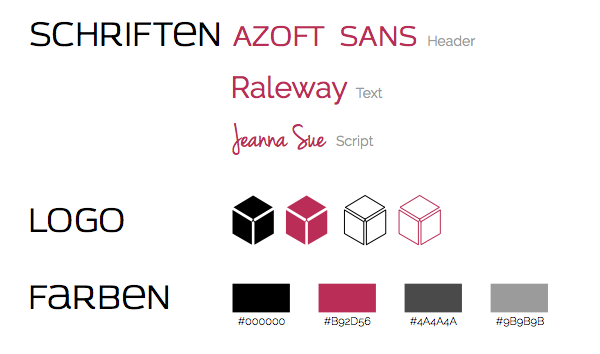
\includegraphics[width=0.7\textwidth]{grafiken/corporatedesign1.png}
\caption{Design: Schriften, Farben und Logo}
\label{fig:design}
\end{figure}

\subsubsection{Logo}
Bei der Entwicklung des Logos wurden wichtige und interessante Merkmale des digitalen Klangbuchs ermittelt:
\begin{itemize}
\item drei Sinne: Hör-, Seh-, Tastsinn
\item alle Sinne werden zugleich angesprochen
\item berührungsempfindliche Elemente
\item das Buch enthält technische Komponenten
\item Erlebnis
\end{itemize}

Anhand der Merkmale wurde ein Logo entwickelt; nicht jedes Merkmal konnte in dem Logo wieder gespiegelt werden:\\
Die drei Sinne können durch drei Teile symbolisiert werden. Da alle Sinne gleichzeitig angesprochen werden, sollten alle Teile miteinander verbunden werden. Das Logo kann so gestaltet werden, dass es an einen \gls{button} erinnert. So kann die Berührungsempfindlichkeit des Buches im Logo dargestellt werden. Klare Linien unterstreichen die technische Ausrichtung des Buches.

\begin{figure}[H]
\centering

\includegraphics[width=0.7\textwidth]{grafiken/logo.png}
\caption{Design: Schriften, Farben und Logo}
\label{fig:logo}
\end{figure}

Das entwickelte Logo kann in den Farben (s. Farbwerte in Abbildung \ref{fig:design}) Pink oder Schwarz dargestellt werden. Es kann zudem gefüllt oder nur aus Außenlinien bestehen.\\
Das Logo dient in den Layouts grundsätzlich als \gls{button} um eine Audiodatei zu starten oder zu stoppen.

%%%%%%%%%%%%
%%%%%%%%%%%%


\subsection{Digitales Klangbuch}

Die \gls{videoclip}s sollen dem KlangKünstler das digitale Klangbuch näher bringen. Dazu ist es sinnvoll das digitale Klangbuch in den Videos zu präsentieren. Dazu wurde ein nichtfunktionaler Prototyp erstellt.\\

\begin{figure}[H]
\centering

\includegraphics[width=0.8\textwidth]{grafiken/cutting.png}
\caption{Die gedruckten Layouts wurden mit einem Cutter-Messer ausgeschnitten und in ein Buch geklebt}
\end{figure}


Ein großformatiges Buch dient dazu als Basis. Für jeden \gls{videoclip} wurde ein Layout entwickelt, gedruckt und in das Buch montiert. Ein Audioeingang für den Kopfhörer wurde ebenfalls in das Buch integriert.\\


\begin{figure}[H]
\centering
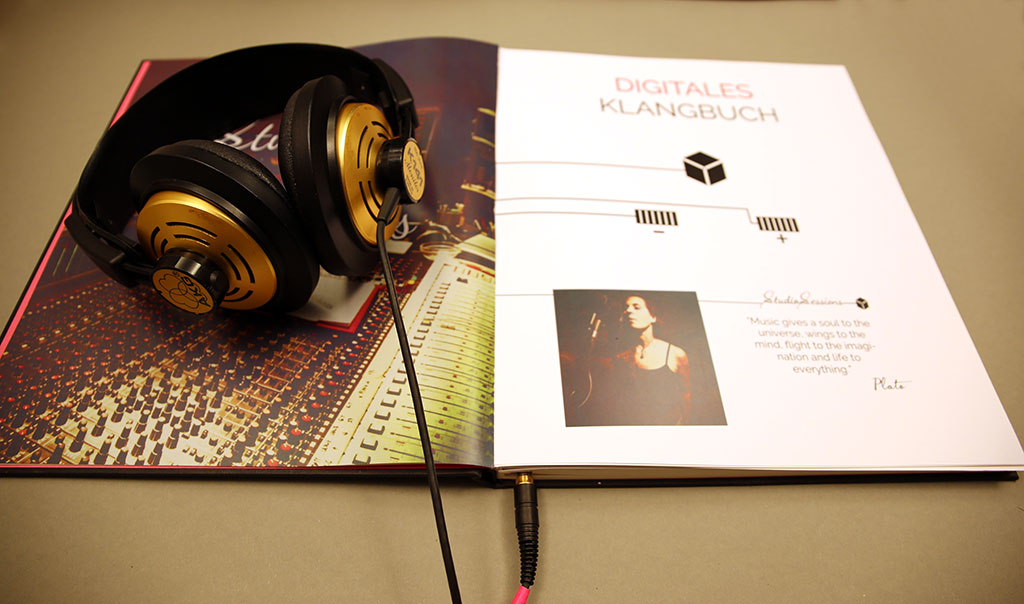
\includegraphics[width=0.9\textwidth]{grafiken/gebautes_klangbuch.jpg}
\caption{Prototyp des digitalen Klangbuchs}
\end{figure}

%%%%%%%%%%%%
%%%%%%%%%%%%




\subsection{Konzeption Intro \& Outro}
Jeder \gls{videoclip} wird ähnliche aufgebaut. Der Vorteil daran ist, dass die Videoclips so einen Wiedererkennungseffekt und ein konsistentes, professionelles Erscheinungsbild haben.\\


\textbf{\gls{intro}}\\
Der Name des Videoclips oder der Funktion, die in dem Videoclip vorgestellt wird, soll eingeblendet werden.
Darunter das Logo des Digitalen Klangbuchs. Folgendes Material wird benötigt:

\begin{itemize}
\item digitales Klangbuch
\item Kopfhöreranschluss
\item Kopfhörer
\item evtl. \gls{loop}
\end{itemize}

\vspace{0.5cm}

Folgendes \gls{intro}-Layout wurde entwickelt:

\begin{figure}[H]
\centering

\includegraphics[width=1.0\textwidth]{grafiken/layoutintro.png}
\caption{Layout des \gls{intro}s für die Funktion Multitrack}
\end{figure}


\textbf{\gls{outro}}\\
Der Schriftzug "Digitales Klangbuch" mit dem Logo, ein Hinweis auf die Website und die Urheberrechte sollen integriert werden.\\

Folgendes \gls{outro}-Layout wurde entwickelt:

\begin{figure}[H]
\centering
\frame{
\includegraphics[width=0.8\textwidth]{grafiken/layoutoutro.png}}
\caption{Layout des \gls{outro}s}
\end{figure}


%%%%%%%%%%%%
%%%%%%%%%%%%

\subsection{Konzeption "Startclip"}
Der Startclip wird als Einführungsvideo auf der Startseite der Website eingebunden. Dem Besucher der Seite soll damit das Buch im Allgemeinen erklärt werden. Dazu wird ein \gls{button} zum Starten und Stoppen des Klangs, eine Lautstärkeregelung und Bilder und Texte integriert. Da der Startclip keine einzelne Funktion vorführt, sondern das Buch an sich präsentiert, wird hier nicht das zuvor entwickelte \gls{intro}, sondern ein eigenes integriert. Dieses hat den folgenden Ablauf:

\begin{itemize}
\item Aufnahme des geschlossenen Buches mit beiliegenden Kopfhörern
\item Kopfhörer werden aufgesetzt
\item der Kopfhörer wird an das Buch angeschlossen
\item das Buch wird aufgeblättert
\end{itemize}


\textbf{Material für den Videoclip}
\begin{itemize}
\item Klangbuch
\item Kopfhörer
\item doppelseitiges Layout mit Bildern, Texten, Lautstärkeregelung, Start\gls{button}
\item Song I (ca. 20 Sekunden)
\item 2. Layout nach Umblättern (z. B. Layout von Multitrack)
\item Song II (ca. 10 Sekunden) (z. B. Song von Multitrack)
\end{itemize}

\vspace{0.5cm}



\textbf{Layout "Startclip"}\\
Das doppelseitige Layout enthält Bilder, Texte und Interaktionsschaltflächen. Die linke Seite zeigt ein Druckbeispiel für ein Foto und einen Titel. Auf der rechten Seite gibt es eine Schaltfläche zum Starten und Stoppen des \gls{song}s und \gls{button}s zur Regelung der Lautstärke. Es ist ebenfalls ein Foto und ein Text abgedruckt. Dazu gibt es einen weiteren \gls{button}, der mit einer Überschrift verbunden ist "Studio Sessions".Jedes berührungsempfindliche Element ist mit einer schwarzen Linie mit dem Buchrücken verbunden. Die Linien berühren sich nicht. Die Linien wurden bewusst so platziert, dass sie kaum versehentlich berührt werden können.


\begin{figure}[H]
\centering
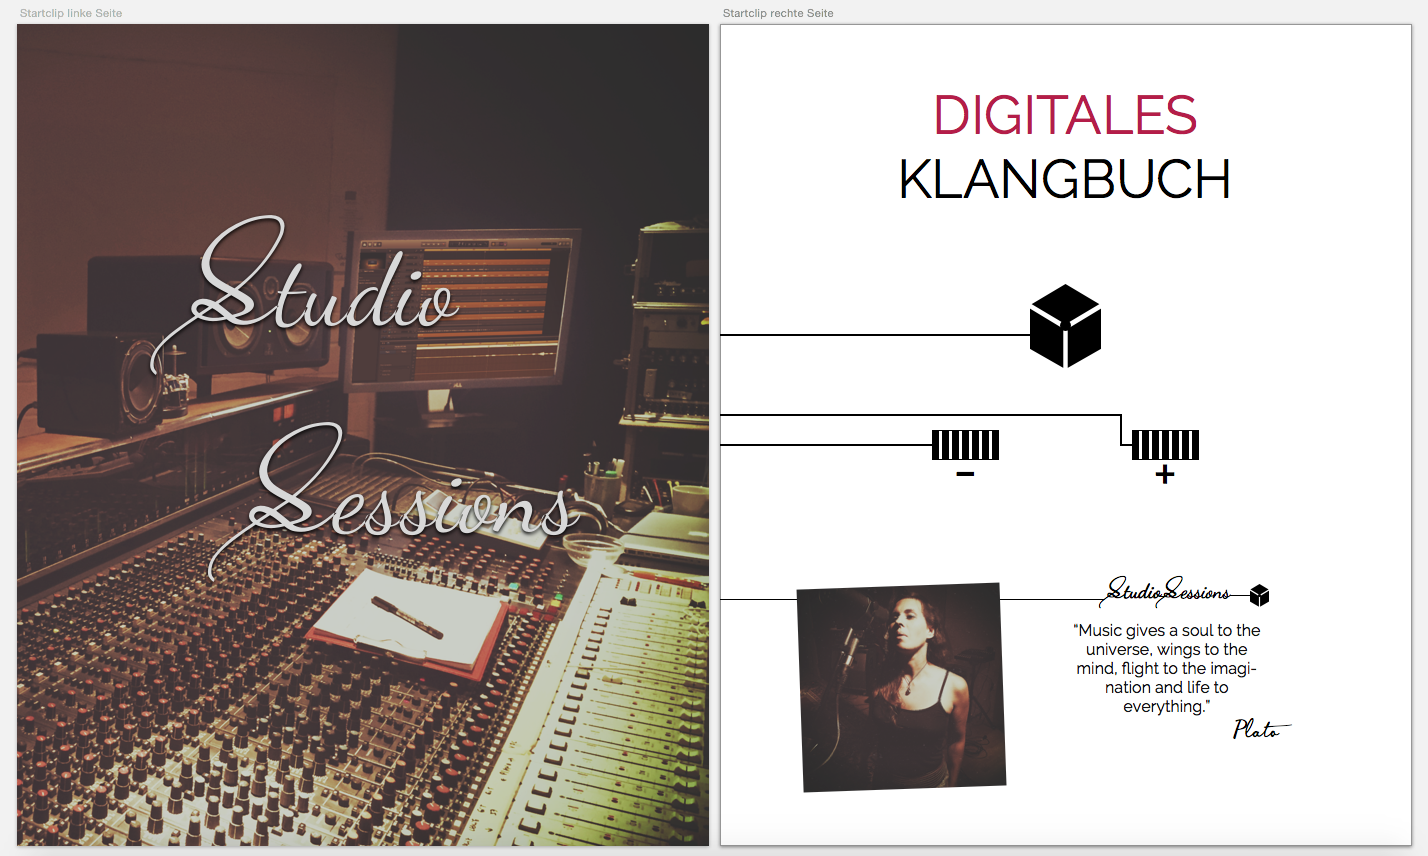
\includegraphics[width=1.0\textwidth]{grafiken/startclip.png}
\caption{Layout für den Startclip. Links: Printbeispiel, Hintergrundfoto mit Titel\\Rechts: Interaktionsmöglichkeiten: Start-/Stopp \gls{button} für den \gls{song}, Lautstärkeregelung, Start-/Stopbutton zum Text}
\label{fig:startclip}
\end{figure}


\vspace{0.5cm}





%%%%%%%%%%%%
%%%%%%%%%%%%
%%%%%%%%%%%%



\subsection{Konzeption "Multitrack"}
Für die Funktion Multitrack wurde der \gls{song} "Sunday Sessions" mit 7 einzelnen Spuren produziert. Im Video soll die Mehrspur-Funktion veranschaulicht werden, in dem einzelne Spuren stumm und wieder angeschaltet werden. Auch die Lautstärke soll sich regeln lassen.\\

Das Layout für die Funktion Multitrack soll auf das Wesentliche, die berührungsempfindlichen Elemente, reduziert sein. Hier liegt der Fokus auf die Interaktionsmöglichkeiten, die die Funktion bietet. Um die aktivierten Spuren kenntlich zu machen, bietet es sich an, diese mit SMD-LEDs zu versehen. Da das digitale Klangbuch ein nichtfunktionaler Prototyp ist, müsste das Leuchten der SMD-LEDs in der Filmmontage simuliert werden. Aus zeitlichen Gründen wurde die Idee der integrierten SMD-LEDs verworfen.\\

Ziel des Clips ist es dem KlangKünstler die Möglichkeit zur Einbindung einer interaktiven Mehrspur-Funktion zu vermitteln.\\


\textbf{Material für den Videoclip}
\begin{itemize}
\item Klangbuch
\item Kopfhörer
\item Layout mit 7 Spuren, Lautstärkeregelung, Startbutton, \gls{button} um alle Spuren aus zustellen.
\item Song mit 7 Spuren
\item Story
\end{itemize}

\vspace{0.5cm}



\textbf{Layout "Multitrack"}\\
Das Layout ist auf das Wesentliche, die berührungsempfindlichen Elemente, reduziert. Es gibt eine Schaltfläche zum Starten und Stoppen des \gls{song}s (\gls{button} neben "Sunday Sessions") und eine zum Stummschalten aller Spuren (\gls{button} neben "Off All"). Die Spuren sind breit gestaltet und beschriftet. Neben jeder Spur befinden Elemente zur Lautstärkeregelung. Jedes berührungsempfindliche Element ist mit einer schwarzen Linie mit dem Buchrücken verbunden. Die Linien berühren sich nicht. Die Linien wurden bewusst so platziert, dass sie kaum versehentlich berührt werden können.

\begin{figure}[H]
\centering
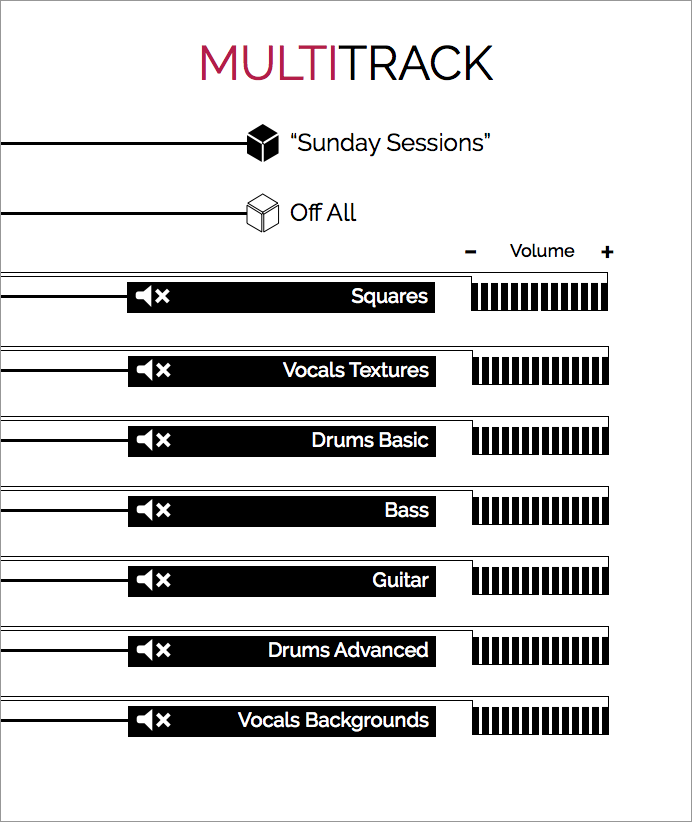
\includegraphics[width=0.6\textwidth]{grafiken/multitrack.png}
\caption{Layout für die Funktion Multitrack.}
\end{figure}

\vspace{0.5cm}




%%%%%%%%%%%%


\subsection{Konzeption "SongKit"}
Für die Funktion SongKit wurde der \gls{loop} "Monday Sessions" mit fünf Spuren und jeweils fünf Variationen erstellt. Im Video soll der Nutzer den \gls{loop} verändern, in dem er auf die verschiedenen Variationen der fünf Spuren klickt.\\

Das Layout für die Funktion SongKit soll auf das Wesentliche, die berührungsempfindlichen Elemente, reduziert sein. Hier liegt der Fokus auf die Interaktionsmöglichkeiten, die die Funktion bietet. Um die Spuren voneinander zu unterscheiden zu können, soll jede Spur mit eigenen Symbolen ausgestattet werden. Um die aktivierten \gls{loop}s kenntlich zu machen, bietet es sich an die Spuren mit SMD-LEDs zu versehen. Da das digitale Klangbuch ein nichtfunktionaler Prototyp ist, müsste das Leuchten der SMD-LEDs in der Filmmontage simuliert werden. Aus zeitlichen Gründen wurde die Idee der integrierten SMD-LEDs jedoch verworfen.\\

Ziel des Clips ist es dem KlangKünstler die Funktion SongKit zu vermitteln und ihn zu neuen Ideen zu inspirieren. Die Funktion SongKit eignet sich z. B. dafür, um unveröffentlichtes, unvollendetes Material dem Fan zur Verfügung zu stellen.\\


\textbf{Material für den Videoclip}
\begin{itemize}
\item Klangbuch
\item Kopfhörer
\item Layout mit fünf Spuren zu je fünf Variationen + Startbutton
\item \gls{loop} mit fünf Spuren zu mind. drei Variationen (es müssen nicht alle Variationen im Videoclip angesteuert werden)
\item Story
\end{itemize}

\vspace{0.5cm}



\textbf{Layout "SongKit"}\\
Das Layout ist auf das Wesentliche, die berührungsempfindlichen Elemente, reduziert. Es gibt eine Schaltfläche zum Starten und Stoppen des \gls{song}s (\gls{button} neben "Monday Sessions"). Jede Spur enthält fünf \gls{loop}s, die mit einem Symbol dargestellt werden. Jede Spur hat dabei ein eigenes Symbol. Jedes berührungsempfindliche Element ist mit einer schwarzen Linie mit dem Buchrücken verbunden. Die Linien berühren sich nicht. Die Linien wurden bewusst so platziert, dass sie kaum versehentlich berührt werden können.

\begin{figure}[H]
\centering

\includegraphics[width=0.6\textwidth]{grafiken/songkit.png}
\caption{Layout für die Funktion SongKit.}
\end{figure}

\vspace{0.5cm}


%%%%%%%%%%%%


\subsection{Konzeption "Versions"}
Für die Funktion Versions wurde der \gls{song} "We are here" in vier Versionen produziert: Als Skizze, eine Proberaumversion, eine Studioversion und eine Aufnahme von einem Live-Auftritt. Zusätzlich dazu wurde noch eine Akustik-Version erstellt. Diese vier Versionen (+ Akustik Version), die der \gls{song} durchläuft, sollen im Videoclip vorgestellt werden.\\ 

Das Layout für die Funktion Versions soll vor allem ein Beispiel zu den visuellen Darstellungsmöglichkeiten im Klangbuch sein: Darstellung von Bildern, Informationen, Songtexten, etc.\\

Ziel des Clips ist es dem KlangKünstler zum Einen die Funktion Versions zu vermitteln. Ihm sollen aber auch die Möglichkeiten zur Darstellung von grafischem und textuellen Inhalten Nahe gebracht werden. Er soll dazu inspiriert werden mehr über sich und die Musik zu erzählen. Material, was bisher auf einer Website, in einem \gls{artwork} oder \gls{booklet} platziert wurde oder unveröffentlicht blieb, hat mehr Raum im digitalen Klangbuch.\\


\textbf{Material für den Videoclip}
\begin{itemize}
\item Klangbuch
\item Kopfhörer
\item vier doppelseitige Layouts mit Startbutton + Fotos + Text
\item Song in vier Versionen + Akustik Version
\item Story
\end{itemize}

\vspace{0.5cm}



\textbf{Layout "Versions"}\\
Für die Visualisierung der Funktion Versions wurde zu jeder \gls{song}-Version ein doppelseitiges Layout erstellt. Die linke Seite ist vollflächig mit einem Bild, passend zur vorgestellten \gls{song}-Version, gefüllt. Die Seite ist jeweils mit dem Namen des \gls{song}s "We are here" und der Version des \gls{song}s betitelt, z. B. Proberaum. Die linke Seite enthält je einen \gls{button} zum Starten und Stoppen des \gls{song}s. Der Titel des \gls{song}s und der \gls{song}-Version werden ebenfalls aufgeführt. Die Seiten sind außerdem mit passenden Bildern und Blindtexten gefüllt. Jedes berührungsempfindliche Element ist mit einer schwarzen Linie mit dem Buchrücken verbunden. Die Linien berühren sich nicht. Die Linien wurden bewusst so platziert, dass sie nicht versehentlich berührt werden können.

\begin{figure}[H]
\centering
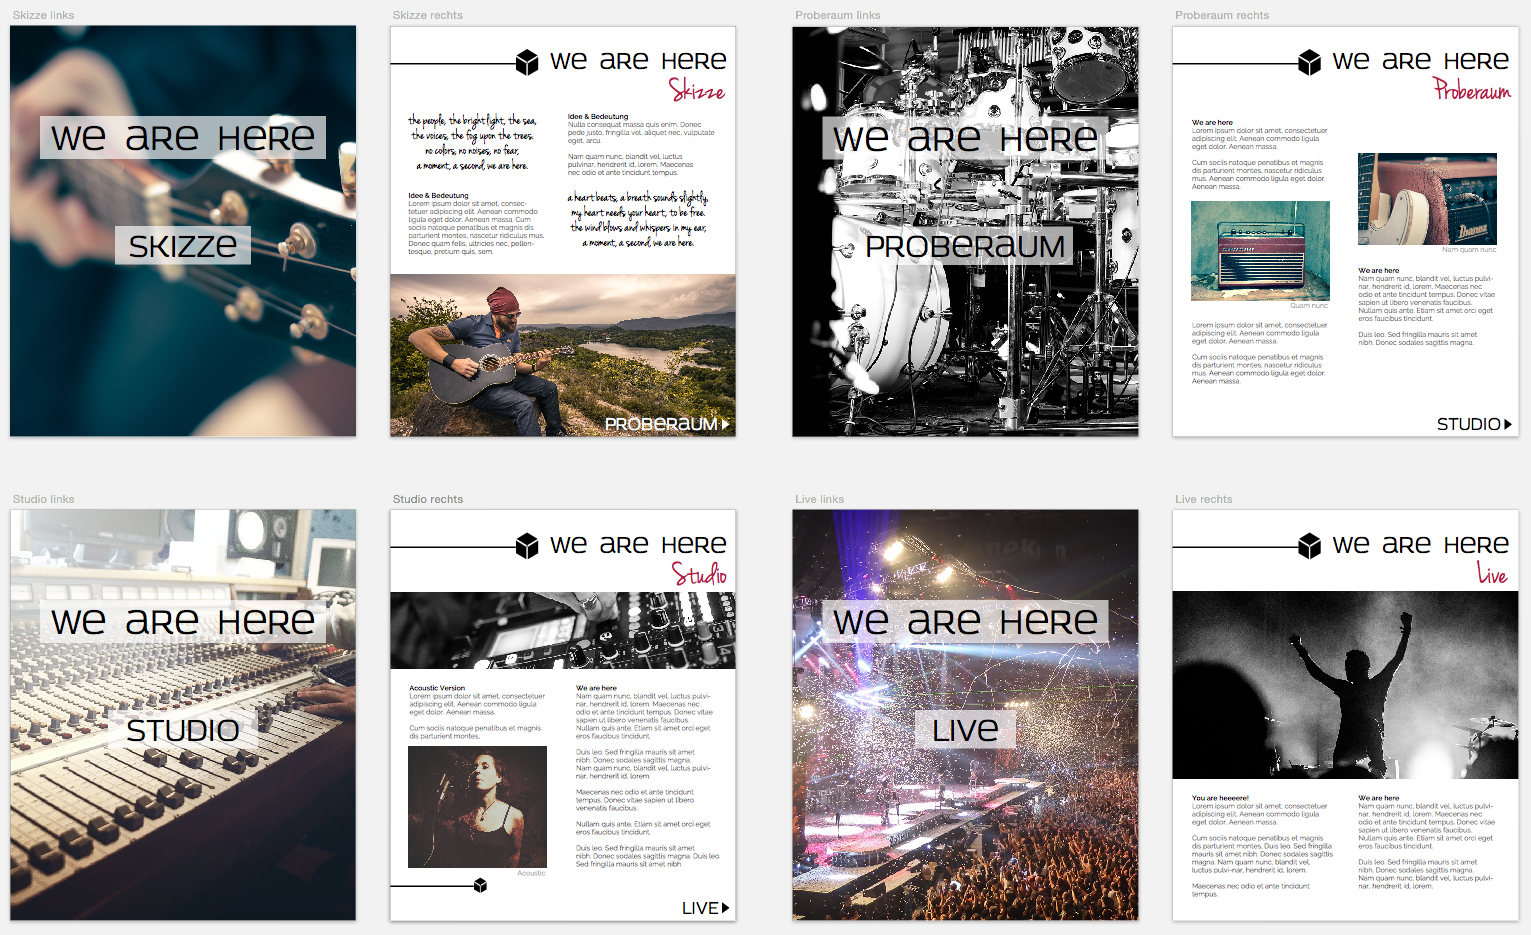
\includegraphics[width=1.0\textwidth]{grafiken/songversions.png}
\caption{}
\end{figure}

\vspace{0.5cm}


%%%%%%%%%%%%



\subsection{Story \& Storyboards}
Für jeden Videoclip wurde eine Story erstellt, die im Anhang einsehbar ist. Für die Visualisierung der Funktionen Multitrack und SongKit wurde zuvor der akustische Ablauf (Reihenfolge des Starten und Stoppens der einzelnen Spuren) in einer Musikproduktionssoftware getestet. Auf ein Storyboard wurde verzichtet, da sich die Kameraeinstellung nicht ändert. Das Buch wird einmal im geschlossenen und im geöffneten Zustand, mit dem jeweils dafür erstellten Layout, für ca. 10 Sekunden aufgenommen. Die auszuführenden Aktionen (Kopfhörer einstecken, Buch aufblättern, Schaltfläche berühren, etc.) erfolgen sequenziell. Alle Funktionen werden von einer Hand ausgeführt. Initial ruht die Hand außerhalb des sichtbaren Bereichs. Bei Ausführung der jeweiligen Funktion  wird die Hand sichtbar und geht nach Ausführung wieder in den nicht sichtbaren Bereich zurück.


\vspace{0.5cm}



%%%%%%%%%%%%%%%%%%%%%%%%%%%%%%%%%%%%
%%%%%%%%%%%%%%%%%%%%%%%%%%%%%%%%%%%%

\section{Webhosting \& Domain}
Um die Website ins verfügbar zu machen, wird ein strategisch sinnvoller Domainname benötigt. Der Domainname soll nah an dem Produkt "Digitales Klangbuch" sein und möglichst kurz, prägnant und verfügbar sein. Folgende Namen wurden auf Verfügbarkeit geprüft:

\begin{itemize}
\item klangbuch.de (belegt, unkonfiguriert)
\item klangbuch.com (belegt, bei Aufruf Fehlermeldung, nicht erreichbar)
\item klangbuch.net (frei)
\item digitales-klangbuch.de (frei)
\item digitales-klangbuch.com (frei)
\item digitales-klangbuch.net (frei)
\end{itemize}

Die Wahl fiel auf die Domain "klangbuch.net", da die verkürzte Version (klangbuch statt digitales-klangbuch) einprägsamer ist. 


%%%%%%%%%%%%%%%%%%%%%%%%%%%%%%%%%%%%
%%%%%%%%%%%%%%%%%%%%%%%%%%%%%%%%%%%%

\section{Konzeption Website}
Um die Realisierbarkeit innerhalb des zeitlichen Rahmens der Bachelorarbeit sicher zu stellen, soll die erste Version des Leitfadens als Website nur die wichtigsten Inhalte abbilden:

\begin{itemize}
\item Einbinden aller erstellten \gls{videoclip}s
\item Erklärungstext zu den erstellten \gls{videoclip}s
\item kurzer Einleitungstext zum digitalen Klangbuch
\end{itemize}

Die Website soll dem Besucher direkt einen Einstieg in das digitale Klangbuch geben. Daher ist es sinnvoll den Startclip als ersten \gls{clip} einzubinden. Das entwickelte Design (s. Kapitel \ref{design}) wird ebenfalls für die Website verwendet. Die Website soll ein reduziertes Design haben, zum digitalen Klangbuch passen und ein reaktionsfähiges\footnote{Reaktionsfähig oder Responsive ist ein Ausdruck aus der Webentwicklung. \gls{responsive} Webdesign bedeutet, dass sich das Layout einer Website auf unterschiedlichen Endgeräten anpasst.} Layout haben. Um den Aufwand der Entwicklung und des Testings möglichst gering zu halten, wurde hierbei die Nutzung eines fertigen Template-Sets in Erwägung gezogen. Für den Fall, dass kein passendes Template gefunden wird, muss eine eigene Entwicklung erfolgen.\\

\textbf{Sprache}\\
Die Website wird komplett in englischer Sprache sein. Dies hat den Vorteil, dass die Website einem internationalen Publikum präsentiert werden kann. Der Begriff "Digitales Klangbuch" bleibt dabei in deutscher Sprache, da dies der Name des Projekts ist.\\

\textbf{Ideenbuch als Titel}\\
Der Leitfaden wird auf der Website selbst als Ideenbuch betitelt. Die im Leitfaden vorgestellten Funktionen sind Ideen, die den KlangKünstler dazu inspirieren sollen, eigene Ideen zu entwickeln. Daher passt der Titel "Ideenbuch" besser, als der Titel "Leitfaden".


%%%%%%%%%%%%%%%%%%%%%%%%%%%%%%%%%%%%
%%%%%%%%%%%%%%%%%%%%%%%%%%%%%%%%%%%%
%%%%%%%%%%%%%%%%%%%%%%%%%%%%%%%%%%%%
%%%%%%%%%%%%%%%%%%%%%%%%%%%%%%%%%%%%
%%%%%%%%%%%%%%%%%%%%%%%%%%%%%%%%%%%%
%%%%%%%%%%%%%%%%%%%%%%%%%%%%%%%%%%%%







\chapter{Umsetzung Leitfaden}
Um den Leitfaden als Website umzusetzen, muss ein geeignetes Template-Set recherchiert und an das entwickelte Design angepasst werden. Wird kein passendes Template-Set gefunden, wird selbst eines entwickelt. Die \gls{videoclip}s müssen gedreht, montiert, in ein internettaugliches Format konvertiert und in die Website eingebunden werden. Es müssen Informations- und Erklärungstexte in englischer Sprache verfasst werden. Die Website muss auf verschiedenen Browsern und Endgeräten getestet werden.


%%%%%%%%%%%%%%%%%%%%%%%%%%%%%%%%%%%%
%%%%%%%%%%%%%%%%%%%%%%%%%%%%%%%%%%%%

\section{Videodreh \& Montage}

\subsection{Videodreh}

\textbf{Kameraperspektive}\\
Die Videoclips sollen das digitale Klangbuch und die Interaktion mit dem Buch zeigen. Damit der Zuschauer sich auf das Wesentliche, das digitale Klangbuch und die vorgestellte Funktion, konzentrieren kann, ist es sinnvoll das Buch aus der Vogelperspektive oder der Aufsicht zu filmen und einen neutralen Hintergrund zu wählen. Es sollen nur die Hände des Nutzers in dem Film, der die Interaktionen durchführt, über das Buch gleitet und Elemente berührt, zu sehen sein.\\

Es wurden Testaufnahmen zur Aufsicht und zur Vogelperspektive gemacht. Die Wahl fiel auf die Kameraperspektive Aufsicht, da diese dem Zuschauer das Gefühl vermittelt, aus seinen Augen auf das Buch zu schauen und es selbst zu benutzen.

\begin{figure}[H]
\centering
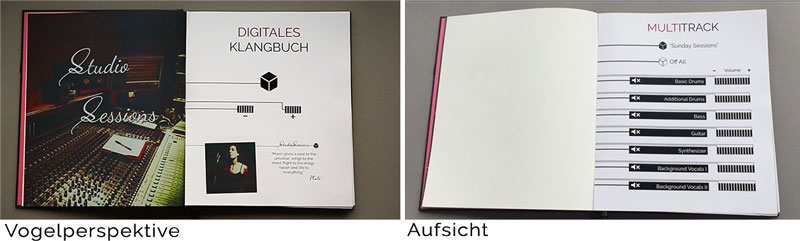
\includegraphics[width=0.8\textwidth]{grafiken/perspektive.jpg}
\caption{Kameraperspektive; Links: Vogelperspektive; Rechts: Aufsicht, vermittelt den Eindruck aus den eigenen Augen auf das Buch zu schauen}
\end{figure}



\textbf{Ausleuchtung, Kameraauswahl \& Probleme}\\
Das zu filmende Buch besteht aus glänzenden, voll- und teil-bedruckten Seiten. Um Reflexionen zu vermeiden, soll das Buch daher nicht direkt, sondern indirekt beleuchtet werden. Auch Schatten, die durch die Bewegung der Hände entstehen, sollen möglichst gering sein.\\

Im ersten Schritt wurde eine DSLR-Kamera für die Aufnahmen der \gls{clip}s verwendet. In einem dunklen Raum mit weißen Wänden und weißer Decke wurde ein Setup mit künstlichem Licht aufgebaut. Es wurden Testaufnahmen zu unterschiedlichen Beleuchtungssituationen gemacht. Trotz indirektem Licht konnten Reflexionen nicht vermieden werden. Durch den hohen Weißanteil auf den Buchseiten wurden die Kanten der Texte im Buch unscharf. Ebenfalls gab es Probleme mit der Farbdarstellung des Buchcovers. Der Druck ist leicht glänzend und schwarz mit pinker Schrift. Die Farbe Schwarz konnte, trotz manuellen Weißabgleichs, nicht ausreichend farbintensiv aufgenommen werden. Durch Einsatz eines Polarisationsfilters, der Licht einer bestimmten Polarisationsrichtung heraus filtert, hätten die Reflexionen absorbiert werden können. Dieser Filter konnte jedoch nicht zum Zeitpunkt der Arbeit beschafft werden.\\
Das Setup wurde dann in einen Raum mit großen Fenstern und natürlichem Licht aufgebaut. Durch das natürliche Licht entstanden deutlich weniger Reflexionen. Jedoch gab es weiterhin Probleme mit unscharfen Kanten und nicht korrekten Farbdarstellungen.\\
Als zweites wurde ein iPhone 6 zur Aufnahme der \gls{clip}s verwendet. Durch die Aufnahme mit dem iPhone 6 und natürlichem Licht, konnten Reflexionen, unscharfe Kanten und Probleme bei der Farbdarstellung signifikant reduziert werden.



\begin{figure}[H]
\centering
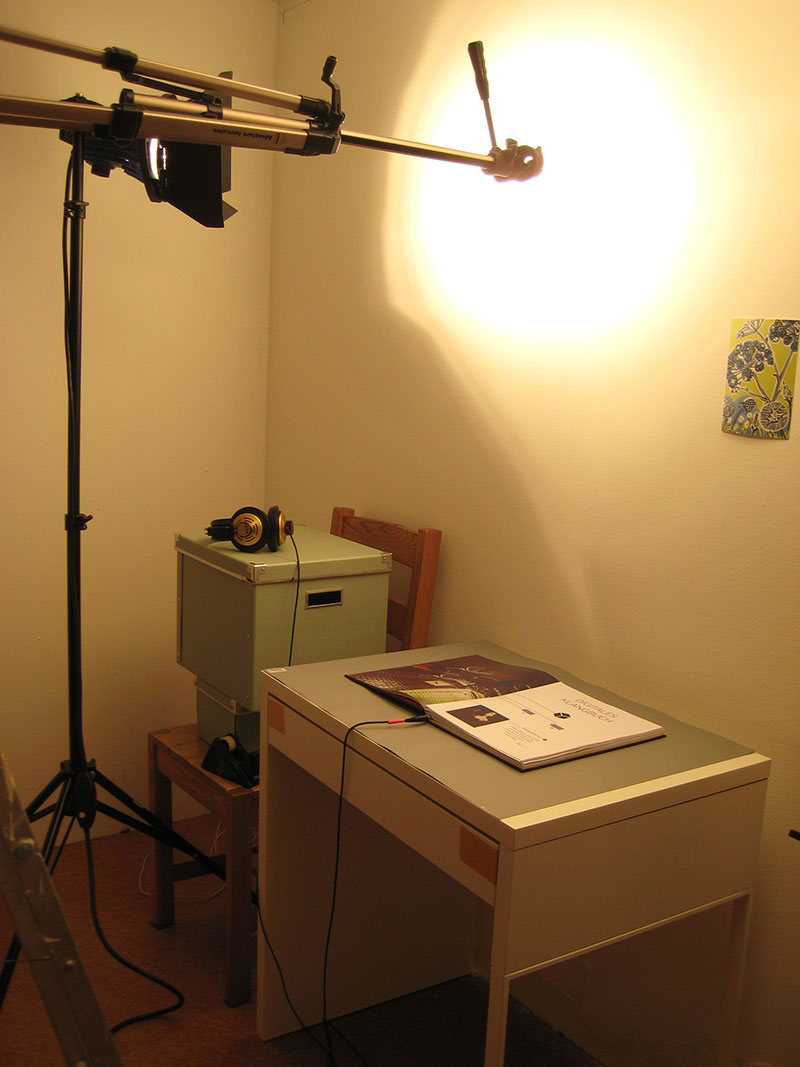
\includegraphics[width=0.3\textwidth]{grafiken/testaufnahmen.jpg}
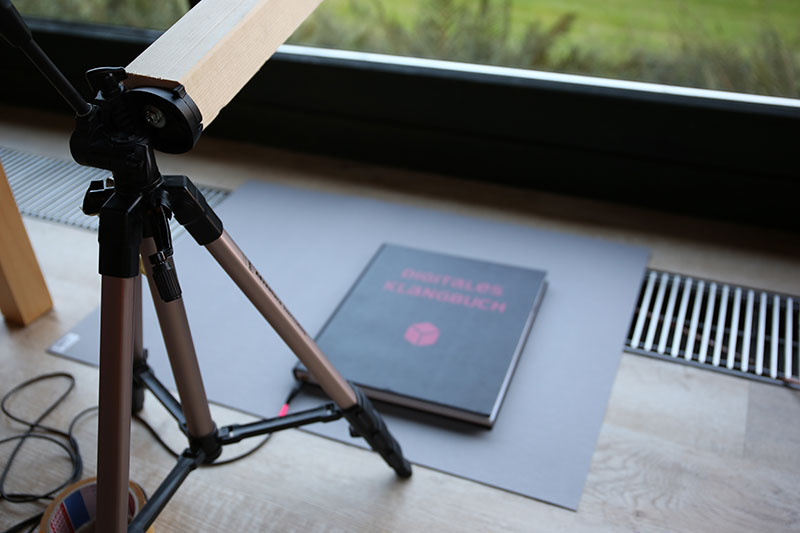
\includegraphics[width=0.4\textwidth]{grafiken/setupII.jpg}
\caption{Setup Testaufnahmen; Links: Künstliches Licht; Rechts: Natürliches Licht}
\end{figure}



\subsection{Montage der \gls{clip}s}
Im Anschluss an den Dreh wurden die einzelnen \gls{clip}s vertont und montiert. Hier bestand die Möglichkeit die Informationen zu den einzelnen \gls{clip}s im Video textuell, z. B. durch eine Bauchbinde, einzublenden oder durch die Aufnahme einer Tonspur zu integrieren. Da in den \gls{clip}s die Interaktion mit Musik dargestellt wird, würde eine weitere Tonspur (Stimme, die die Funktion in dem \gls{clip} erklärt), zu sehr davon ablenken. Der Zuschauer soll sich auf die Veränderungen der Musik konzentrieren, diese sollte nicht durch eine weitere Tonspur belegt werden. Im schlechtesten Fall würde die Tonspur in der Musik untergehen. Daher fiel die Wahl auf das Einblenden von Texten im Video. Um die Konsistenz in allen \gls{clip}s zu bewahren, wird eine Bauchbinde eingesetzt. Diese kann in jedem \gls{clip} an der gleichen Stelle mit selber Größe eingeblendet werden.\\
Als Sprache in den \gls{clip}s wurde Englisch gewählt. So sind die \gls{clip}s international verständlich und müssen, bei Bedarf, nicht erneut in einer anderen Sprache montiert werden.


\begin{figure}[H]
\centering
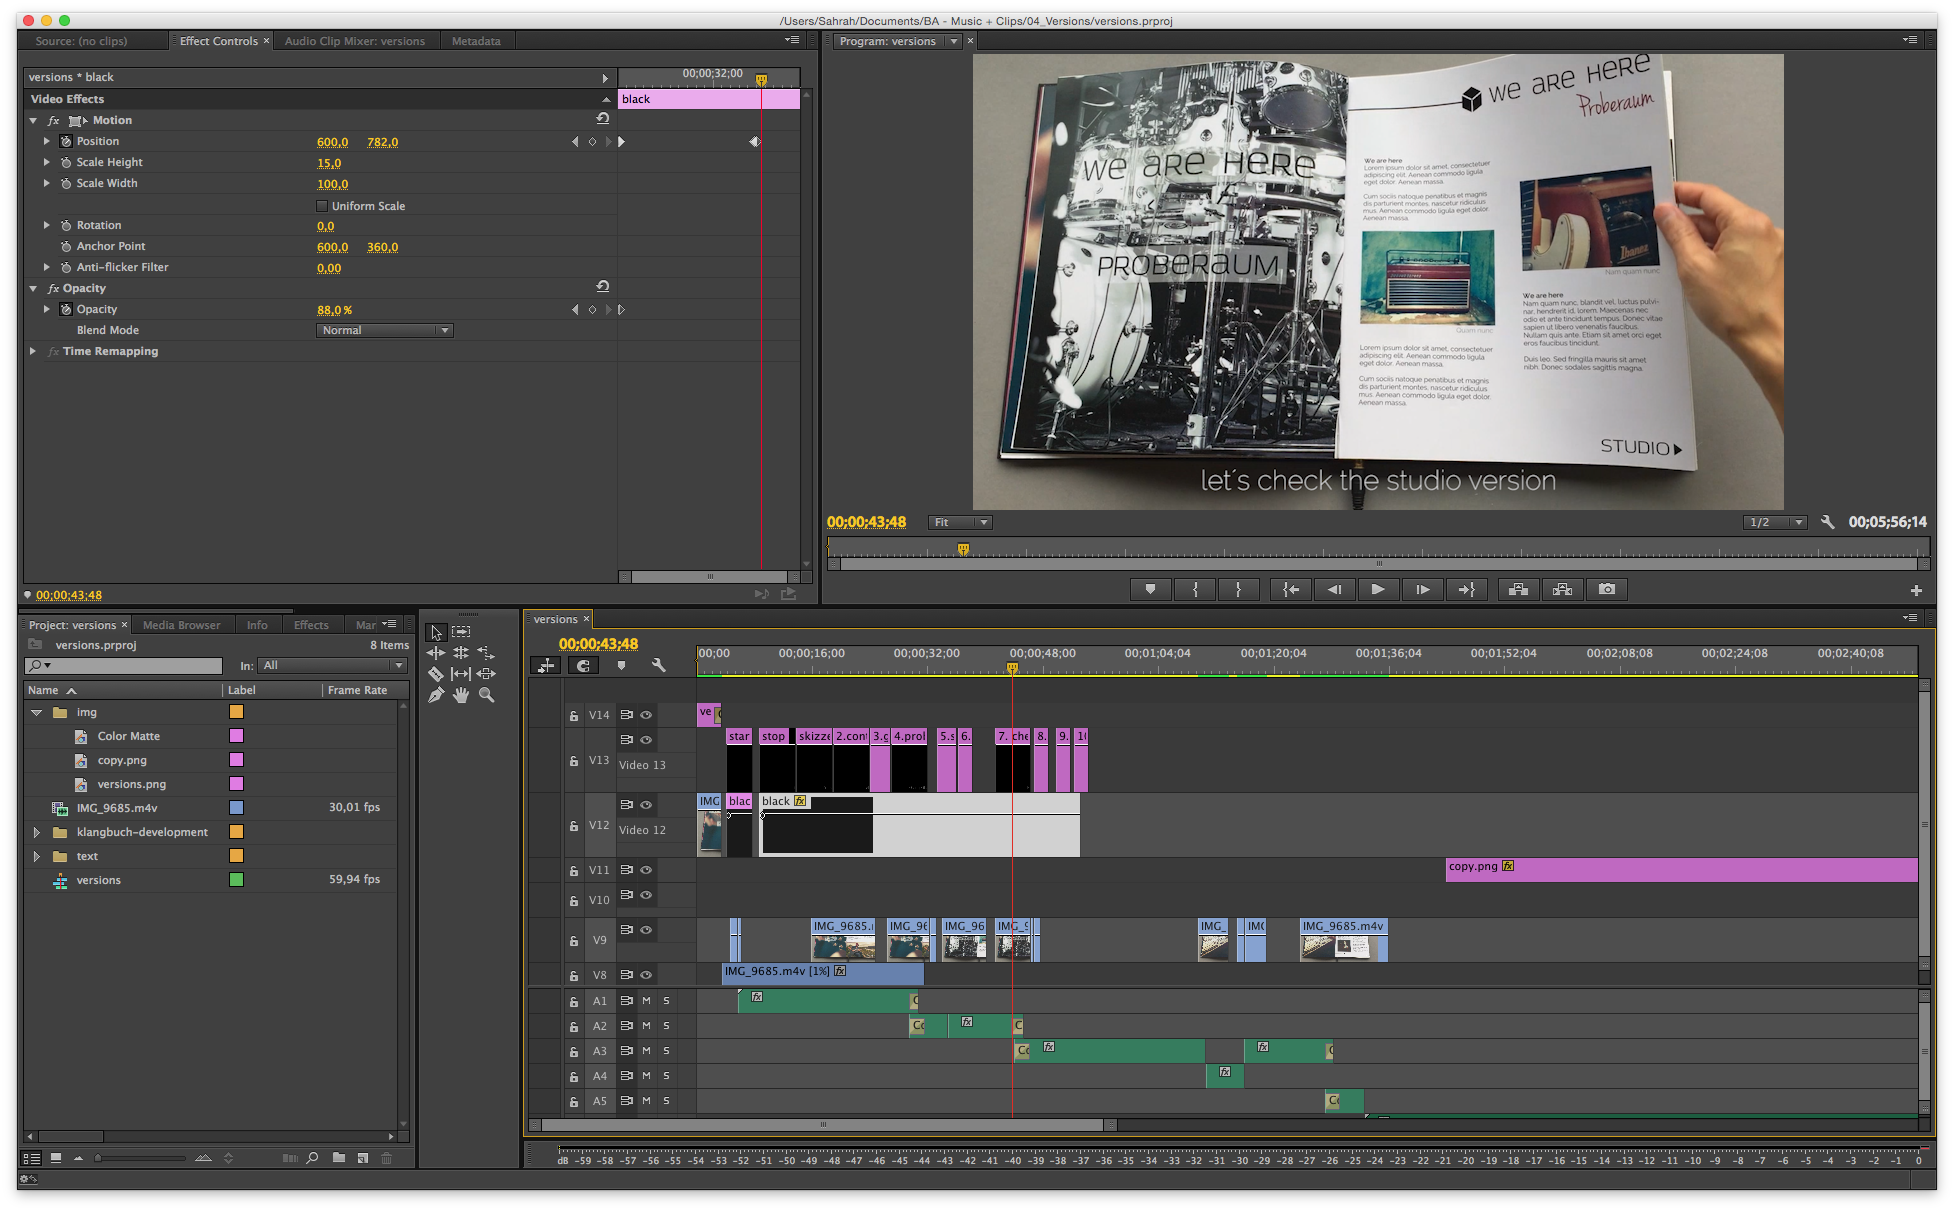
\includegraphics[width=0.8\textwidth]{grafiken/montagefilm.png}
\caption{Montage des \gls{clip}s "Versions"}
\end{figure}


\section{Video-Einbindung}
Die Videos sollten in der Website so eingebunden werden, dass sie von möglichst vielen Browsern auf möglichst vielen Endgeräten abgespielt werden können. Um dieses Ziel zu erreichen, bietet es sich an die Videos über ein Videoportal bereit zu stellen. Videoportale konvertieren die Videos beim Hochladen automatisch in ein browserübergreifendes, webtaugliches Format und betten diese in einen Videoplayer ein. Die Videos sind dann nahezu auf jedem Endgerät abspielbar. Über ein iFrame können die Videos dann in die Website eingebunden werden.\\

\subsection{Auswahl Video-Portal}
Der Video-Kanal muss für die Bachelorarbeit folgende Kriterien erfüllen:

\begin{itemize}
\item Anbieten aller benötigten Funktionen zu einem möglichst geringen Preis
\item Hochladen von mind. vier Videos
\item Möglichkeit zur Einbindung der Videos in eine Website
\item Möglichkeit die Videos nicht zu listen\footnote{Videos nicht listen: Das Hochladen von Videos in Videoportalen bedeutet, dass sie für jeden Internetnutzer sichtbar sind. Durch das Nichtlisten sind die hochgeladenen Videos nicht frei zugänglich, sondern können nur über eine bestimmte URL erreicht werden. Da das Gesamtprojekt "Digitale Klangbuch" noch in der Entwicklung ist, sollten die Videos zum aktuellen Zeitpunkt nicht für jeden frei zugänglich sein.}
\end{itemize}


Das bekannteste Videoportal ist YouTube\footnote{YouTube: \url{http://www.youtube.com}}\cite{statYT}. YouTube erfüllt alle genannten Kriterien und bietet diese Funktionen zudem kostenlos an.\\
Eine Alternative ist das Videoportal Vimeo\footnote{Vimeo: \url{http://www.vimeo.com}}. Anders als bei YouTube ist das Hochladen von Videos bei Vimeo nur gestattet, wenn diese selbst produziert sind und alle erforderlichen Rechte bei einem liegen. Damit richtet sich Vimeo eher an Künstler und Filmproduzenten, während YouTube keine spezielle Zielgruppe hat.\cite{chip} Das Nichtlisten von Videos ist bei Vimeo nur mit einer Pro-Mitgliedschaft für 159 \euro /Jahr möglich, weshalb Vimeo nicht alle Kriterien erfüllt. Da das digitale Klangbuch noch in der Entwicklung ist, sollten die Videos zum aktuellen Zeitpunkt nicht für jeden frei zugänglich sein. Der Videokanal wird auf YouTube erstellt. Für die Zukunft sollte jedoch auch ein Videokanal bei Vimeo eingerichtet werden.\\

Der Video-Kanal ist unter folgendem Link erreichbar:\\\url{https://www.youtube.com/channel/UCJ_SsBh-EhDPPo9xxOF2MVQ}\\
Die Videoclips können ebenfalls von der CD, die der gebundenen Ausgabe der Bachelorarbeit beiliegt, abgespielt werden.


\begin{figure}[H]
\centering

\includegraphics[width=0.8\textwidth]{grafiken/youtubekanal.png}
\caption{YouTube Kanal "Digitales Klangbuch"}
\end{figure}

%%%%%%%%%%%%%%%%%%%%%%%%%%%%%%%%%%%%
%%%%%%%%%%%%%%%%%%%%%%%%%%%%%%%%%%%%

\section{Website}

Für die Entwicklung der Website wurden fertige Template-Sets recherchiert. Das Template-Set soll folgenden Anforderungen entsprechen:\\

\textbf{Inhalte einbinden}\\
Das Einbinden von Texten, Grafiken und Videos soll möglich sein.\\

\textbf{Leicht verständlich \& schlicht}\\
Das Template-Set soll den Aufwand der Entwicklung und des Testings der Website möglichst gering halten. Daher soll es vom Aufbau und Einstieg in die Entwicklung leicht verständlich und schlicht sein.\\

\textbf{\gls{responsive}}\\
Das Template-Set soll responsive aufgebaut sein. Neu hinzugefügte Elemente sollen ebenfalls problemlos responsive eingebunden werden können.\\

\textbf{Editierbar- \& Erweiterbarkeit}\\
Das Template-Set soll einfach editierbar und erweiterbar sein. HTML-, PHP-, Javascript- und \Gls{stylesheet}-Dateien sollen verändert werden können. Das erstellte Design mit Farben, Schriften, Logos soll in das Template-Set integriert werden können.\\

\textbf{Lizenzfrei}\\
Um Kosten zu vermeiden, soll das Template-Set möglichst lizenzfrei sein.\\


Die Wahl fiel auf ein \gls{onepager} Template-Set von "HTML5 UP"\footnote{HTML5 UP: \url{http://www.html5p.net}}. Der Vorteil an einem \gls{onepager}  liegt darin, dass alle Informationen, Funktionen und Videos auf einer Seite ohne Navigation zu finden sind. Durch Scrolling der Seite wird der Nutzer in eine bewusst gesteuerte Reihenfolge durch die Inhalte der Seite geführt.


\subsection{Anpassung Website}
Das \Gls{stylesheet} der Webseite wurde an die Farben und Schriften des entwickelten Designs angepasst. Das Einbinden der Schrift Oxygen konnte über die Api von Google-Font erfolgen.

\begin{lstlisting}
<link href='https://fonts.googleapis.com/css?family=Oxygen:400,300,700'
rel='stylesheet' type='text/css'>
\end{lstlisting}

\vspace{0.5cm}

Die Schrift Azoft musste separat hochgeladen und über das \Gls{stylesheet} eingebunden werden.

\begin{lstlisting}
@font-face{
	font-family: 'azoft';
	src: url("../fonts/azoft-sans.ttf");
}

@font-face{
	font-family: 'azoft';
	src: url("../fonts/azoft-sans-bold.ttf");
	font-weight: bold;
}
\end{lstlisting}


Das Template-Set berücksichtigt nicht das responsive Einbinden von Videos. Dies ließ sich jedoch über einen Open-Source \Gls{stylesheet} Code realisieren:

\begin{lstlisting}
// Embeds responsive
// Credit: Nicolas Gallagher and SUIT CSS.

.embed-responsive {
  position: relative;
  display: block;
  height: 0;
  padding: 0;
  overflow: hidden;

  .embed-responsive-item,
  iframe,
  embed,
  object,
  video {
    position: absolute;
    top: 0;
    left: 0;
    bottom: 0;
    height: 100%;
    width: 100%;
    border: 0;
  }
}

// Modifier class for 16:9 aspect ratio
.embed-responsive-16by9 {
  padding-bottom: 56.25%;
}
\end{lstlisting}


\subsection{Testen der Website}
Die Website wurde auf verschiedene Browser und Endgeräte getestet und angepasst.\\
\textbf{Getestete Browser}: Google Chrome, Safari, Firefox.\\
\textbf{Getestete Endgeräte}: Apple iPad, Apple iPhone 6, Google Nexus\\


Screenshots zur Webseite können im Anhang eingesehen werden.
Die Website ist unter folgender URL zu erreichen: \url{http://www.klangbuch.net}


%TODOs:\\
%\begin{itemize}

%\item Glossar vervollständigen
%\item Was ist eigentlich ein Erlebnis?
%\item Beispiele für Gesamtkunstwerk\\Pink Floyd - Pulse 2 Album ?\\Mogwai - Rave Tapes?
%\item Überall Klangbuch Schreibweise checken
%\item Ganz am Ende die Bib + Glossar neu erstellen + alle Begriffe im Dok hinzufügen

%\end{itemize}












%%!TEX root = ../PP.tex

\newcommand{\fFunktionen}{040_funktionen}

\part{Der Leitfaden}

\textbf{Der Leitfaden - Beschreibung}\\
Dieser Teil erläutert die Möglichkeiten und Grenzen des digitalen Klangbuchs. Es werden Darstellungsmöglichkeiten und Funktionen erarbeitet. Arten von Leitfäden werden diskutiert und ein Leitfaden konzipiert und umgesetzt.

%!TEX root = ../PP.tex

%TODO: 

\chapter{Möglichkeiten und Grenzen des digitalen Klangbuchs}\label{moeglichkeiten}

Bevor ein Leitfaden und Funktionen für das digitale Klangbuch entwickelt werden können, müssen zuvor die Möglichkeiten und Grenzen des digitalen Klangbuchs erläutert werden. Im Folgenden wird das digitale Klangbuch mit seinen technischen Möglichkeiten und Grenzen kurz skizziert.


%%%%%%%%%%%%
%%%%%%%%%%%%

\section{Technik im digitalen Klangbuch}

Im Praxisprojekt wurden unterschiedliche Realisierungsansätze vorgestellt. Die Ansätze präsentierten dabei verschiedene Technologien und Möglichkeiten zum Aufbau des Buches. Um den Rahmen der Bachelorarbeit nicht zu sprengen, beschränkt sie sich auf folgende Technologien und Hilfsmittel, die bei der Funktionsentwicklung und der Entwicklung des Leitfadens im digitalen Klangbuch eingesetzt werden:


\begin{itemize}
\item{Leitende Tinte}
\item{Leitender Kleber}
\item{Gedruckte Elektronik}
\item{SMD-LEDs}
\end{itemize}

\textbf{Leitende Tinte} ist eine Flüssigkeit, mit der sich funktionierende Stromkreise auf Papier zeichnen und drucken lassen. Aufgrund des körpereigenen Widerstands ist die Tinte berührungsempfindlich. Dadurch lassen sich Bedienelemente direkt auf das Papier drucken.\\

Unter \textbf{gedruckte Elektronik} versteht man elektronische Bauteile, die über ein spezielles Verfahren auf ein Trägermaterial aufgedruckt werden können. Ein zentraler Ansatz im digitalen Klangbuch ist die Erkennung der Seite, auf der sich der Hörer gerade befindet. Dadurch lassen sich Funktionen, die nur auf einer bestimmten Seite möglich sind, steuern. Z. B. das automatische Starten eines Songs, sobald eine spezielle Seite umgeblättert wird. Ein gedruckter Sensor ist für die Seitenerkennung notwendig. Der Sensor ist nicht sichtbar zwischen zwei Seiten eingebettet und taucht deshalb nicht in den Skizzen der Funktionsbeschreibungen auf.\\


\textbf{Leitender Kleber} ist ein Klebstoff, der Strom leitet. Damit lassen sich Elemente, die an einen Stromkreis angeschlossen werden müssen, über den Klebstoff integrieren, z. B. SMD-LEDs. Der Kleber wiederum wird mit leitender Tinte verbunden.\\


\textbf{SMD-LEDs} sind winzig kleine LEDs, die ohne Drähte auskommen. Sie können mit dem leitenden Kleber direkt auf das Papier des Klangbuchs aufgeklebt werden. Die kleinste Bauform misst eine Größe von 1,0 x 0,5 x 0,45 mm.\\


%%%%%%%%%%%%


\section{Aufbau Digitales Klangbuch}
In Abbildung \ref{fig:aufbauBuch} ist der Aufbau des digitalen Klangbuchs skizziert: Im hinteren Buchdeckel ist die Technik zur Steuerung eingebettet (1). Der Buchrücken (3) ist mit den Komponenten im Buchdeckel verbunden. Auf den einzelnen Seiten des Buches können mit leitender Tinte berührungsempfindliche Elemente (2.1) gedruckt und mit leitendem Kleber SMD-LEDs (2.2) integriert werden. Jede SMD-LED und jedes berührungsempfindliche Element muss mit leitender Tinte mit dem Buchrücken verbunden werden.


\begin{figure}[H]
\centering
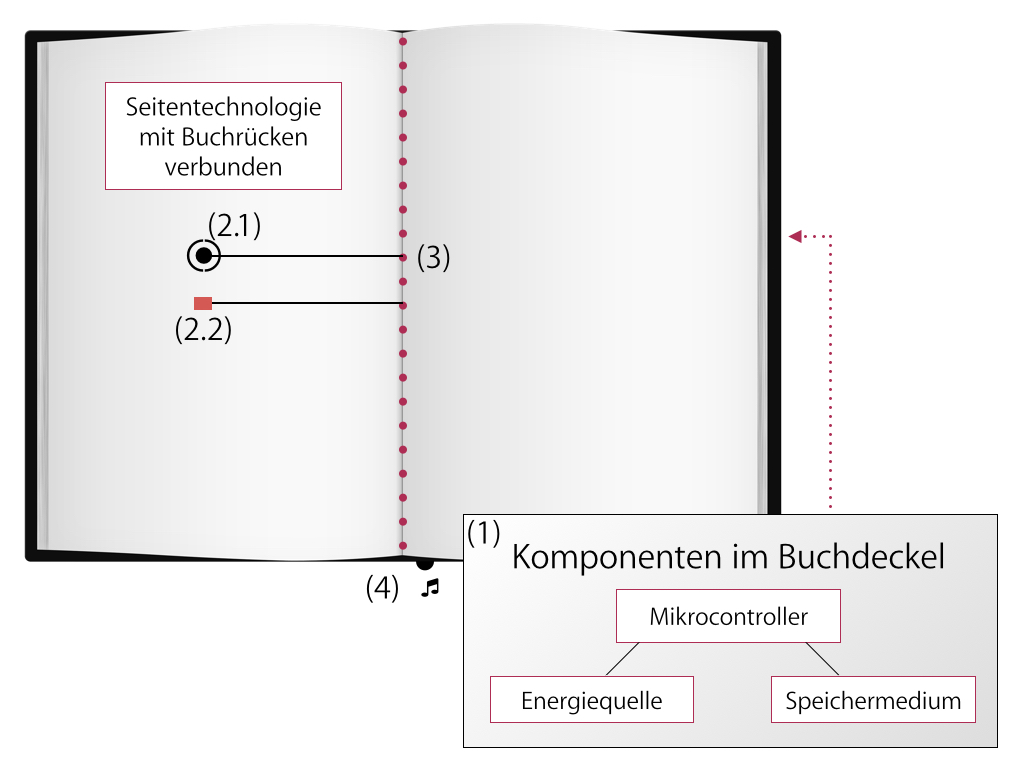
\includegraphics[width=1.0\textwidth]{grafiken/aufbau-klangbuch.jpg}
\caption{Aufbau des digitalen Klangbuchs: (1) Technik im Buchdeckel, (2.1) berührungsempfindliches Element, (2.2) SMD-LED, (3) Buchrücken, (4) Audioausgang }
\label{fig:aufbauBuch}
\end{figure}


\section{Möglichkeiten \& Grenzen}

\subsection{Möglichkeiten}
Durch den Einsatz der zuvor beschriebenen Technik, ist es möglich Audiodaten abzuspielen, SMD-LEDs anzusteuern und Interaktionen auszuwerten (Berührung eines berührungsempfindlichen Elements). Die Auswertung der Interaktion kann für den Hörer in zwei Formen sichtbar gemacht werden:\\
1. Eine Interaktion bewirkt eine eine akustische Veränderung: ein Klang ertönt oder verstummt (z. B. wird ein Song beim Berühren eines bestimmten Elements gestartet).\\
2. Eine Interaktion bewirkt eine visuelle Veränderung: eine oder mehrere SMD-LEDs beginnen zu leuchten, verdunkeln, blinken oder ändern ihren Farbwert.

\subsection{Grenzen}
Berührungsempfindliche Elemente werden mit spezielle, leitende Tinte auf die Seiten des Buches gedruckt. Diese Elemente und jede integrierte SMD-LED werden durch Linien aus gedruckter leitender Tinte mit dem Buchrücken verbunden. Bei der Erstellung der Layouts müssen diese Elemente und Linien berücksichtigt werden. Dabei ist auch zu beachten, dass die Linien ebenfalls auf Berührung reagieren und sie sich auch gegenseitig nicht berühren dürfen.



%%%%%%%%%%%%%%%%%%%%%%%%%%%%%%%%%%%%%%%%%%%%%%%%%%%%%%%%%%%%%%%%%%%%%%%%%%%%%%%%%%%%%%%%%%%%%%%%
%%%%%%%%%%%%%%%%%%%%%%%%%%%%%%%%%%%%%%%%%%%%%%%%%%%%%%%%%%%%%%%%%%%%%%%%%%%%%%%%%%%%%%%%%%%%%%%%
%%%%%%%%%%%%%%%%%%%%%%%%%%%%%%%%%%%%%%%%%%%%%%%%%%%%%%%%%%%%%%%%%%%%%%%%%%%%%%%%%%%%%%%%%%%%%%%%
%%%%%%%%%%%%%%%%%%%%%%%%%%%%%%%%%%%%%%%%%%%%%%%%%%%%%%%%%%%%%%%%%%%%%%%%%%%%%%%%%%%%%%%%%%%%%%%%
%%%%%%%%%%%%%%%%%%%%%%%%%%%%%%%%%%%%%%%%%%%%%%%%%%%%%%%%%%%%%%%%%%%%%%%%%%%%%%%%%%%%%%%%%%%%%%%%


\chapter{Darstellungs- und Funktionsmöglichkeiten}\label{funktionen}

Das digitale Klangbuch spricht den haptischen, visuellen und akustischen Sinn an. Im Folgenden werden Ideen und Funktionen entwickelt. Diese werden in folgende Bereiche unterteilt: Interaktion (haptische Wahrnehmung), Darstellungsmöglichkeiten (visuelle Wahrnehmung) und Akustik (auditive Wahrnehmung).

%%%%%%%%%%%%
%%%%%%%%%%%%
%%%%%%%%%%%%

\section{Interaktion}
Das digitale Klangbuch ermöglicht es dem Hörer interaktiv mit dem Buch und dessen Inhalte zu agieren.

\subsection{Berührungsempfindliche Elemente}
Elemente, die mit leitender Tinte gedruckt und mit dem Buchrücken verbunden wurden, sind berührungsempfindlich. Bei Berührung können sie eine Funktion auslösen, z. B. das Starten eines Songs. Durch logische Verknüpfungen ist es auch möglich berührungsempfindliche Elemente miteinander zu verketten. Ein Beispiel: Berührung von Element A löst Funktion a aus. Berührung Element B, löst Funktion b aus. Berührung von Element A und B zu gleicher Zeit, löst Funktion c aus.

\subsection{Umblättern einer Seite}
Die Seiten des digitalen Klangbuchs sind mit Sensoren ausgestattet. Wird eine Seite umgeblättert, registriert der Sensor auf welcher Seite sich der Hörer befindet. Es kann dann eine Funktion ausgelöst werden, z. B. das Starten eines Songs.


%%%%%%%%%%%%
%%%%%%%%%%%%
%%%%%%%%%%%%

\section{Darstellungsmöglichkeiten}

Im digitalen Klangbuch ist an Inhalten alles möglich, was ein herkömmliches Buch bietet: Raum für Geschichten, Bilder, Illustrationen, Texte, etc. Kombiniert mit der Technik, den Interaktionsmöglichkeiten und der Musik bzw. Audioinhalten, lassen sich unzählige, neuartige Inhalte generieren. Denkbar wären z. B.:

\begin{itemize}
\item Entstehungsgeschichte des Musikers / der Band, begleitet von Musik, Audiokommentaren, etc.
\item Informationen und Geschichten über den Musiker / der Band
\item Bedeutung, die hinter einem ausgewählten Songs steht
\item Entstehungsprozess eines ausgewählten Songs
\item bisherige Veröffentlichungen, \gls{remix}e, etc.
\item Lyriktexte der Songs
\item Fotos des Musikers / der Band
\item Zeichnungen, Bilder, Illustrationen
\end{itemize}

Die Seiten des digitalen Klangbuchs bestehen aus gängigem Fotopapier. Sie können nach Wünschen des Künstlers farbig bedruckt werden. So können Fotos, Grafiken, künstlerische Werke, Texte, etc. auf die Seiten gedruckt werden. Es ist ebenfalls möglich spezielle Techniken aus der Buchkunst zu integrieren, z. B. Pop Up´s\footnote{Pop Up Kunst bezeichnet Elemente, die durch eine besondere Falttechnik räumlich herausspringen (pop up).} (s. Abbildung \ref{fig:Popup}) und diese ebenfalls mit leitender Tinte und SMD-LEDs zu kombinieren (s. Abbildung \ref{fig:PopupLED}.\\


\begin{figure}[H]
\centering
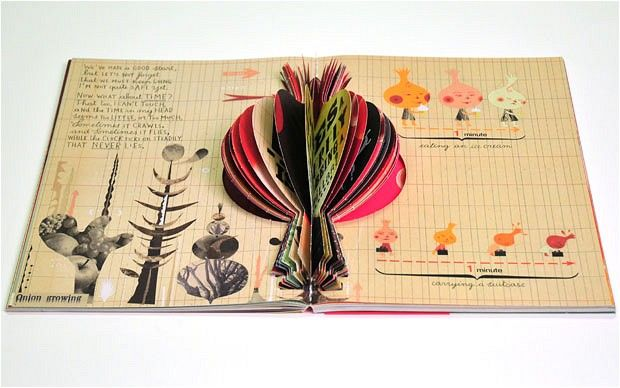
\includegraphics[width=0.8\textwidth]{grafiken/popup.jpg}
\caption{Pop Up Kunst in einem Buch.\\Foto: The Onion’s Great Escape by Sara Fanelli, Portia Webb, \url{http://www.telegraph.co.uk/culture/books/children_sbookreviews/9682987/Books-for-Christmas-childrens-books.html} }
\label{fig:Popup}
\end{figure}


\subsection{Leuchtende Elemente}
Durch eingesetzte SMD-LEDs ist es möglich Veränderungen visuell anzuzeigen und so Informationen zu transportieren. Eine SMD-LED kann blinken, leuchten und die Farbe wechseln. So können z. B. SMD-LEDs auf einer Zeitleiste angeordnet werden, welche dem Hörer durch Blinken anzeigt, an welcher Stelle sich der Song gerade befindet.


\begin{figure}[H]
\centering
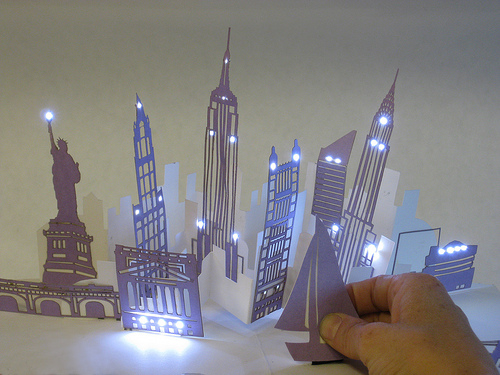
\includegraphics[width=0.5\textwidth]{grafiken/popupled.jpg}
\caption{Pop Up Kunst mit LEDs.\\Foto: Electronic Popables, high-low tech, \url{http://highlowtech.org/?p=5} }
\label{fig:PopupLED}
\end{figure}


\subsection{Grenzen im Layout}
Berührungsempfindliche Elemente werden mit spezieller, leitender, schwarzer Tinte auf die Seiten des Buches gedruckt. Diese Elemente und jede integrierte SMD-LED werden durch Linien aus gedruckter leitender Tinte mit dem Buchrücken verbunden. Bei der Erstellung der Layouts müssen diese Elemente und Linien berücksichtigt werden. Dabei ist auch zu beachten, dass die Linien ebenfalls auf Berührung reagieren und sie sich auch gegenseitig nicht berühren dürfen.

\begin{figure}[H]
\centering
\includegraphics[width=0.8\textwidth]{grafiken/bspklangbuch.png}
\caption{Beispiel Layout eines digitalen Klangbuchs: Berührungsempfindliche Elemente werden mit Linien aus leitender Tinte mit dem Buchrücken verbunden. Die Linien dürfen sich nicht kreuzen.}
\end{figure}




%%%%%%%%%%%%
%%%%%%%%%%%%
%%%%%%%%%%%%

\section{Akustik}
Ein herkömmliches CD-/DVD-/Blueray-Album bietet dem Fan in manchen Fällen auch Bonusmaterial. Das Bonusmaterial ist vor allem auf der CD begrenzt und besteht oft nur aus einem zusätzlichen Song, z. B. ein \gls{remix}. Mit dem digitalen Klangbuch soll das herkömmliches Album um Funktionen und Inhalte erweitert werden. In diesem Kapitel werden Funktionen und Ideen vorgestellt, die vor allem den akustischen Sinn des Fans ansprechen sollen. 


\subsection{Audio abspielen}
Die grundlegendste Funktion ist die Möglichkeit ein Audiostück zu starten, zu stoppen, zu pausieren und die Lautstärke zu regeln.\\


\textbf{Unterschied zum herkömmlichen Album}\\
Der Hörer berührt im digitalen Klangbuch Elemente, die auf eine Papierseite aufgedruckt sind. Dadurch wird der haptische und der auditive Sinn angesprochen.\\

\textbf{Erweiterte Funktionsmöglichkeit}\\
Die Veränderungen können durch SMD-LEDs angezeigt werden, wodurch auch eine visuelle Änderung wahrgenommen werden kann.


%%%%%%%%%%%%


\subsection{Sprachwahl}
Die Gesangsspur eines Songs kann über eine Auswahl in einer anderen Sprache abgespielt werden.\\


\textbf{Unterschied zum herkömmlichen Album}\\
Ein Song, der Gesang oder Sprache enthält, wird für gewöhnlich in einer ausgewählten Sprache gesungen / gesprochen. Selten hat der Hörer die Möglichkeit den Song auch in einer anderen Sprache zu hören. Der KlangKünstler kann dem Hörer eine Auswahl an Spuren in unterschiedlicher Sprache anbieten.\\


\textbf{Weiteres Nutzungsszenario}\\
Dem Hörer kann es möglich sein die Gesangsspur durch eine eigene zu ersetzen.



%%%%%%%%%%%%


\subsection{Interview}
Statt eines Songs, können auch Interviews des KlangKünstler hinterlegt werden.\\


\textbf{Unterschied zum herkömmlichen Album}\\
Im Gegensatz zu einem kleinformatigem \gls{booklet}, können die Interviews im großformatigen digitalen Klangbuch ausführlich grafisch begleitet werden. So kann der Fan zu vielen Details im Interview visuell bedient werden.\\


\textbf{Weiteres Nutzungsszenario}\\
Anhand von SMD-LEDs können visuelle Inhalte des Buches (Bilder, Texte, etc.) passend zu den Stellen des Interviews deutlich gemacht werden.



%%%%%%%%%%%%


\subsection{Equalizer - Presets}
Eine weitere Grundfunktion, die in gängigen Geräten zum Abspielen von Audio enthalten ist, ist ein Equalizer. Er dient dazu um den Klang an die eigenen Wünsche anzupassen: Höhen, Tiefen, etc. Das digitale Klangbuch kann hierzu sogenannte Presets, parametrische Voreinstellungen des Equalizers, anbieten.\\

\textbf{Unterschied zum herkömmlichen Album}\\
Der Hörer berührt im digitalen Klangbuch Elemente, die auf einer Papierseite aufgedruckt sind. Dadurch wird der haptische und der auditive Sinn angesprochen.\\

\textbf{Erweiterte Funktionsmöglichkeit}\\
Die Veränderungen können durch SMD-LEDs angezeigt werden, wodurch auch eine visuelle Änderung wahrgenommen werden kann.


%%%%%%%%%%%%

\subsection{\gls{remix}e}
Der Hörer kann sich zu einem Song verschiedene \gls{remix}e anhören.\\

\textbf{Unterschied zum herkömmlichen Album}\\
Im Gegensatz zu einem kleinformatigem \gls{booklet}, können die \gls{remix}e im großformatigen digitalen Klangbuch ausführlich grafisch begleitet werden.


%%%%%%%%%%%%
%%%%%%%%%%%%
%%%%%%%%%%%%


\subsection{Multitrack}
Multitrack bedeutet zu deutsch "Mehrspur". Es bietet die Möglichkeit einen Song in mehreren, separaten Spuren abzuspielen und diese bei Bedarf einzeln stummzuschalten, auszutauschen oder zu bearbeiten.\\

\textbf{Unterschied zum herkömmlichen Album}\\
Der Hörer hat hier die Möglichkeit einzelne Spuren stumm zu schalten und die Lautstärke der Spuren einzeln zu verändern.\\

\textbf{Erweiterte Funktionsmöglichkeit}\\
Dem Hörer kann es möglich sein eine der Spuren, z. B. die Gesangsspur, durch eine eigene zu ersetzen.


%%%%%%%%%%%%


\subsection{SongKit}
Als SongKit ist in diesem Kontext ein Bausatz zu verstehen, der verschiedene \gls{loop}s einer Klangspur zur Verfügung stellt. Die Idee dahinter ist, ein Musikstück des Albums in seine Spuren zu teilen - beispielsweise in Bass, Drums, Melodie, Gesang - und diese in einer Dauerschleife abspielen zu lassen. Zu jeder Spur gibt es Alternativen, die ausgewählt werden können. So kann der ursprüngliche Song verändert werden.\\


\textbf{Unterschied zum herkömmlichen Album}\\
In der Produktionsphase eines Songs verändert sich der Song von der Idee bis zum fertigen Song. Andere Versionen des Songs, z. B. mit einer anderen Basspur, bekommt der Musikfan nahezu nie zu hören. Durch das SongKit im Klangbuch können diese Versionen integriert werden. Dabei kann der Hörer selbst bestimmen, welche Spuren er zusammen mischt.\\


\textbf{Weiteres Nutzungsszenario}\\
Das SongKit kann unabhängig vom Album eine Auswahl an \gls{loop}s bereit stellen. Das heißt, die \gls{loop}s müssen nicht zwingend einen Bezug zu dem Album oder einem Song haben. Die KlangKünstler können einen Baukasten mit passenden \gls{loop}s zusammen stellen, die der Hörer dann nach seinen Wünschen zu einem Song-\gls{loop} zusammen stellt.



%%%%%%%%%%%%


\subsection{Audiokommentare}
Zu einem Song können Audiokommentare hinterlegt werden, die sich der Hörer bei Bedarf anhören kann. Die Audiokommentare können in einer Timeline, passend zum Song, hinterlegt werden. Aktiviert der Hörer die Audiokommentare, reduziert sich die Lautstärke des bereits laufenden Songs, sodass die entsprechenden Audiokommentare an den passenden Stellen erklingen können. \\


\textbf{Unterschied zum herkömmlichen Album}\\
Audiokommentare sind selten in einem gewöhnlichen Musikalbum zu finden.\\


\textbf{Weiteres Nutzungsszenario}
\begin{itemize}
\item Variation 1: Audiokommentare können über einzelne \gls{button}s individuell gestartet werden.
\item Variation 2: Die Kommentare können als Texte im Buch hinterlegt werden. Erreicht der laufende Song einen Audiokommentar, leuchtet eine dazu platzierte SMD-LED auf. Ein ähnliches Konzept findet sich auf Soundcloud\footnote{Soundcloud ist ein Online-Musikdienst für Musiker zum Anbieten von Audiodateien. Fans können auf der Zeitleiste eines Songs zu jeder Sekunde einen Kommentar hinterlassen.}.
\end{itemize}


%%%%%%%%%%%%


\subsection{Interaktiver Song}
In interaktiven Videos\footnote{Interaktives Videobeispiel: Ink von Colplay\cite{CO}} ist es möglich den Handlungsstrang zu beeinflussen. Der Verlauf eines Songs kann über das digitale Klangbuch ebenfalls durch den Hörer bestimmt werden. Ein Beispiel dazu wird in der Skizze - Abbildung \ref{fig:abb1} veranschaulicht.\\
Beim Öffnen der Seite wird der Song automatisch gestartet. Die Zeitleiste (a) symbolisiert die Länge des Songs. Der Hörer hat nun die Möglichkeit den Verlauf des Songs, während dieser bereits spielt, zu ändern. Dazu wurde der Song in drei Bereiche geteilt (Minute 0:30, 1:30 und 2:30). Diese Bereiche werden im Folgenden "Kapitel" genannt.\\ 

Der Hörer hat die Möglichkeit in jedem Kapitel den Verlauf des Songs zu verändern:
\begin{itemize}
\item Kapitel 1: Der Song kann eine dramatische, eine ruhige oder eine rätselhafte Richtung einschlagen.
\item Kapitel 2: Die Gesangsstimme kann männlich, weiblich oder die eines Kindes sein.
\item Kapitel 3: Das Ende des Songs kann mitbestimmt werden - ein fröhliches, ein zerstörtes oder überhaupt kein Ende, sodass der Song von neuem beginnt.
\end{itemize} 

SMD-LEDs (b) zeigen dem Hörer an, wie lang es ihm möglich ist den Verlauf für dieses Kapitel zu ändern. Solange die SMD-LED in einem der Kapitel leuchtet, kann der Hörer den Verlauf bestimmen.


\begin{figure}[H]
\centering
\includegraphics[width=1.0\textwidth]{grafiken/function_interactivesong.png}
\caption{Beispiel-Skizze Interaktiver Song im digitalen Klangbuch}
\label{fig:abb1}
\end{figure}


\textbf{Unterschied zum herkömmlichen Album}\\
Interaktive Songs sind nicht neu. Auf einem Album kann diese Idee jedoch nicht verwirklicht werden. Im Internet gibt es Beispiele zu interaktiven Songs z. B. auf dem Videoportal YouTube\footnote{Interaktiver Song auf YouTube: \url{https://www.youtube.com/watch?v=OtcpO4vipNU}} und dem Storytelling Tool interlude\footnote{interlude:\url{http://blog.interlude.fm/}}.\\


\textbf{Weiteres Nutzungsszenario}
\begin{itemize}
\item Ideenbeispiel 1: Der Interaktive Song kann auf mehrere Seiten im Buch ausgeweitet werden. So kann der Inhalt der Seiten auf jeden "Handlungsstrang" angepasst werden.
\item Ideenbeispiel 2: Der Song kann eine Geschichte erzählen, sowohl grafisch, als auch über den Songtext. Je nach gewählten Handlungsstrang, kann die Geschichte eine andere Wendung nehmen, der Songtext ändert sich. Die verschiedenen Songtexte können im Klangbuch abgebildet und vom Hörer mitgelesen werden.
\end{itemize}



%%%%%%%%%%%%


\subsection{Entstehungsgeschichte Song - "Versions"}
Die Entstehungsgeschichte eines Songs, im Folgenden auch "Versions" genannt, kann im digitalen Klangbuch nicht nur durch Texte und passende Bilder erzählt werden. Der Hörer kann auch in die verschiedenen Versionen, die ein Song von der Idee hin zu einer Live-Version durchläuft, hinein hören. Beispielstationen bei der Entwicklung eines Songs sind folgende:

\begin{itemize}
\item Skizze: Die erste Idee, die auf einem Klavier oder einer Gitarre entsteht
\item Proberaumversion: Die weiter verarbeitete Idee, die mit der Band im Proberaum verfeinert wird
\item Studioversion: Der Song wird professionell in einem Studio aufgenommen
\item Live-Version: Eine Aufnahme, die auf einem Live-Konzert mitgeschnitten wurde
\end{itemize}  


\textbf{Unterschied zum herkömmlichen Album}\\
Der Hörer kennt oftmals nur die Studio- oder Live-Version eines Songs. Der Entstehungsprozess bleibt dabei meist außen vor.\\


%%%%%%%%%%%%%%%%%%%%%%%%%%%%%%%%%%%%%%%%%%%%%%%%%%%%%%%%%%%%%%%%%%%%%%%%%%%%%%%%%%%%%%%%%%%%%%%%
%%%%%%%%%%%%%%%%%%%%%%%%%%%%%%%%%%%%%%%%%%%%%%%%%%%%%%%%%%%%%%%%%%%%%%%%%%%%%%%%%%%%%%%%%%%%%%%%
%%%%%%%%%%%%%%%%%%%%%%%%%%%%%%%%%%%%%%%%%%%%%%%%%%%%%%%%%%%%%%%%%%%%%%%%%%%%%%%%%%%%%%%%%%%%%%%%
%%%%%%%%%%%%%%%%%%%%%%%%%%%%%%%%%%%%%%%%%%%%%%%%%%%%%%%%%%%%%%%%%%%%%%%%%%%%%%%%%%%%%%%%%%%%%%%%
%%%%%%%%%%%%%%%%%%%%%%%%%%%%%%%%%%%%%%%%%%%%%%%%%%%%%%%%%%%%%%%%%%%%%%%%%%%%%%%%%%%%%%%%%%%%%%%%


\chapter{Leitfäden: Arten und Auswahl eines Leitfadens}

Ziel ist es einen Leitfaden zu entwickeln, der die Funktionen und Möglichkeiten des digitalen Klangbuchs erläutert und veranschaulicht. Dem KlangKünstler sollen die Möglichkeiten und der multisensuale Charakter des digitalen Klangbuchs verdeutlicht und Nahe gebracht werden.\\

Im Folgenden werden mögliche Arten von Leitfäden vorgestellt. In einer Bewertungstabelle werden diese anhand von Kriterien gegenüber gestellt und ausgewertet. Anschließend wird ein Leitfaden erstellt.

%%%%%%%%%%%%
%%%%%%%%%%%%
\section{Arten von Leitfäden}



%%%%%%%%%%%%

\subsection{Leitfaden als gedrucktes Handbuch}
Ein gedrucktes Handbuch enthält die Funktionen eines Produkts und beschreibt diese ausführlich. Es dient als Dokumentation, Nachschlagewerk und Anleitung, in dem Bilder und Texte platziert werden können.\\

\textbf{Vorteile}\\
Das Handbuch ist ein gängiges Format zur detaillierten Beschreibung von Funktionen. Der Leitfaden in Form eines gedruckten Handbuchs ließe sich in der Bachelorarbeit realisieren.\\

\textbf{Nachteile}\\
Der Nachteil eines Handbuches ist, dass der KlangKünstler die Funktionsmöglichkeiten nicht aktiv erleben kann: es fehlen Klangbeispiele und Interaktionen, die das Klangbuch ausmachen. Ein gedrucktes Handbuch bietet keine interaktive Suche an. Es ermöglicht nur eine eine Suche über einen abgedruckten Wortindex. Ein gedrucktes Handbuch verliert sehr schnell an seiner Aktualität, sobald eine neue Funktion für das digitale Klangbuch entwickelt wird. Die Distribution für ein gedrucktes Handbuch gestaltet sich schwierig und kostenintensiv.

%%%%%%%%%%%%

\subsection{Leitfaden als digitales Handbuch}
Ein digitalisiertes Handbuch enthält die Funktionen eines Produkts und beschreibt diese ausführlich. Es dient als Dokumentation, Nachschlagewerk und Anleitung, in dem Bilder und Texte platziert werden können. Es kann im gängigen Datei-Format PDF erstellt und bereit gestellt werden.\\


\textbf{Vorteile}\\
Das Handbuch ist ein gängiges Format zur detaillierten Beschreibung von Funktionen. In digitalisierter Form kann es als PDF-Datei zum Download angeboten oder per E-Mail versandt werden. Dokumente im PDF-Format bieten von Haus aus eine Suchfunktion an, mit der sich das Handbuch nach jedem beliebigen Begriff durchsuchen lässt. Es kann es ohne großen Aufwand um weitere Kapitel / Funktionen ergänzt und Fehler korrigiert werden. Die Änderungen werden an einer Datei vorgenommen, die dann, aktualisiert, zum Download angeboten werden kann. Somit kann der Leitfaden immer auf dem neuesten Stand angeboten werden. Im Gegensatz zu einem gedruckten Handbuch, lassen sich klickbare Links in einem PDF integrieren. Der Kostenaufwand für ein digitales Handbuch ist sehr gering: Es treten keine Kosten für die Herstellung des Produkts an sich auf (z. B. Druck). Das Handbuch kann als Begleitmaterial, zum Beispiel zu einer DVD, dienen. \\Der Leitfaden in Form eines digitalen Handbuch ließe sich in der Bachelorarbeit realisieren.\\

\textbf{Nachteile}\\
Der Nachteil eines Handbuches ist, dass der KlangKünstler die Funktionsmöglichkeiten nicht aktiv erleben kann: Es fehlen Klangbeispiele und Interaktionen, die das Klangbuch ausmachen. 


%%%%%%%%%%%%


\subsection{Leitfaden als Digitales Klangbuch}
Der Leitfaden kann als ein funktionierendes digitales Klangbuch entwickelt werden. Jede mögliche Funktion wird in einem Kapitel dargestellt.\\

\textbf{Vorteile}\\
Der KlangKünstler hält mit dem Leitfaden in Form eines digitalen Klangbuchs bereits das funktionierende, multisensuale Produkt in den Händen. Er kann jede Funktion sofort ausprobieren und aktiv erleben. Der Leitfaden kann als exklusives Anschauungsmaterial dienen (z. B. auf Messen, Ausstellungen, Shops, Plattenläden). Die Funktionen können detailliert beschrieben werden.\\

\textbf{Nachteile}\\
Den Leitfaden in Form eines digitalen Klangbuchs zu entwickeln ist kostenintensiv und aufwändig. Es ist nicht für jeden KlangKünstler sofort verfügbar, da es nicht jedem gesendet werden kann, noch lässt es sich (wie z. B. ein PDF) über einen digitalen Verteiler bereitstellen. Der Leitfaden als fertiges, funktionales digitales Klangbuch lässt sich nicht problemlos aktuell halten.\\Der Leitfaden in Form eines funktionierenden digitalen Klangbuchs ließe sich aufgrund der Komplexität des Klangbuchs, der Kosten und des eingeschränkten Zeitrahmens der Bachelorarbeit nicht realisieren.


%%%%%%%%%%%%


\subsection{Leitfaden als Film}\label{LeitfadenAlsFilm}
Der Leitfaden kann als Informationsfilm umgesetzt werden. Die Funktionen können in Teilfilme unterteilt und darin ausführlich dargestellt und beschrieben werden.\\


\textbf{Vorteile}\\
In einem Film ließen sich die Funktionen des Klangbuchs vorführen. Anders als in einem Handbuch handelt es sich hier nicht um eine statische Darstellung durch Texte und Bilder. Der KlangKünstler kann die Interaktion des Klangbuchs miterleben, in dem er sich die Filmsequenz anschaut. Neue Funktionen lassen sich durch weitere Filmsequenzen hinzufügen. Ein Film kann auf eine Website eingebunden oder auch als Begleitmaterial auf einer DVD gespeichert werden. Ebenso wäre es möglich einen Online Video-Kanal zu erstellen, um die Filmsequenzen gebündelt in einem Kanal anzubieten. Der Leitfaden in Form eines Films oder mehreren Filmsequenzen ließe sich in der Bachelorarbeit realisieren.\\


\textbf{Nachteile}\\
In einem Film ist keine Interaktion durch den KlangKünstler möglich. Ein bereits gedrehter Film lässt sich bei einem Fehler / einer Änderung der Funktion nicht ändern, sondern muss neu gedreht werden.


%%%%%%%%%%%%


\subsection{Leitfaden als Video-Kanal}
Der Leitfaden kann in Form eines Video Kanals erstellt werden. Der Kanal enthält dann Filmsequenzen zu den einzelnen Funktionen.\\

\textbf{Vorteile}\\
Videoportale sind derzeit ein beliebtes Ziel für Internetnutzer. Neben dem plattformübergreifenden Bereitstellen von Videomaterial, lassen sich hierüber auch Videos bewerten und \gls{viral} verbreiten. Das Videoportal YouTube beispielsweise, hat weltweit mehr als 1 Milliarde Nutzer.\cite{YT} Um das digitale Klangbuch und seine Funktionen zu verbreiten, ist ein eigener Videokanal demzufolge hilfreich. Zusätzlich ist es auf YouTube möglich hochgeladene Filme mit klickbaren Links auszustatten. Ein Videoportal bietet ebenfalls die Möglichkeit folgende Daten auszuwerten:
\begin{itemize}
\item Wie oft wurde ein \gls{videoclip} angeschaut?
\item Wie viele positive / negative Bewertungen hat der \gls{videoclip} erhalten?
\item Kommentare von Nutzern
\end{itemize}
Der Leitfaden in Form eines Video-Kanals mit dazugehörenden Filmsequenzen ließe sich in der Bachelorarbeit realisieren.\\

\textbf{Nachteile}\\
Die Nachteile, die unter "Leitfaden als Film"\ref{LeitfadenAlsFilm} definiert sind, gelten auch für einen Video-Kanal.

%%%%%%%%%%%%


\subsection{Leitfaden als Website}
Auf einer Website lassen sich die Funktionen des digitalen Klangbuchs anschaulich darstellen und detailliert beschreiben.\\

\textbf{Vorteile}\label{VorteileWebsite}\\
Der Leitfaden als Website bietet die Möglichkeit Inhalte in Form von Texten, Bildern, Videos, Ton und Animationen darzustellen. Die Website bietet genügend Raum um die Funktionen detailliert und anschaulich darzustellen. Die Seite kann von jedem KlangKünstler über das Internet aufgerufen werden. Neue Funktionen und Änderungen lassen sich einfach und zu jeder Zeit einpflegen. Durch den Einsatz von bestimmten Techniken ließen sich die Funktionen des digitalen Klangbuchs über die Website simulieren. So könnte der Besucher der Website die Funktionen online ausprobieren. Eine Website bietet ebenfalls die Möglichkeit statistische Daten auszuwerten, z. B. wie oft eine Seite besucht oder ein Link angeklickt wurde.\\Der Leitfaden in Form einer Website ließe sich in der Bachelorarbeit realisieren.\\ 

\textbf{Nachteile}\\
Der KlangKünstler hält bei einer Website nichts in den Händen. Die Haptik, die das digitale Klangbuch ausmachen, ist nicht vorhanden.

%%%%%%%%%%%%

\section{Bewertungstabelle Leitfaden}

Die vorgestellten Leitfäden werden anhand der folgenden Tabelle gegenüber gestellt und bewertet. Je höher die Punktzahl, desto geeigneter ist der Leitfaden für das digitale Klangbuch. Die Bewertungsskala pro Kriterium liegt im Bereich von 0 bis 5 Punkten.


\begin{figure}[!ht]
		\includegraphics[natwidth=920pt, natheight=95pt, width=1.0\textwidth]{grafiken/leitfaden-bewertung.pdf}
\caption{Bewertungstabelle der möglichen Leitfäden}
\end{figure}


\textbf{Informationsdarstellung}\\
In welcher Form können Informationen zu den Funktionen dargestellt werden?\\
Ein Video-Kanal und eine Website bieten hier alle Möglichkeiten zur Darstellung von Informationen.\\

\textbf{Interaktion}\\
Bietet der Leitfaden dem KlangKünstler eine realistische Interaktion?\\
Der Leitfaden als digitales Klangbuch ist die realste Möglichkeit die Funktionen des digitalen Klangbuchs darzustellen. Dem KlangKünstler werden alle Interaktionen geboten.\\

\textbf{Detailierungsgrad}\\
Wie detailliert lassen sich die Funktionen und Informationen zum digitalen Klangbuch darstellen?\\
Informationen, die zu einer Filmsequenz auf einem Video-Kanal hinterlegt werden können, sind begrenzt.\\


\textbf{Erweiterbarkeit}\\
Lässt sich der Leitfaden problemlos erweitern?\\
Ein digitales Funktionshandbuch, eine Video-Kanal und eine Website lassen sich problemlos erweitern. Ein fertiger Film und ein gedruckter Leitfaden dagegen nicht.\\


\textbf{Editierbarkeit}\\
Lassen sich Informationen im Leitfaden problemlos ändern?\\
Ein digitales Funktionshandbuch, eine Website und die Informationen in einem Video-Kanal lassen sich problemlos ändern. Ein fertiger Film und ein gedruckter Leitfaden dagegen nicht.\\


\textbf{Erreichbarkeit}\\
Ist der Leitfaden für jeden KlangKünstler frei verfügbar / erreichbar?\\
Eine Website und ein Video-Kanal ist für jeden KlangKünstler frei verfügbar. Ein gedruckter Leitfaden muss erst seinen physischen Weg zum KlangKünstler finden.\\


\textbf{Aktualität}\\
Die Aktualität ist nicht in der Tabelle enthalten. Sie bildet sich aus den Kriterien Erweiterbarkeit, Editierbarkeit und Erreichbarkeit. Der Leitfaden ist nur dann so aktuell, wie er auch verändert, ergänzt und erreicht / verteilt werden kann.\\Ein Leitfaden als eigenes Objekt, wie z. B. ein digitales Handbuch (PDF-Datei) oder eine Filmsequenz verlieren ihre Aktualität sobald eine neue Version davon erstellt wurde. Die Anlaufstelle für den KlangKünstler dagegen - in diesem Fall eine Website oder ein Video-Kanal - kann immer den aktuellsten Leitfaden zur Verfügung stellen.\\
Zählt man die vergebenen Punkte der einzelnen Leitfäden für die Kriterien Erweiterbarkeit, Editierbarkeit und Erreichbarkeit zusammen ergibt sich daraus die Bewertung der Aktualität.\\

\textbf{Kosten}\\
Wie hoch sind die Kosten zur Umsetzung des Leitfadens?\\
Die Funktionen müssen für jeden Leitfaden erstellt und beschrieben werden. Ein Handbuch muss jedoch für jeden KlangKünstler gedruckt und versendet werden. Ein digitales Klangbuch als Leitfaden enthält neben Papier auch Technik und die Produktionskosten, die für die Herstellung eines digitalen Klangbuchs notwendig sind. Die Kosten für das Hosting einer Website und das Drehen von Filmsequenzen sind dagegen deutlich geringer.\\

\textbf{Erlebnis}\\
Vermittelt der Leitfaden dem KlangKünstler das besondere Erlebnis des digitalen Klangbuchs?
Nur das Klangbuch selbst kann dem KlangKünstler einen realen Einblick und ein reales Erleben ermöglichen. Durch Webtechnologien ist es möglich die Funktionen des digitalen Klangbuchs auch auf einer Website zu simulieren. In Filmsequenzen lassen sich die Funktionen des digitalen Klangbuchs durch ein Abfilmen des Klangbuchs vermitteln.\\

\textbf{Umsetzbarkeit}\\
Lässt sich der vorgestellte Leitfaden im Rahmen der Bachelorarbeit umsetzen?\\
Das digitale Klangbuch als Leitfaden ist aufgrund der eingesetzten Technik und den damit verbunden Kosten im Rahmen der Bachelorarbeit zu komplex um es zu realisieren. Alle anderen vorgestellten Leitfäden sind umsetzbar.\\


%%%%%%%%%%%%

\subsection{Auswahl Leitfaden}
Die höchste Punktzahl hat der Leitfaden als Website erhalten. Die Vorteile einer Website wurden bereits in "Leitfaden als Website" in Kapitel \ref{VorteileWebsite} genannt. Eine Website bietet den Vorteil, dass sie immer aktuell gehalten und erweitert werden kann. Durch Kombination aus Film, Text und Bildern lässt sich der Leitfaden nicht nur detailliert sondern auch anschaulich darstellen. Der KlangKünstler kann durch das Schauen der Filmsequenzen eine ungefähre Idee des digitalen Klangbuchs erhalten und die Funktionen "miterleben".\\
Im weiteren Verlauf der Arbeit werden die Begriffe "Leitfaden" und "Website" synonym verwendet.\\



%%%%%%%%%%%%%%%%%%%%%%%%%%%%%%%%%%%%%%%%%%%%%%%%%%%%%%%%%%%%%%%%%%%%%%%%%%%%%%%%%%%%%%%%%%%%%%%%
%%%%%%%%%%%%%%%%%%%%%%%%%%%%%%%%%%%%%%%%%%%%%%%%%%%%%%%%%%%%%%%%%%%%%%%%%%%%%%%%%%%%%%%%%%%%%%%%
%%%%%%%%%%%%%%%%%%%%%%%%%%%%%%%%%%%%%%%%%%%%%%%%%%%%%%%%%%%%%%%%%%%%%%%%%%%%%%%%%%%%%%%%%%%%%%%%
%%%%%%%%%%%%%%%%%%%%%%%%%%%%%%%%%%%%%%%%%%%%%%%%%%%%%%%%%%%%%%%%%%%%%%%%%%%%%%%%%%%%%%%%%%%%%%%%
%%%%%%%%%%%%%%%%%%%%%%%%%%%%%%%%%%%%%%%%%%%%%%%%%%%%%%%%%%%%%%%%%%%%%%%%%%%%%%%%%%%%%%%%%%%%%%%%







\chapter{Konzeption Leitfaden}

Im ersten Schritt dieses Kapitels werden die Ziele des Leitfadens definiert. Anschließend wird definiert, wie der Leitfaden idealerweise aufgebaut werden sollte. Im letzten Schritt werden die \gls{videoclip}s konzipiert und Drehbücher dazu erstellt.


%%%%%%%%%%%%
%%%%%%%%%%%%
%%%%%%%%%%%%


\section{Art des Leitfaden}
Der Leitfaden wird als Webseite konzipiert und umgesetzt. Dazu werden Videoclips erstellt und in die Webseite eingebunden. Durch die Kombination aus Videoclips, Text und Bildern lässt sich der Leitfaden nicht nur detailliert sondern auch anschaulich darstellen. 

%%%%%%%%%%%%
%%%%%%%%%%%%
%%%%%%%%%%%%


\section{Vermittlungsziele Leitfaden}
Was soll der Leitfaden vermitteln?

\begin{itemize}
\item Der KlangKünstler soll das Gesamtkonzept "Digitales Klangbuch" verstehen
\item Der KlangKünstler soll den Aufbau des digitalen Klangbuchs verstehen
\item Dem KlangKünstler sollen die Möglichkeiten und Grenzen des digitalen Klangbuchs vermittelt werden
\item Der KlangKünstler soll mögliche Funktionen des digitalen Klangbuchs kennen und verstehen lernen
\item Bei den Besuchern der Website soll Interesse und Begeisterung für das digitale Klangbuch geweckt werden
\item Der KlangKünstler soll inspiriert werden
\end{itemize}


%%%%%%%%%%%%
%%%%%%%%%%%%
%%%%%%%%%%%%

\section{Aufbau Leitfaden}


%%%%%%%%%%%%


\subsection{Einstieg}
Damit der Besucher der Website das digitale Klangbuch kennen und verstehen lernt, soll das digitale Klangbuch erklärt und folgende Fragen beantwortet werden:

\begin{itemize}
\item Was ist das digitale Klangbuch?
\item Was kann man mit dem digitalen Klangbuch machen?
\item Was ist das Besondere an dem digitalen Klangbuch?
\item An wen richtet sich das digitale Klangbuch?
\end{itemize}

Ein kurzes Einführungsvideo, in dem das digitale Klangbuch vorgestellt wird, kann all diese Fragen beantworten. Dieser \gls{videoclip} wird im Folgenden "Startclip" genannt.


%%%%%%%%%%%%


\subsection{Kategorien}
Das digitale Klangbuch bedient mehrere Sinne: den auditiven, visuellen und haptischen Sinn. Da in den Funktionen des Klangbuchs zumeist alle drei Sinne gleichzeitig angesprochen werden, ist eine Unterteilung der Funktionen in die Bereiche Audio, Visuell und Haptik nicht sinnvoll. Jedoch kann im Leitfaden zu jedem dieser Sinne ein Erklärungstext mit Beispielen integriert werden.\\


%%%%%%%%%%%%


\subsection{Auswahl der Klangbuch-Funktionen}
Aufgrund des zeitlich eingeschränkten Rahmens der Bachelorarbeit ist es nicht möglich jede Funktion in einem Video vorzustellen, denn jeder \gls{videoclip} benötigt passendes Audiomaterial, das produziert werden muss. Die Auswahl der Funktionen erfolgte nach folgenden Kriterien:\\

1. Erlebnis / Besonderheit der Funktion\footnote{Erlebnis / Besonderheit im Sinne von: Die vorzustellende Funktion soll ein besonderes Erleben beim Klangkünstler und Hörer hervor rufen und die besonderen Möglichkeiten des digitalen Klangbuchs aufweisen.}\\ 
2. Mindestens eine komplexere Funktion soll umgesetzt werden (z. B. Multitrack)\\
2. Produzierbarkeit des passendes Audiomaterials im Rahmen der Bachelorarbeit\\

Folgende Funktionen wurden ausgewählt:

\begin{itemize}
\item Audio abspielen (Standardfunktion)
\item Multitrack 
\item SongKit
\item Entstehungsgeschichte \gls{song}, im Folgenden "Versions" genannt
\end{itemize}

Weitere Funktionen werden ohne \gls{videoclip} auf der Website vorgestellt. Die haptischen und visuellen Funktionen werden im Einführungsclip vorgestellt.


%%%%%%%%%%%%%%%%%%%%%%%%%%%%%%%%%%%%%%%%%%%%%%%%
%%%%%%%%%%%%%%%%%%%%%%%%%%%%%%%%%%%%%%%%%%%%%%%%
%%%%%%%%%%%%%%%%%%%%%%%%%%%%%%%%%%%%%%%%%%%%%%%%


\section{Konzeption Videoclips}

Für jeden \gls{videoclip} muss ein \gls{song} oder Soundfragment produziert, ein Layout entwickelt und ein Drehbuch inklusive Storyboard erstellt werden. Nach Aufnahme der \gls{videoclip}s werden diese am Rechner montiert und vertont.

\subsection{Produktion Songs / Sounds}
Um die entwickelten, akustischen Funktionsmöglichkeiten in \gls{videoclip}s zu veranschaulichen, wurden passende lizenzfreie \gls{song}s und Soundfragmente benötigt. Diese wurde zum Teil selbst produziert.


\begin{figure}[H]
\centering
\includegraphics[width=0.5\textwidth]{grafiken/musikproduktion.jpg}
\caption{Produktion der Songs und Soundfragmente}
\end{figure}

Für den \textbf{Start-\gls{clip}} wurde ein \gls{loop} aus der Sound-Bibliothek der Musikproduktions-Software Garageband von Apple ausgewählt und Stimmaufnahmen produziert.\\

Ein \gls{song} mit sieben einzelnen Spuren wurde für den \gls{clip} \textbf{Multitrack} produziert.\\

Für den \gls{clip} \textbf{SongKit} wurden 13 zueinander passende \gls{loop}s produziert. Diese unterteilen sich in Bass, Drums, Melodie, Pad und Effekt.\\

Ein \gls{song} in fünf Versionen wurde für den \gls{clip} \textbf{Versions} produziert: Skizze-, Probe-\\raum-, Studio-, Akustik- und Live-Version. 


%%%%%%%%%%%%
%%%%%%%%%%%%


\subsection{Design \& Layouts}\label{design}
Für den Leitfaden wurde ein Design entwickelt, welches Schriften, Farben und das Logo beinhaltet. Anhand dieser Vorgaben wurden die Layouts für die ausgewählten Funktionen entwickelt. Die Grafiken in den Layouts wurden größtenteils selbst erstellt, einige stammen von der lizenzfreien Bildbörse Pixabay\footnote{Lizenzfreie Bildbörse Pixabay, die verwendeten Bilder benötigen keinen Bildnachweis: \url{https://pixabay.com}}.

\begin{figure}[H]
\centering
\includegraphics[width=0.7\textwidth]{grafiken/corporatedesign1.png}
\caption{Design: Schriften, Farben und Logo}
\label{fig:design}
\end{figure}

\subsubsection{Logo}
Bei der Entwicklung des Logos wurden wichtige und interessante Merkmale des digitalen Klangbuchs ermittelt:
\begin{itemize}
\item drei Sinne: Hör-, Seh-, Tastsinn
\item alle Sinne werden zugleich angesprochen
\item berührungsempfindliche Elemente
\item das Buch enthält technische Komponenten
\item Erlebnis
\end{itemize}

Anhand der Merkmale wurde ein Logo entwickelt; nicht jedes Merkmal konnte in dem Logo wieder gespiegelt werden:\\
Die drei Sinne können durch drei Teile symbolisiert werden. Da alle Sinne gleichzeitig angesprochen werden, sollten alle Teile miteinander verbunden werden. Das Logo kann so gestaltet werden, dass es an einen \gls{button} erinnert. So kann die Berührungsempfindlichkeit des Buches im Logo dargestellt werden. Klare Linien unterstreichen die technische Ausrichtung des Buches.

\begin{figure}[H]
\centering
\includegraphics[width=0.7\textwidth]{grafiken/logo.png}
\caption{Design: Schriften, Farben und Logo}
\label{fig:logo}
\end{figure}

Das entwickelte Logo kann in den Farben (s. Farbwerte in Abbildung \ref{fig:design}) Pink oder Schwarz dargestellt werden. Es kann zudem gefüllt oder nur aus Außenlinien bestehen.\\
Das Logo dient in den Layouts grundsätzlich als \gls{button} um eine Audiodatei zu starten oder zu stoppen.

%%%%%%%%%%%%
%%%%%%%%%%%%


\subsection{Digitales Klangbuch}

Die \gls{videoclip}s sollen dem KlangKünstler das digitale Klangbuch näher bringen. Dazu ist es sinnvoll das digitale Klangbuch in den Videos zu präsentieren. Dazu wurde ein nichtfunktionaler Prototyp erstellt.\\

\begin{figure}[H]
\centering
\includegraphics[width=0.8\textwidth]{grafiken/cutting.png}
\caption{Die gedruckten Layouts wurden mit einem Cutter-Messer ausgeschnitten und in ein Buch geklebt}
\end{figure}


Ein großformatiges Buch dient dazu als Basis. Für jeden \gls{videoclip} wurde ein Layout entwickelt, gedruckt und in das Buch montiert. Ein Audioeingang für den Kopfhörer wurde ebenfalls in das Buch integriert.\\


\begin{figure}[H]
\centering
\includegraphics[width=0.9\textwidth]{grafiken/gebautes_klangbuch.jpg}
\caption{Prototyp des digitalen Klangbuchs}
\end{figure}

%%%%%%%%%%%%
%%%%%%%%%%%%




\subsection{Konzeption Intro \& Outro}
Jeder \gls{videoclip} wird ähnliche aufgebaut. Der Vorteil daran ist, dass die Videoclips so einen Wiedererkennungseffekt und ein konsistentes, professionelles Erscheinungsbild haben.\\


\textbf{\gls{intro}}\\
Der Name des Videoclips oder der Funktion, die in dem Videoclip vorgestellt wird, soll eingeblendet werden.
Darunter das Logo des Digitalen Klangbuchs. Folgendes Material wird benötigt:

\begin{itemize}
\item digitales Klangbuch
\item Kopfhöreranschluss
\item Kopfhörer
\item evtl. \gls{loop}
\end{itemize}

\vspace{0.5cm}

Folgendes \gls{intro}-Layout wurde entwickelt:

\begin{figure}[H]
\centering
\includegraphics[width=1.0\textwidth]{grafiken/layoutintro.png}
\caption{Layout des \gls{intro}s für die Funktion Multitrack}
\end{figure}


\textbf{\gls{outro}}\\
Der Schriftzug "Digitales Klangbuch" mit dem Logo, ein Hinweis auf die Website und die Urheberrechte sollen integriert werden.\\

Folgendes \gls{outro}-Layout wurde entwickelt:

\begin{figure}[H]
\centering
\frame{\includegraphics[width=0.8\textwidth]{grafiken/layoutoutro.png}}
\caption{Layout des \gls{outro}s}
\end{figure}


%%%%%%%%%%%%
%%%%%%%%%%%%

\subsection{Konzeption "Startclip"}
Der Startclip wird als Einführungsvideo auf der Startseite der Website eingebunden. Dem Besucher der Seite soll damit das Buch im Allgemeinen erklärt werden. Dazu wird ein \gls{button} zum Starten und Stoppen des Klangs, eine Lautstärkeregelung und Bilder und Texte integriert. Da der Startclip keine einzelne Funktion vorführt, sondern das Buch an sich präsentiert, wird hier nicht das zuvor entwickelte \gls{intro}, sondern ein eigenes integriert. Dieses hat den folgenden Ablauf:

\begin{itemize}
\item Aufnahme des geschlossenen Buches mit beiliegenden Kopfhörern
\item Kopfhörer werden aufgesetzt
\item der Kopfhörer wird an das Buch angeschlossen
\item das Buch wird aufgeblättert
\end{itemize}


\textbf{Material für den Videoclip}
\begin{itemize}
\item Klangbuch
\item Kopfhörer
\item doppelseitiges Layout mit Bildern, Texten, Lautstärkeregelung, Start\gls{button}
\item Song I (ca. 20 Sekunden)
\item 2. Layout nach Umblättern (z. B. Layout von Multitrack)
\item Song II (ca. 10 Sekunden) (z. B. Song von Multitrack)
\end{itemize}

\vspace{0.5cm}



\textbf{Layout "Startclip"}\\
Das doppelseitige Layout enthält Bilder, Texte und Interaktionsschaltflächen. Die linke Seite zeigt ein Druckbeispiel für ein Foto und einen Titel. Auf der rechten Seite gibt es eine Schaltfläche zum Starten und Stoppen des \gls{song}s und \gls{button}s zur Regelung der Lautstärke. Es ist ebenfalls ein Foto und ein Text abgedruckt. Dazu gibt es einen weiteren \gls{button}, der mit einer Überschrift verbunden ist "Studio Sessions".Jedes berührungsempfindliche Element ist mit einer schwarzen Linie mit dem Buchrücken verbunden. Die Linien berühren sich nicht. Die Linien wurden bewusst so platziert, dass sie kaum versehentlich berührt werden können.


\begin{figure}[H]
\centering
\includegraphics[width=1.0\textwidth]{grafiken/startclip.png}
\caption{Layout für den Startclip. Links: Printbeispiel, Hintergrundfoto mit Titel\\Rechts: Interaktionsmöglichkeiten: Start-/Stopp \gls{button} für den \gls{song}, Lautstärkeregelung, Start-/Stopbutton zum Text}
\label{fig:startclip}
\end{figure}


\vspace{0.5cm}





%%%%%%%%%%%%
%%%%%%%%%%%%
%%%%%%%%%%%%



\subsection{Konzeption "Multitrack"}
Für die Funktion Multitrack wurde der \gls{song} "Sunday Sessions" mit 7 einzelnen Spuren produziert. Im Video soll die Mehrspur-Funktion veranschaulicht werden, in dem einzelne Spuren stumm und wieder angeschaltet werden. Auch die Lautstärke soll sich regeln lassen.\\

Das Layout für die Funktion Multitrack soll auf das Wesentliche, die berührungsempfindlichen Elemente, reduziert sein. Hier liegt der Fokus auf die Interaktionsmöglichkeiten, die die Funktion bietet. Um die aktivierten Spuren kenntlich zu machen, bietet es sich an, diese mit SMD-LEDs zu versehen. Da das digitale Klangbuch ein nichtfunktionaler Prototyp ist, müsste das Leuchten der SMD-LEDs in der Filmmontage simuliert werden. Aus zeitlichen Gründen wurde die Idee der integrierten SMD-LEDs verworfen.\\

Ziel des Clips ist es dem KlangKünstler die Möglichkeit zur Einbindung einer interaktiven Mehrspur-Funktion zu vermitteln.\\


\textbf{Material für den Videoclip}
\begin{itemize}
\item Klangbuch
\item Kopfhörer
\item Layout mit 7 Spuren, Lautstärkeregelung, Startbutton, \gls{button} um alle Spuren aus zustellen.
\item Song mit 7 Spuren
\item Story
\end{itemize}

\vspace{0.5cm}



\textbf{Layout "Multitrack"}\\
Das Layout ist auf das Wesentliche, die berührungsempfindlichen Elemente, reduziert. Es gibt eine Schaltfläche zum Starten und Stoppen des \gls{song}s (\gls{button} neben "Sunday Sessions") und eine zum Stummschalten aller Spuren (\gls{button} neben "Off All"). Die Spuren sind breit gestaltet und beschriftet. Neben jeder Spur befinden Elemente zur Lautstärkeregelung. Jedes berührungsempfindliche Element ist mit einer schwarzen Linie mit dem Buchrücken verbunden. Die Linien berühren sich nicht. Die Linien wurden bewusst so platziert, dass sie kaum versehentlich berührt werden können.

\begin{figure}[H]
\centering
\includegraphics[width=0.6\textwidth]{grafiken/multitrack.png}
\caption{Layout für die Funktion Multitrack.}
\end{figure}

\vspace{0.5cm}




%%%%%%%%%%%%


\subsection{Konzeption "SongKit"}
Für die Funktion SongKit wurde der \gls{loop} "Monday Sessions" mit fünf Spuren und jeweils fünf Variationen erstellt. Im Video soll der Nutzer den \gls{loop} verändern, in dem er auf die verschiedenen Variationen der fünf Spuren klickt.\\

Das Layout für die Funktion SongKit soll auf das Wesentliche, die berührungsempfindlichen Elemente, reduziert sein. Hier liegt der Fokus auf die Interaktionsmöglichkeiten, die die Funktion bietet. Um die Spuren voneinander zu unterscheiden zu können, soll jede Spur mit eigenen Symbolen ausgestattet werden. Um die aktivierten \gls{loop}s kenntlich zu machen, bietet es sich an die Spuren mit SMD-LEDs zu versehen. Da das digitale Klangbuch ein nichtfunktionaler Prototyp ist, müsste das Leuchten der SMD-LEDs in der Filmmontage simuliert werden. Aus zeitlichen Gründen wurde die Idee der integrierten SMD-LEDs jedoch verworfen.\\

Ziel des Clips ist es dem KlangKünstler die Funktion SongKit zu vermitteln und ihn zu neuen Ideen zu inspirieren. Die Funktion SongKit eignet sich z. B. dafür, um unveröffentlichtes, unvollendetes Material dem Fan zur Verfügung zu stellen.\\


\textbf{Material für den Videoclip}
\begin{itemize}
\item Klangbuch
\item Kopfhörer
\item Layout mit fünf Spuren zu je fünf Variationen + Startbutton
\item \gls{loop} mit fünf Spuren zu mind. drei Variationen (es müssen nicht alle Variationen im Videoclip angesteuert werden)
\item Story
\end{itemize}

\vspace{0.5cm}



\textbf{Layout "SongKit"}\\
Das Layout ist auf das Wesentliche, die berührungsempfindlichen Elemente, reduziert. Es gibt eine Schaltfläche zum Starten und Stoppen des \gls{song}s (\gls{button} neben "Monday Sessions"). Jede Spur enthält fünf \gls{loop}s, die mit einem Symbol dargestellt werden. Jede Spur hat dabei ein eigenes Symbol. Jedes berührungsempfindliche Element ist mit einer schwarzen Linie mit dem Buchrücken verbunden. Die Linien berühren sich nicht. Die Linien wurden bewusst so platziert, dass sie kaum versehentlich berührt werden können.

\begin{figure}[H]
\centering
\includegraphics[width=0.6\textwidth]{grafiken/songkit.png}
\caption{Layout für die Funktion SongKit.}
\end{figure}

\vspace{0.5cm}


%%%%%%%%%%%%


\subsection{Konzeption "Versions"}
Für die Funktion Versions wurde der \gls{song} "We are here" in vier Versionen produziert: Als Skizze, eine Proberaumversion, eine Studioversion und eine Aufnahme von einem Live-Auftritt. Zusätzlich dazu wurde noch eine Akustik-Version erstellt. Diese vier Versionen (+ Akustik Version), die der \gls{song} durchläuft, sollen im Videoclip vorgestellt werden.\\ 

Das Layout für die Funktion Versions soll vor allem ein Beispiel zu den visuellen Darstellungsmöglichkeiten im Klangbuch sein: Darstellung von Bildern, Informationen, Songtexten, etc.\\

Ziel des Clips ist es dem KlangKünstler zum Einen die Funktion Versions zu vermitteln. Ihm sollen aber auch die Möglichkeiten zur Darstellung von grafischem und textuellen Inhalten Nahe gebracht werden. Er soll dazu inspiriert werden mehr über sich und die Musik zu erzählen. Material, was bisher auf einer Website, in einem \gls{artwork} oder \gls{booklet} platziert wurde oder unveröffentlicht blieb, hat mehr Raum im digitalen Klangbuch.\\


\textbf{Material für den Videoclip}
\begin{itemize}
\item Klangbuch
\item Kopfhörer
\item vier doppelseitige Layouts mit Startbutton + Fotos + Text
\item Song in vier Versionen + Akustik Version
\item Story
\end{itemize}

\vspace{0.5cm}



\textbf{Layout "Versions"}\\
Für die Visualisierung der Funktion Versions wurde zu jeder \gls{song}-Version ein doppelseitiges Layout erstellt. Die linke Seite ist vollflächig mit einem Bild, passend zur vorgestellten \gls{song}-Version, gefüllt. Die Seite ist jeweils mit dem Namen des \gls{song}s "We are here" und der Version des \gls{song}s betitelt, z. B. Proberaum. Die linke Seite enthält je einen \gls{button} zum Starten und Stoppen des \gls{song}s. Der Titel des \gls{song}s und der \gls{song}-Version werden ebenfalls aufgeführt. Die Seiten sind außerdem mit passenden Bildern und Blindtexten gefüllt. Jedes berührungsempfindliche Element ist mit einer schwarzen Linie mit dem Buchrücken verbunden. Die Linien berühren sich nicht. Die Linien wurden bewusst so platziert, dass sie nicht versehentlich berührt werden können.

\begin{figure}[H]
\centering
\includegraphics[width=1.0\textwidth]{grafiken/songversions.png}
\caption{}
\end{figure}

\vspace{0.5cm}


%%%%%%%%%%%%



\subsection{Story \& Storyboards}
Für jeden Videoclip wurde eine Story erstellt, die im Anhang einsehbar ist. Für die Visualisierung der Funktionen Multitrack und SongKit wurde zuvor der akustische Ablauf (Reihenfolge des Starten und Stoppens der einzelnen Spuren) in einer Musikproduktionssoftware getestet. Auf ein Storyboard wurde verzichtet, da sich die Kameraeinstellung nicht ändert. Das Buch wird einmal im geschlossenen und im geöffneten Zustand, mit dem jeweils dafür erstellten Layout, für ca. 10 Sekunden aufgenommen. Die auszuführenden Aktionen (Kopfhörer einstecken, Buch aufblättern, Schaltfläche berühren, etc.) erfolgen sequenziell. Alle Funktionen werden von einer Hand ausgeführt. Initial ruht die Hand außerhalb des sichtbaren Bereichs. Bei Ausführung der jeweiligen Funktion  wird die Hand sichtbar und geht nach Ausführung wieder in den nicht sichtbaren Bereich zurück.


\vspace{0.5cm}



%%%%%%%%%%%%%%%%%%%%%%%%%%%%%%%%%%%%
%%%%%%%%%%%%%%%%%%%%%%%%%%%%%%%%%%%%

\section{Webhosting \& Domain}
Um die Website ins verfügbar zu machen, wird ein strategisch sinnvoller Domainname benötigt. Der Domainname soll nah an dem Produkt "Digitales Klangbuch" sein und möglichst kurz, prägnant und verfügbar sein. Folgende Namen wurden auf Verfügbarkeit geprüft:

\begin{itemize}
\item klangbuch.de (belegt, unkonfiguriert)
\item klangbuch.com (belegt, bei Aufruf Fehlermeldung, nicht erreichbar)
\item klangbuch.net (frei)
\item digitales-klangbuch.de (frei)
\item digitales-klangbuch.com (frei)
\item digitales-klangbuch.net (frei)
\end{itemize}

Die Wahl fiel auf die Domain "klangbuch.net", da die verkürzte Version (klangbuch statt digitales-klangbuch) einprägsamer ist. 


%%%%%%%%%%%%%%%%%%%%%%%%%%%%%%%%%%%%
%%%%%%%%%%%%%%%%%%%%%%%%%%%%%%%%%%%%

\section{Konzeption Website}
Um die Realisierbarkeit innerhalb des zeitlichen Rahmens der Bachelorarbeit sicher zu stellen, soll die erste Version des Leitfadens als Website nur die wichtigsten Inhalte abbilden:

\begin{itemize}
\item Einbinden aller erstellten \gls{videoclip}s
\item Erklärungstext zu den erstellten \gls{videoclip}s
\item kurzer Einleitungstext zum digitalen Klangbuch
\end{itemize}

Die Website soll dem Besucher direkt einen Einstieg in das digitale Klangbuch geben. Daher ist es sinnvoll den Startclip als ersten \gls{clip} einzubinden. Das entwickelte Design (s. Kapitel \ref{design}) wird ebenfalls für die Website verwendet. Die Website soll ein reduziertes Design haben, zum digitalen Klangbuch passen und ein reaktionsfähiges\footnote{Reaktionsfähig oder Responsive ist ein Ausdruck aus der Webentwicklung. \gls{responsive} Webdesign bedeutet, dass sich das Layout einer Website auf unterschiedlichen Endgeräten anpasst.} Layout haben. Um den Aufwand der Entwicklung und des Testings möglichst gering zu halten, wurde hierbei die Nutzung eines fertigen Template-Sets in Erwägung gezogen. Für den Fall, dass kein passendes Template gefunden wird, muss eine eigene Entwicklung erfolgen.\\

\textbf{Sprache}\\
Die Website wird komplett in englischer Sprache sein. Dies hat den Vorteil, dass die Website einem internationalen Publikum präsentiert werden kann. Der Begriff "Digitales Klangbuch" bleibt dabei in deutscher Sprache, da dies der Name des Projekts ist.\\

\textbf{Ideenbuch als Titel}\\
Der Leitfaden wird auf der Website selbst als Ideenbuch betitelt. Die im Leitfaden vorgestellten Funktionen sind Ideen, die den KlangKünstler dazu inspirieren sollen, eigene Ideen zu entwickeln. Daher passt der Titel "Ideenbuch" besser, als der Titel "Leitfaden".


%%%%%%%%%%%%%%%%%%%%%%%%%%%%%%%%%%%%
%%%%%%%%%%%%%%%%%%%%%%%%%%%%%%%%%%%%
%%%%%%%%%%%%%%%%%%%%%%%%%%%%%%%%%%%%
%%%%%%%%%%%%%%%%%%%%%%%%%%%%%%%%%%%%
%%%%%%%%%%%%%%%%%%%%%%%%%%%%%%%%%%%%
%%%%%%%%%%%%%%%%%%%%%%%%%%%%%%%%%%%%







\chapter{Umsetzung Leitfaden}
Um den Leitfaden als Website umzusetzen, muss ein geeignetes Template-Set recherchiert und an das entwickelte Design angepasst werden. Wird kein passendes Template-Set gefunden, wird selbst eines entwickelt. Die \gls{videoclip}s müssen gedreht, montiert, in ein internettaugliches Format konvertiert und in die Website eingebunden werden. Es müssen Informations- und Erklärungstexte in englischer Sprache verfasst werden. Die Website muss auf verschiedenen Browsern und Endgeräten getestet werden.


%%%%%%%%%%%%%%%%%%%%%%%%%%%%%%%%%%%%
%%%%%%%%%%%%%%%%%%%%%%%%%%%%%%%%%%%%

\section{Videodreh \& Montage}

\subsection{Videodreh}

\textbf{Kameraperspektive}\\
Die Videoclips sollen das digitale Klangbuch und die Interaktion mit dem Buch zeigen. Damit der Zuschauer sich auf das Wesentliche, das digitale Klangbuch und die vorgestellte Funktion, konzentrieren kann, ist es sinnvoll das Buch aus der Vogelperspektive oder der Aufsicht zu filmen und einen neutralen Hintergrund zu wählen. Es sollen nur die Hände des Nutzers in dem Film, der die Interaktionen durchführt, über das Buch gleitet und Elemente berührt, zu sehen sein.\\

Es wurden Testaufnahmen zur Aufsicht und zur Vogelperspektive gemacht. Die Wahl fiel auf die Kameraperspektive Aufsicht, da diese dem Zuschauer das Gefühl vermittelt, aus seinen Augen auf das Buch zu schauen und es selbst zu benutzen.

\begin{figure}[H]
\centering
\includegraphics[width=0.8\textwidth]{grafiken/perspektive.jpg}
\caption{Kameraperspektive; Links: Vogelperspektive; Rechts: Aufsicht, vermittelt den Eindruck aus den eigenen Augen auf das Buch zu schauen}
\end{figure}



\textbf{Ausleuchtung, Kameraauswahl \& Probleme}\\
Das zu filmende Buch besteht aus glänzenden, voll- und teil-bedruckten Seiten. Um Reflexionen zu vermeiden, soll das Buch daher nicht direkt, sondern indirekt beleuchtet werden. Auch Schatten, die durch die Bewegung der Hände entstehen, sollen möglichst gering sein.\\

Im ersten Schritt wurde eine DSLR-Kamera für die Aufnahmen der \gls{clip}s verwendet. In einem dunklen Raum mit weißen Wänden und weißer Decke wurde ein Setup mit künstlichem Licht aufgebaut. Es wurden Testaufnahmen zu unterschiedlichen Beleuchtungssituationen gemacht. Trotz indirektem Licht konnten Reflexionen nicht vermieden werden. Durch den hohen Weißanteil auf den Buchseiten wurden die Kanten der Texte im Buch unscharf. Ebenfalls gab es Probleme mit der Farbdarstellung des Buchcovers. Der Druck ist leicht glänzend und schwarz mit pinker Schrift. Die Farbe Schwarz konnte, trotz manuellen Weißabgleichs, nicht ausreichend farbintensiv aufgenommen werden. Durch Einsatz eines Polarisationsfilters, der Licht einer bestimmten Polarisationsrichtung heraus filtert, hätten die Reflexionen absorbiert werden können. Dieser Filter konnte jedoch nicht zum Zeitpunkt der Arbeit beschafft werden.\\
Das Setup wurde dann in einen Raum mit großen Fenstern und natürlichem Licht aufgebaut. Durch das natürliche Licht entstanden deutlich weniger Reflexionen. Jedoch gab es weiterhin Probleme mit unscharfen Kanten und nicht korrekten Farbdarstellungen.\\
Als zweites wurde ein iPhone 6 zur Aufnahme der \gls{clip}s verwendet. Durch die Aufnahme mit dem iPhone 6 und natürlichem Licht, konnten Reflexionen, unscharfe Kanten und Probleme bei der Farbdarstellung signifikant reduziert werden.



\begin{figure}[H]
\centering
\includegraphics[width=0.3\textwidth]{grafiken/testaufnahmen.jpg}
\includegraphics[width=0.4\textwidth]{grafiken/setupII.jpg}
\caption{Setup Testaufnahmen; Links: Künstliches Licht; Rechts: Natürliches Licht}
\end{figure}



\subsection{Montage der \gls{clip}s}
Im Anschluss an den Dreh wurden die einzelnen \gls{clip}s vertont und montiert. Hier bestand die Möglichkeit die Informationen zu den einzelnen \gls{clip}s im Video textuell, z. B. durch eine Bauchbinde, einzublenden oder durch die Aufnahme einer Tonspur zu integrieren. Da in den \gls{clip}s die Interaktion mit Musik dargestellt wird, würde eine weitere Tonspur (Stimme, die die Funktion in dem \gls{clip} erklärt), zu sehr davon ablenken. Der Zuschauer soll sich auf die Veränderungen der Musik konzentrieren, diese sollte nicht durch eine weitere Tonspur belegt werden. Im schlechtesten Fall würde die Tonspur in der Musik untergehen. Daher fiel die Wahl auf das Einblenden von Texten im Video. Um die Konsistenz in allen \gls{clip}s zu bewahren, wird eine Bauchbinde eingesetzt. Diese kann in jedem \gls{clip} an der gleichen Stelle mit selber Größe eingeblendet werden.\\
Als Sprache in den \gls{clip}s wurde Englisch gewählt. So sind die \gls{clip}s international verständlich und müssen, bei Bedarf, nicht erneut in einer anderen Sprache montiert werden.


\begin{figure}[H]
\centering
\includegraphics[width=0.8\textwidth]{grafiken/montagefilm.png}
\caption{Montage des \gls{clip}s "Versions"}
\end{figure}


\section{Video-Einbindung}
Die Videos sollten in der Website so eingebunden werden, dass sie von möglichst vielen Browsern auf möglichst vielen Endgeräten abgespielt werden können. Um dieses Ziel zu erreichen, bietet es sich an die Videos über ein Videoportal bereit zu stellen. Videoportale konvertieren die Videos beim Hochladen automatisch in ein browserübergreifendes, webtaugliches Format und betten diese in einen Videoplayer ein. Die Videos sind dann nahezu auf jedem Endgerät abspielbar. Über ein iFrame können die Videos dann in die Website eingebunden werden.\\

\subsection{Auswahl Video-Portal}
Der Video-Kanal muss für die Bachelorarbeit folgende Kriterien erfüllen:

\begin{itemize}
\item Anbieten aller benötigten Funktionen zu einem möglichst geringen Preis
\item Hochladen von mind. vier Videos
\item Möglichkeit zur Einbindung der Videos in eine Website
\item Möglichkeit die Videos nicht zu listen\footnote{Videos nicht listen: Das Hochladen von Videos in Videoportalen bedeutet, dass sie für jeden Internetnutzer sichtbar sind. Durch das Nichtlisten sind die hochgeladenen Videos nicht frei zugänglich, sondern können nur über eine bestimmte URL erreicht werden. Da das Gesamtprojekt "Digitale Klangbuch" noch in der Entwicklung ist, sollten die Videos zum aktuellen Zeitpunkt nicht für jeden frei zugänglich sein.}
\end{itemize}


Das bekannteste Videoportal ist YouTube\footnote{YouTube: \url{http://www.youtube.com}}\cite{statYT}. YouTube erfüllt alle genannten Kriterien und bietet diese Funktionen zudem kostenlos an.\\
Eine Alternative ist das Videoportal Vimeo\footnote{Vimeo: \url{http://www.vimeo.com}}. Anders als bei YouTube ist das Hochladen von Videos bei Vimeo nur gestattet, wenn diese selbst produziert sind und alle erforderlichen Rechte bei einem liegen. Damit richtet sich Vimeo eher an Künstler und Filmproduzenten, während YouTube keine spezielle Zielgruppe hat.\cite{chip} Das Nichtlisten von Videos ist bei Vimeo nur mit einer Pro-Mitgliedschaft für 159 \euro /Jahr möglich, weshalb Vimeo nicht alle Kriterien erfüllt. Da das digitale Klangbuch noch in der Entwicklung ist, sollten die Videos zum aktuellen Zeitpunkt nicht für jeden frei zugänglich sein. Der Videokanal wird auf YouTube erstellt. Für die Zukunft sollte jedoch auch ein Videokanal bei Vimeo eingerichtet werden.\\

Der Video-Kanal ist unter folgendem Link erreichbar:\\\url{https://www.youtube.com/channel/UCJ_SsBh-EhDPPo9xxOF2MVQ}\\
Die Videoclips können ebenfalls von der CD, die der gebundenen Ausgabe der Bachelorarbeit beiliegt, abgespielt werden.


\begin{figure}[H]
\centering
\includegraphics[width=0.8\textwidth]{grafiken/youtubekanal.png}
\caption{YouTube Kanal "Digitales Klangbuch"}
\end{figure}

%%%%%%%%%%%%%%%%%%%%%%%%%%%%%%%%%%%%
%%%%%%%%%%%%%%%%%%%%%%%%%%%%%%%%%%%%

\section{Website}

Für die Entwicklung der Website wurden fertige Template-Sets recherchiert. Das Template-Set soll folgenden Anforderungen entsprechen:\\

\textbf{Inhalte einbinden}\\
Das Einbinden von Texten, Grafiken und Videos soll möglich sein.\\

\textbf{Leicht verständlich \& schlicht}\\
Das Template-Set soll den Aufwand der Entwicklung und des Testings der Website möglichst gering halten. Daher soll es vom Aufbau und Einstieg in die Entwicklung leicht verständlich und schlicht sein.\\

\textbf{\gls{responsive}}\\
Das Template-Set soll responsive aufgebaut sein. Neu hinzugefügte Elemente sollen ebenfalls problemlos responsive eingebunden werden können.\\

\textbf{Editierbar- \& Erweiterbarkeit}\\
Das Template-Set soll einfach editierbar und erweiterbar sein. HTML-, PHP-, Javascript- und \Gls{stylesheet}-Dateien sollen verändert werden können. Das erstellte Design mit Farben, Schriften, Logos soll in das Template-Set integriert werden können.\\

\textbf{Lizenzfrei}\\
Um Kosten zu vermeiden, soll das Template-Set möglichst lizenzfrei sein.\\


Die Wahl fiel auf ein \gls{onepager} Template-Set von "HTML5 UP"\footnote{HTML5 UP: \url{http://www.html5p.net}}. Der Vorteil an einem \gls{onepager}  liegt darin, dass alle Informationen, Funktionen und Videos auf einer Seite ohne Navigation zu finden sind. Durch Scrolling der Seite wird der Nutzer in eine bewusst gesteuerte Reihenfolge durch die Inhalte der Seite geführt.


\subsection{Anpassung Website}
Das \Gls{stylesheet} der Webseite wurde an die Farben und Schriften des entwickelten Designs angepasst. Das Einbinden der Schrift Oxygen konnte über die Api von Google-Font erfolgen.

\begin{lstlisting}
<link href='https://fonts.googleapis.com/css?family=Oxygen:400,300,700'
rel='stylesheet' type='text/css'>
\end{lstlisting}

\vspace{0.5cm}

Die Schrift Azoft musste separat hochgeladen und über das \Gls{stylesheet} eingebunden werden.

\begin{lstlisting}
@font-face{
	font-family: 'azoft';
	src: url("../fonts/azoft-sans.ttf");
}

@font-face{
	font-family: 'azoft';
	src: url("../fonts/azoft-sans-bold.ttf");
	font-weight: bold;
}
\end{lstlisting}


Das Template-Set berücksichtigt nicht das responsive Einbinden von Videos. Dies ließ sich jedoch über einen Open-Source \Gls{stylesheet} Code realisieren:

\begin{lstlisting}
// Embeds responsive
// Credit: Nicolas Gallagher and SUIT CSS.

.embed-responsive {
  position: relative;
  display: block;
  height: 0;
  padding: 0;
  overflow: hidden;

  .embed-responsive-item,
  iframe,
  embed,
  object,
  video {
    position: absolute;
    top: 0;
    left: 0;
    bottom: 0;
    height: 100%;
    width: 100%;
    border: 0;
  }
}

// Modifier class for 16:9 aspect ratio
.embed-responsive-16by9 {
  padding-bottom: 56.25%;
}
\end{lstlisting}


\subsection{Testen der Website}
Die Website wurde auf verschiedene Browser und Endgeräte getestet und angepasst.\\
\textbf{Getestete Browser}: Google Chrome, Safari, Firefox.\\
\textbf{Getestete Endgeräte}: Apple iPad, Apple iPhone 6, Google Nexus\\


Screenshots zur Webseite können im Anhang eingesehen werden.
Die Website ist unter folgender URL zu erreichen: \url{http://www.klangbuch.net}


%TODOs:\\
%\begin{itemize}

%\item Glossar vervollständigen
%\item Was ist eigentlich ein Erlebnis?
%\item Beispiele für Gesamtkunstwerk\\Pink Floyd - Pulse 2 Album ?\\Mogwai - Rave Tapes?
%\item Überall Klangbuch Schreibweise checken
%\item Ganz am Ende die Bib + Glossar neu erstellen + alle Begriffe im Dok hinzufügen

%\end{itemize}











%Die Zähler für Tabellen und Abbildungen werden zurückgesetzt, damit
%in jedem Kapitel die Nummerierung neu beginnt
%\setcounter{table}{1}
%\setcounter{figure}{1}


%Einbindne der Verzeichnisse
%\singlespacing
%%!TEX root = ../PP.tex
 

  %Erzeugt ein Abbildungsverzeichnis
	\listoffigures
	%F\UTF{00B8}gt die Zeile "`Abbildungsverzeichnis"' als Chapter ins Inhaltsverzeichnis ein
	\addcontentsline{toc}{chapter}{Abbildungsverzeichnis}
	
	%Erzeugt ein Tabellenverzeichnis
	%\listoftables
	%F\UTF{00B8}gt die Zeile "`Tabellenverzeichnis"' als Chapter ins Inhaltsverzeichnis ein
	%\addcontentsline{toc}{chapter}{Tabellenverzeichnis}
	
	%Erzeugt ein Glossar
	\glossarystyle{listgroup}
	\glsaddall
	\printglossary[title=Glossar,toctitle=Glossar]
	%\addcontentsline{toc}{chapter}{Glossar}

		
	%\UTF{0192}ndert den Stil des Literaturverzeichnisses
	%\bibliographystyle{geralpha}
	%\bibliographystyle{alphadin}
	\bibliographystyle{alphadin}

	\bibliography{literatur}
	%F\UTF{00B8}gt die Zeile "`Literaturverzeichnis"' als Chapter ins Inhaltsverzeichnis ein
	\addcontentsline{toc}{chapter}{Literaturverzeichnis}
  	


%=== Schlussteil =====================================================
%%Seitennummerierung für den Anhang
\backmatter
%%Seitennummerierung in r\UTF{02C6}mischen Zahlen
%\pagenumbering{Roman}


%Fügt die Zeile "`Anhang"' als Part ins Inhaltsverzeichnis (toc = table of content) ein
%\addcontentsline{toc}{chapter}{Anhang}

%Einbinden des Anhangs mit sämtlichen Verzeichnissen
%\part*{Anhang}
%\includepdf[pages=-]{100_anhang/stories.pdf}


\begin{figure}[H]
\centering
\caption{Website des digitalen Klangbuchs}
\includegraphics[width=0.6\textwidth]{100_anhang/website1.png}
\includegraphics[width=0.6\textwidth]{100_anhang/website2.png}
\includegraphics[width=0.6\textwidth]{100_anhang/website3.png}
\includegraphics[width=0.6\textwidth]{100_anhang/website4.png}
\end{figure}



\begin{figure}[H]
\centering
\caption{Website des digitalen Klangbuchs, responsiv}
\includegraphics[width=0.4\textwidth]{100_anhang/website_r1.png}
\includegraphics[width=0.4\textwidth]{100_anhang/website_r2.png}
\end{figure}


\begin{figure}[H]
\centering
\caption{Website des digitalen Klangbuchs, auf dem iPhone und dem iPad}
\includegraphics[width=0.5\textwidth]{100_anhang/website-iphone.png}
\includegraphics[width=0.7\textwidth]{100_anhang/website-ipadlandscape.png}
\end{figure}



%Einbinden des Eides
%\onehalfspacing
%%!TEX root = ../PP.tex

\chapter*{Eidesstattliche Erklärung}
\addcontentsline{toc}{chapter}{Eidesstattliche Erklärung}
Ich versichere, die von mir vorgelegte Arbeit selbständig verfasst zu haben.\\ \\
Alle Stellen, die wörtlich oder sinngemäß aus veröffentlichten oder nicht veröffentlichten Arbeiten anderer entnommen sind, habe ich als entnommen kenntlich gemacht. Sämtliche Quellen und Hilfsmittel, die ich für die Arbeit benutzt habe, sind angegeben.\\ \\
Die Arbeit hat mit gleichem Inhalt bzw. in wesentlichen Teilen noch keiner anderen Prüfungsgbehörde vorgelegen.
\vspace{1.5cm}
\\
Marienheide, 30. September 2015
\vspace{3cm}
\\
Sahrah El ghammaz


\end{document}
